% ============================================================================
%  Soul of Satoshi (SOS) -- Whitepaper v2 (full technical paper)
%
%  Compile: pdfLaTeX only -- the bibliography is inline (\thebibliography), so
%  NO BibTeX run and NO sos-v2.bib upload are required.
%  On Overleaf: set THIS file as the Main document and Recompile; every \cite
%  resolves in a single pass.
%
%  This document supersedes sos-whitepaper.tex (v1). It is written against the
%  state of the implementation as of July 2026 and marks every component as
%  IMPLEMENTED, IN PROGRESS, or RESEARCH; see Section 1.5 for the convention.
% ============================================================================
\documentclass[11pt]{article}

\usepackage[utf8]{inputenc}
\usepackage[T1]{fontenc}
\usepackage{lmodern}
\usepackage{microtype}
\usepackage[margin=1in]{geometry}
\usepackage{amsmath,amssymb,amsthm}
\usepackage{booktabs}
\usepackage{array}
\usepackage{enumitem}
\usepackage{xcolor}
\definecolor{sosorange}{HTML}{FF6600}
\definecolor{statgreen}{HTML}{1A7A3C}
\definecolor{statblue}{HTML}{1A4F8A}
\definecolor{statred}{HTML}{8A2A1A}
\usepackage{tikz}
\usetikzlibrary{positioning,arrows.meta,fit,backgrounds,calc}
\usepackage{adjustbox}
\usepackage{caption}
\usepackage[colorlinks=true,linkcolor=sosorange,citecolor=sosorange,urlcolor=sosorange]{hyperref}

% ---- diagram styles (shared) ----
\tikzset{
  sbox/.style ={rectangle, rounded corners=2pt, draw=black!65, fill=black!4,
                align=center, inner sep=4pt, minimum height=9mm, font=\small},
  pqbox/.style={sbox, draw=sosorange!85!black, fill=sosorange!10},
  guest/.style={sbox, draw=sosorange!85!black, fill=sosorange!12,
                minimum width=33mm, minimum height=13mm},
  arr/.style  ={-{Stealth[length=2.2mm]}, semithick},
  darr/.style ={-{Stealth[length=2.2mm]}, semithick, dashed},
  el/.style   ={font=\scriptsize, fill=white, inner sep=1.5pt},
}

% ---- byte-layout (wire-format) diagram styles, RFC-style field boxes ----
% Horizontal strips: bf = ordinary field, bft = domain-tag prefix, bfe = ellipsis.
% Vertical 32-byte-word stacks (ABI): bfw = word row, bfwt = highlighted word row.
% bfoff/bfoffr = byte offsets below a strip; bfaddr = word offset left of a stack.
\tikzset{
  bf/.style   ={draw=black!70, fill=black!3, minimum height=8.5mm, inner sep=2.5pt,
                outer sep=0pt, anchor=west, align=center, font=\scriptsize},
  bft/.style  ={bf, fill=sosorange!14, draw=sosorange!80!black},
  bfe/.style  ={bf, fill=white, draw=black!40, densely dashed},
  bfw/.style  ={draw=black!70, fill=black!3, minimum height=6.5mm, minimum width=104mm,
                inner sep=2pt, outer sep=0pt, anchor=north west, align=center,
                font=\scriptsize},
  bfwt/.style ={bfw, fill=sosorange!14, draw=sosorange!80!black},
  bfwe/.style ={bfw, fill=white, draw=black!40, densely dashed},
  bfoff/.style={font=\tiny, text=black!55, inner sep=1.5pt, anchor=north west},
  bfoffr/.style={font=\tiny, text=black!55, inner sep=1.5pt, anchor=north east},
  bfaddr/.style={font=\tiny\ttfamily, text=black!55, inner sep=1.5pt, anchor=east},
}

% ---- shorthands ----
\newcommand{\sos}{\textsc{Soul of Satoshi}}
\newcommand{\code}[1]{\texttt{#1}}
\newcommand{\mldsa}{ML\mbox{-}DSA\mbox{-}65}
\newcommand{\mlkem}{ML\mbox{-}KEM\mbox{-}1024}
\newcommand{\shake}{SHAKE\mbox{-}256}
\newcommand{\sha}{SHA3\mbox{-}256}
\newcommand{\LE}[1]{\mathrm{LE}_{#1}}
\newcommand{\concat}{\,\|\,}

% ---- implementation-status tags (the honesty convention of Section 1.5) ----
\newcommand{\statusI}{\textcolor{statgreen}{\textsf{\scriptsize[IMPLEMENTED]}}}
\newcommand{\statusV}{\textcolor{statgreen}{\textsf{\scriptsize[IMPLEMENTED, TESTNET-VALIDATED]}}}
\newcommand{\statusP}{\textcolor{statblue}{\textsf{\scriptsize[IN PROGRESS]}}}
\newcommand{\statusR}{\textcolor{statred}{\textsf{\scriptsize[RESEARCH]}}}
\newcommand{\statusM}{\textcolor{statblue}{\textsf{\scriptsize[MEASURED PROTOTYPE]}}}

% ---- theorem environments ----
\theoremstyle{plain}
\newtheorem{theorem}{Theorem}[section]
\newtheorem{lemma}[theorem]{Lemma}
\newtheorem{proposition}[theorem]{Proposition}
\newtheorem{corollary}[theorem]{Corollary}
\theoremstyle{definition}
\newtheorem{definition}[theorem]{Definition}
\newtheorem{construction}[theorem]{Construction}
\newtheorem{assumption}{Assumption}
\newtheorem{invariant}[theorem]{Invariant}
\theoremstyle{remark}
\newtheorem{remark}[theorem]{Remark}
\newtheorem{claimx}[theorem]{Claim}

\title{\textbf{\textcolor{sosorange}{Soul of Satoshi (SOS)}}\\[2mm]
\large A Fully Post-Quantum Layer-1 with Opt-In Shielded Transactions\\
and a Proof-Based, Non-Custodial Ethereum Bridge\\[1mm]
\normalsize Whitepaper v2}
\author{The Soul of Satoshi Project\thanks{Draft, July 2026. This document
describes a pre-mainnet research implementation validated on local multi-node
testnets and a live public testnet (genesis-v2), together with an end-to-end
Ethereum-Sepolia bridge deployment exercised with real proofs. It is a technical
specification and analysis, not investment advice.
Every component is labelled with its implementation status (Section~\ref{sec:status});
nothing in this paper should be read as a claim that unlabelled future work exists today.}}
\date{July 2026}

\begin{document}
\maketitle

\begin{abstract}
\noindent
Every widely deployed blockchain stakes its security on elliptic-curve
cryptography: ECDSA and Schnorr signatures authorize transactions, BLS
signatures aggregate consensus votes, pairing-based SNARKs compress proofs, and
Pedersen commitments hide amounts. All of these are broken by Shor's algorithm
on a cryptographically relevant quantum computer, and the
``harvest-now, decrypt-later'' adversary makes the break retroactive for any
secret recorded on a public ledger today. \sos{} (SOS) is a Layer-1
protocol designed from first principles so that \emph{every security-bearing
primitive on its own side of every trust boundary is post-quantum}: all
signatures (transactions, consensus votes, spend authorization) are \mldsa{}
(NIST FIPS~204); shielded-note encryption is \mlkem{} (FIPS~203) with a
\shake{}-derived AEAD; every hash, commitment, nullifier, and Merkle node is
\sha{}/\shake{} (FIPS~202); and every zero-knowledge proof that the SOS network
itself verifies is a transparent, hash-based STARK with no trusted setup and no
pairings. Non-post-quantum cryptography is confined to two enumerated
\emph{external-chain compatibility} modules at the Ethereum boundary, where the
counterparty chain's verifier dictates the curve.

On this substrate SOS builds three systems that, to our knowledge, have not
previously been composed in one protocol: (i) a two-phase Tendermint-style BFT
proof-of-stake consensus whose quorum certificates are \mldsa{} signatures over
a 58-byte domain-separated vote preimage, and whose signed block hash binds the
chain identity, epoch, and validator-set hash, making finality verifiable
inside a zkVM; (ii) \emph{PQ-MWEB}, an opt-in shielded extension-block ledger
with hash-only note commitments, position-bound nullifiers, \mlkem{}-sealed
notes with view tags, and per-action client-side STARK proofs that the node
only verifies, all bound into the consensus application state root; and (iii) a
proof-based, non-custodial bidirectional SOS--Ethereum bridge. SOS$\to$Ethereum
uses a recursive STARK that verifies a real FIPS-204 stake-weighted quorum
certificate \emph{inside the proof}, composes it with transaction-inclusion
proofs, and commits a journal that an Ethereum contract reconstructs
byte-for-byte against a pinned program identity; Ethereum$\to$SOS uses a
finality-aware light-client STARK that verifies sync-committee signatures and
extracts the burn from proven execution storage --- no multisig, bridge
committee, or oracle. We further present
\emph{Proof-Carrying Finality}, a scalability program that reuses the consensus
STARK as a portable epoch-checkpoint finality certificate, together with
measured results from a native ML-DSA verification AIR prototype. We report the
protocol in full byte-level detail, give security arguments under explicit
assumptions, describe a multi-node adversarial evaluation, and state precisely
which components are implemented, which are in progress, and which are research.
\end{abstract}

\tableofcontents

% ============================================================================
\section{Introduction}
\label{sec:intro}
% ============================================================================

\subsection{The post-quantum threat to deployed ledgers}
\label{sec:threat}

Public blockchains are an unusually exposed cryptographic target: the entire
transcript of every signature, public key, ciphertext, and commitment is
published, replicated, and immutable by design. Against a classical adversary
this is the point. Against a quantum-capable adversary it is a liability,
because the ledger cannot be re-encrypted after the fact.

Shor's algorithm \cite{shor1997} solves integer factorization and discrete
logarithms (including elliptic-curve discrete logarithms) in polynomial time on
a sufficiently large fault-tolerant quantum computer. Its consequences for the
current blockchain stack are direct and structural, not incremental:

\begin{itemize}[leftmargin=1.6em]
\item \textbf{Transaction authorization.} ECDSA over secp256k1 (Bitcoin,
  Ethereum accounts) and Schnorr/Taproot signatures derive their security from
  the elliptic-curve discrete-logarithm problem. Any address whose public key
  is visible on chain --- every spent Bitcoin output, every Ethereum EOA that
  has ever transacted --- yields its private key to Shor's algorithm. The
  attacker does not need to intercept anything; the ledger \emph{is} the
  interception.
\item \textbf{Consensus.} BLS signatures on pairing-friendly curves
  \cite{bls2003} underpin Ethereum's beacon-chain attestations and most
  proof-of-stake aggregation designs. A discrete-log break forges arbitrary
  validator aggregates, and therefore arbitrary finality.
\item \textbf{Proof systems.} Pairing-based SNARKs (Groth16 \cite{groth16} and
  its successors) rest on knowledge assumptions in pairing groups; a
  discrete-log adversary can forge proofs. Rollups, zk-bridges, and shielded
  pools built on them inherit the break.
\item \textbf{Privacy.} Pedersen commitments, Bulletproof range proofs, and
  Diffie--Hellman note encryption (Monero, Mimblewimble
  \cite{mimblewimble2016,poelstra2016}, Zcash Sapling/Orchard \cite{zcashspec})
  are elliptic-curve constructions. A quantum adversary de-anonymizes and, in
  homomorphic-commitment designs, can \emph{counterfeit value} by opening
  commitments to different amounts.
\end{itemize}

Grover's algorithm \cite{grover1996} is the second, milder effect: a quadratic
speedup for unstructured search reduces an ideal $n$-bit preimage problem to
$O(2^{n/2})$ quantum work and (by the BHT collision algorithm) collisions to
$O(2^{n/3})$. Hash functions and symmetric ciphers therefore survive with
doubled parameters: a 256-bit hash retains roughly a $2^{128}$ quantum security
margin. This asymmetry --- public-key cryptanalysis breaks, symmetric/hash
cryptography degrades gracefully --- is the foundation of the SOS design: the
protocol is built, wherever possible, from hashes alone.

The threat is not hypothetical timing speculation. The relevant decision
variable, as Mosca framed it \cite{mosca2018}, is the sum of the data's
required secrecy lifetime and the system's migration time against the
adversary's arrival time. For a base-layer monetary ledger the secrecy lifetime
of a private note and the integrity lifetime of a signature are both measured
in decades; the migration time of a live chain with entrenched consensus rules
is measured in years to decades; and a recording adversary is \emph{already}
active by assumption, because recording a public chain is free
(``harvest now, decrypt later'' --- and for signatures, ``harvest now,
\emph{forge} later''). NIST's standardization of ML-KEM, ML-DSA, and SLH-DSA
\cite{fips203,fips204,fips205,nistir8413} closed the primitive-availability
gap in 2024. What remains open --- and what this paper addresses --- is the
\emph{systems} gap: composing the standardized primitives into a complete
ledger whose consensus, privacy, proof, and interoperability layers are all
post-quantum simultaneously.

\subsection{Why a signature swap is insufficient}
\label{sec:whole-system}

A common proposal is to retrofit an existing chain with post-quantum
signatures. This addresses only the first of the four break classes above.
The harder problems are systemic:

\begin{enumerate}[leftmargin=1.6em]
\item \textbf{Privacy does not retrofit.} Confidential-transaction algebra
  (Pedersen blinding, kernel offsets, homomorphic balance checks) has no known
  post-quantum drop-in with comparable properties; a private pool must be
  \emph{re-designed} around hash commitments and explicit zero-knowledge
  validity proofs, and those proofs must themselves be post-quantum
  (transparent, hash-based), not pairing SNARKs.
\item \textbf{Aggregation does not retrofit.} Lattice signatures do not
  natively aggregate the way BLS does. Every consensus, light-client, and
  bridge design that silently assumes ``$n$ signatures compress to one'' must
  be re-architected. Section~\ref{sec:scalability} treats this as a first-class
  protocol problem with measured engineering answers rather than an
  afterthought.
\item \textbf{Bridges are the weakest boundary.} A bridge inherits the
  weaker of its two endpoint assumptions plus everything in between (multisig
  custodians, committee oracles, pairing-based light clients). A post-quantum
  chain bridged by a pre-quantum multisig is not post-quantum in any meaningful
  end-to-end sense. SOS therefore makes the bridge a \emph{proof system}
  (Section~\ref{sec:bridge}) and confines residual pre-quantum verification to
  the counterparty chain's own side of the boundary.
\item \textbf{Verification economics change.} Post-quantum signatures are an
  order of magnitude larger than ECDSA (an \mldsa{} signature is 3309 bytes;
  a public key is 1952 bytes). Block formats, quorum certificates, light
  clients, and gossip budgets must be designed for these sizes from the start
  (Sections~\ref{sec:consensus}, \ref{sec:scalability}).
\end{enumerate}

SOS's thesis is that post-quantum security is a \emph{whole-system invariant},
established by construction and policed at every boundary, rather than a
property of any single primitive.

\subsection{The design discipline}
\label{sec:discipline}

The entire protocol follows one rule, stated here informally and made precise
in Definition~\ref{def:boundary}:

\begin{quote}
\emph{Every security-bearing primitive on the SOS side of every trust boundary
is post-quantum. Non-post-quantum cryptography is confined to enumerated
external-chain compatibility modules at the Ethereum boundary, where the
counterparty chain's verifier dictates the primitive.}
\end{quote}

Concretely, the permitted non-PQ modules are exactly two: (i) the
pairing-based (Groth16/BN254) seal into which the SOS$\to$Ethereum bridge
STARK is wrapped, because an Ethereum contract can verify a pairing check in
a few hundred thousand gas but not a multi-megabyte FRI transcript; and (ii)
the BLS12-381 signature verification inside the Ethereum$\to$SOS light client,
because Ethereum's own sync-committee protocol \cite{altair2021} signs with
BLS. Both verify statements \emph{about} or \emph{for} Ethereum; neither is
load-bearing for the SOS ledger, consensus, or shielded pool. A corollary
enforced in the implementation is that SOS-internal verifiers must accept only
bare hash-based STARK receipts and never a pairing-wrapped receipt
(Section~\ref{sec:tcb} discusses the enforcement status).

\begin{figure}[ht]\centering
\adjustbox{max width=\textwidth}{%
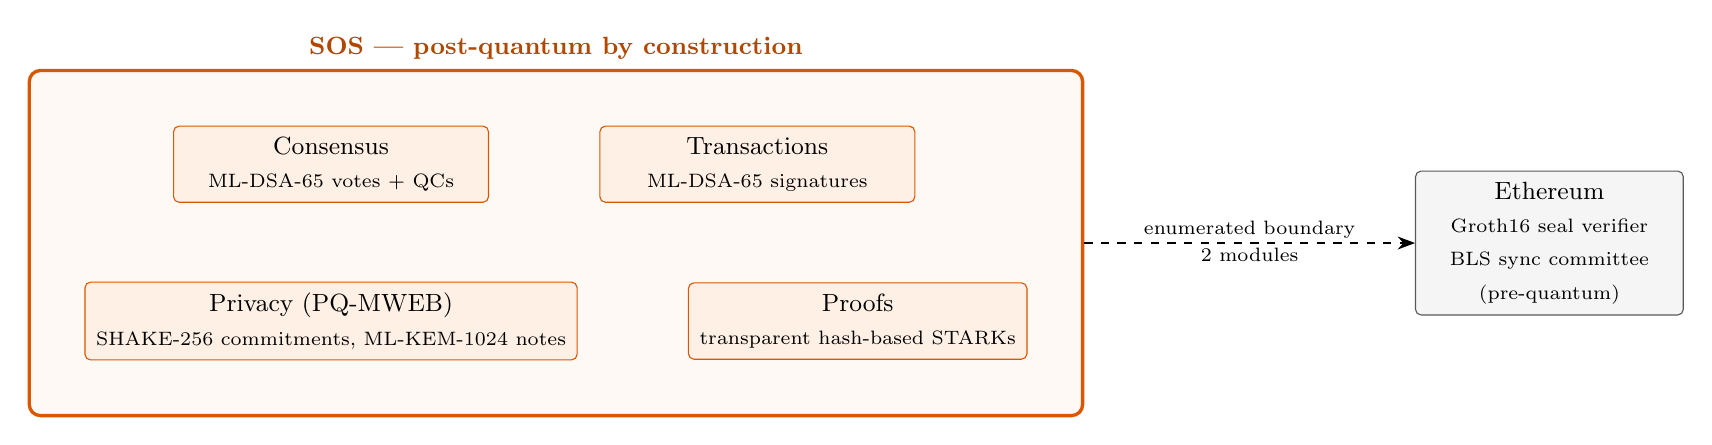
\begin{tikzpicture}[node distance=10mm and 14mm]
  \node[pqbox, minimum width=40mm] (a) {Consensus\\[1pt]{\scriptsize \mldsa{} votes + QCs}};
  \node[pqbox, minimum width=40mm, right=of a] (b) {Transactions\\[1pt]{\scriptsize \mldsa{} signatures}};
  \node[pqbox, minimum width=40mm, below=of a] (c) {Privacy (PQ-MWEB)\\[1pt]{\scriptsize \shake{} commitments, \mlkem{} notes}};
  \node[pqbox, minimum width=40mm, right=of c] (d) {Proofs\\[1pt]{\scriptsize transparent hash-based STARKs}};
  \begin{scope}[on background layer]
    \node[draw=sosorange!85!black, very thick, rounded corners, fill=sosorange!4,
          fit=(a)(b)(c)(d), inner sep=7mm,
          label={[font=\small\bfseries, text=sosorange!70!black]above:SOS --- post-quantum by construction}] (sosbox) {};
  \end{scope}
  \node[sbox, right=42mm of sosbox.east, anchor=west, minimum width=34mm] (eth)
        {Ethereum\\[1pt]{\scriptsize Groth16 seal verifier}\\[1pt]{\scriptsize BLS sync committee}\\[1pt]{\scriptsize (pre-quantum)}};
  \draw[darr] (sosbox.east) -- node[el, above]{enumerated boundary} node[el, below]{2 modules} (eth.west);
\end{tikzpicture}}%
\caption{The post-quantum discipline. All primitives inside the SOS perimeter
are post-quantum; pre-quantum cryptography appears only in the two
external-chain compatibility modules at the Ethereum boundary, and a quantum
break of either affects assets \emph{on Ethereum}, never the SOS ledger
(Section~\ref{sec:security}).}
\label{fig:boundary}
\end{figure}

\subsection{Contributions}
\label{sec:contributions}

This paper makes the following contributions. Each is developed in a dedicated
section with definitions, exact constructions, and security arguments; the
status tags are defined in Section~\ref{sec:status}.

\begin{enumerate}[leftmargin=1.6em]
\item \textbf{A coherent, fully post-quantum L1 protocol stack} \statusV{}
  (Sections~\ref{sec:prelim}--\ref{sec:consensus}): \mldsa{} for every
  signature including consensus votes; \shake{}/\sha{} for every hash,
  commitment, nullifier, and Merkle node with a global domain-separation
  registry (Appendix~\ref{app:domains}); \mlkem{} plus a \shake{}-KDF AEAD for
  note encryption; and bare hash-based STARKs for all succinct proofs the SOS
  network verifies.
\item \textbf{A zkVM-verifiable two-phase BFT proof-of-stake consensus}
  \statusV{} (Section~\ref{sec:consensus}): Tendermint-lineage two-phase
  locking (\code{lockedValue}/\code{lockedRound}, polka-gated unlock), strictly
  stake-weighted $>\!2/3$ quorum certificates of raw \mldsa{} signatures over a
  fixed 58-byte vote preimage, $f{+}1$ round synchronization, QC-gated
  catch-up, and a v4 block-hash preimage that binds \code{chain\_id},
  \code{epoch}, and the validator-set hash into the very hash the quorum
  signs --- the property the bridge and light clients rely on.
\item \textbf{PQ-MWEB} \statusI{} (Section~\ref{sec:privacy}): an opt-in
  shielded extension-block ledger re-derived from MWEB's deployment model
  \cite{mweb2020} and Zerocash-style accounting \cite{zerocash2014} with
  \emph{no} elliptic-curve algebra: hash-only ownership-welded commitments
  (\code{commit\_v3} binding $\mathit{npk} = H(\mathit{nk} \concat
  \mathit{ak})$), position-bound nullifiers, a depth-32 \shake{} commitment
  tree with a 256-root anchor window, \mlkem{}-sealed notes with one-byte view
  tags, per-action client-side STARKs with journal-as-truth verification, and
  binding of the entire pool state into the consensus application state root.
\item \textbf{A proof-based, non-custodial bidirectional SOS--Ethereum bridge}
  (Section~\ref{sec:bridge}): for SOS$\to$Ethereum, an in-zkVM verification of a real
  FIPS-204 stake-weighted quorum certificate ($\approx$5.87M zkVM cycles per
  signature, measured), composed with Merkle transaction-inclusion proofs in a
  batch guest whose committed journal is the exact ABI encoding that the
  on-chain \code{SOSBridge} contract reconstructs and verifies against a
  pinned, immutable program identity; for Ethereum$\to$SOS, a finality and
  execution-storage proof that extracts the wSOS burn under verified
  sync-committee roots. Both directions, the unattended relayer,
  and a public validator-set rotation from $V_0$ to $V_1$ have been demonstrated
  end-to-end against live Ethereum Sepolia with real proofs \statusI{};
  sustained cross-chain load/chaos exercise and external review remain
  \statusP{}.
\item \textbf{Proof-Carrying Finality and a measured acceleration program}
  (Section~\ref{sec:scalability}): a quantified analysis of the post-quantum
  quorum-certificate size problem, with negative results (committee sampling
  diverges as the Byzantine fraction approaches $1/3$; algebraic batch
  verification of distinct-signer ML-DSA is structurally unavailable; current
  lattice multi-signatures are not adoptable), a bounded-validator launch
  posture, an epoch-checkpoint finality certificate reusing the consensus
  STARK \statusI{}, measured zkVM acceleration levers (keccak accelerator,
  key-decode caching, multi-GPU shard composition) \statusM{}, and a native
  ML-DSA verification AIR prototype whose two feasibility kill-criteria both
  passed with measured data \statusM{}.
\item \textbf{A native, bit-exact FIPS-204 verification AIR with a measured
  in-zkVM re-verification crossover} \statusM{} (Section~\ref{sec:airtrack}):
  to our knowledge the first AIR family that arithmetizes measured cores of
  \emph{unmodified} FIPS-204 verification --- a fully range-checked mod-$q$
  multiplication gadget and the complete 8-layer forward NTT, bit-exact
  against the reference implementation --- in a transparent, hash-based FRI
  STARK, together with a \emph{wrap-not-replace} integration in which a thin
  zkVM guest verifies the native proof in software and journal-commits the
  result, leaving the recursion pipeline and the on-chain verifier untouched.
  Both pre-registered feasibility kill-criteria were retired with
  measurements: one NTT proves at $\approx 2\%$ of a full in-zkVM \mldsa{}
  verification budget, and the in-guest verification of the native proof
  costs $174.1$M cycles ($K^\ast \approx 47$), clearing the realistic
  67--128-signature quorum size. This is a measured research prototype with
  an explicit remaining program, not a deployed consensus primitive.
\item \textbf{An explicit threat model and TCB inventory}
  (Section~\ref{sec:security}): security claims with reductions to the stated
  assumptions, an enumeration of every trust boundary including the proof
  system's circuit TCB, and a list of known
  limitations stated against the actual code rather than the intended design.
\end{enumerate}

\subsection{Implementation status and honesty conventions}
\label{sec:status}

A whitepaper for an unlaunched system has an obligation not to blur design
intent with deployed fact. Throughout this paper every load-bearing component
carries one of four tags:

\begin{itemize}[leftmargin=1.6em]
\item \statusV{} --- implemented in the codebase \emph{and} exercised on a
  multi-node testnet under load and adversarial (chaos) conditions.
\item \statusI{} --- implemented in the codebase with passing unit and
  integration tests, not yet exercised by the full multi-node harness.
\item \statusP{} --- partially implemented; the remaining work is plumbing or
  integration, not open cryptography. The text states exactly what exists and
  what is missing.
\item \statusR{} / \statusM{} --- a research track; \statusM{} indicates the
  prototype exists and the numbers quoted are measurements, not estimates.
\end{itemize}

Three global caveats apply. First, the system is pre-mainnet and has not had an
external security audit; an internal adversarial audit program exists and its
findings (several of which materially changed the design, e.g.\ the
ownership-welding of Section~\ref{sec:ownership}) are folded into this paper.
Second, all performance figures are from the stated lab hardware and are
reproducible measurements, but they are not mainnet-scale benchmarks. Third,
where the live deployment or operating model lags the implemented cryptography
(notably independent operators and mainnet bridge migration,
Section~\ref{sec:bridge-status}), the paper says so explicitly.

\subsection{Organization}

Section~\ref{sec:prelim} fixes notation, defines the primitives, and states the
assumptions. Section~\ref{sec:overview} gives the system architecture.
Section~\ref{sec:consensus} specifies consensus and proves its safety.
Section~\ref{sec:economics} specifies monetary policy, the genesis distribution, and
staking. Section~\ref{sec:privacy} specifies PQ-MWEB.
Section~\ref{sec:bridge} specifies the Ethereum bridge in both directions.
Section~\ref{sec:scalability} presents the scalability analysis, PCF, and the
measured acceleration stack. Section~\ref{sec:airtrack} develops the native
FIPS-204 verification AIR --- architecture, gadget-level soundness arguments,
the in-guest verifier, and the measured crossover --- as a dedicated
contribution. Section~\ref{sec:security} gives the threat model and
security analysis. Section~\ref{sec:related} surveys related work.
Appendices~\ref{app:layouts}--\ref{app:params} collect the canonical byte
layouts with RFC-style wire-format diagrams, the domain-tag registry, and the
parameter tables.

% ============================================================================
\section{Preliminaries, Primitives, and Assumptions}
\label{sec:prelim}
% ============================================================================

\subsection{Notation}
\label{sec:notation}

All byte strings are finite sequences over $\{0,1\}^8$; $\concat$ denotes
concatenation. $\LE{k}(x)$ denotes the $k$-byte little-endian encoding of the
unsigned integer $x$; the implementation uses little-endian encodings in all
SOS-native preimages and big-endian 32-byte words only inside the
Ethereum-ABI journal (Section~\ref{sec:journal}), matching Solidity's
\code{abi.encode}.

For a fixed ASCII \emph{domain tag} $D$ we write
\[
H_D(m) \;=\; \mathrm{SHA3\text{-}256}(D \concat m),
\qquad
S_D(m_1,\dots,m_k) \;=\; \mathrm{SHAKE256}_{32}(D \concat m_1 \concat \cdots \concat m_k),
\]
where $\mathrm{SHAKE256}_{\ell}$ denotes $\ell$ bytes of \shake{} output. Domain
tags are versioned constants (e.g.\ \code{sos:note-commit:v3},
\code{bqp:block:v4}); the registry in Appendix~\ref{app:domains} lists every
tag in the protocol, and the implementation rule is that a tag is never reused
across purposes and never changed without a version bump and an activation
height. Two tag namespaces coexist for historical reasons: \code{bqp:} (the
project's original codename) and \code{sos:}; both are consensus-frozen
byte constants and the namespace carries no semantic distinction.

Validator voting power is denominated in \emph{stake} (Section~\ref{sec:staking});
a \emph{quorum} is any validator set whose summed effective stake is
\emph{strictly greater} than $2/3$ of the total active effective stake. Amounts
are integers in \emph{sats}, $10^{-8}$ SOS.

\subsection{ML-DSA-65 (FIPS 204)}
\label{sec:mldsa}

\mldsa{} is the module-lattice digital signature standard \cite{fips204}
derived from CRYSTALS-Dilithium \cite{dilithium2018}, instantiated at NIST
security category 3. Its EUF-CMA security reduces to the Module-LWE and
Module-SIS problems over power-of-two cyclotomic rings; no polynomial-time
quantum algorithm is known for either, and the parameter set targets a
classical/quantum security level comparable to AES-192. The concrete sizes
that shape the SOS protocol are:

\begin{center}
\begin{tabular}{@{}lrr@{}}
\toprule
 & \textbf{bytes} & \textbf{role in SOS} \\
\midrule
public key            & 1952 & validator \code{consensus\_pk}; account keys \\
signature             & 3309 & votes, QCs, transactions, spend authorization \\
\bottomrule
\end{tabular}
\end{center}

SOS uses \mldsa{} in its pure (non-pre-hash) mode with the \emph{empty
context string}: the signed message is the raw preimage defined by the
protocol (e.g.\ the 58-byte vote preimage of Construction~\ref{con:vote}).
This choice is consensus-critical --- the zkVM consensus guest
(Section~\ref{sec:consensus-guest}) re-verifies the same bytes with the same
FIPS-204 \code{Verify} algorithm, and any host/guest divergence in message
formatting is a soundness break, so a single shared library defines every
preimage on both sides. One \mldsa{} verification costs approximately $5.87$
million RISC-V cycles inside the zkVM used (measured;
Section~\ref{sec:accel}).

\begin{assumption}[ML-DSA unforgeability]
\label{ass:mldsa}
\mldsa{} is existentially unforgeable under adaptive chosen-message attack
(EUF-CMA) against quantum polynomial-time adversaries, per the Module-LWE and
Module-SIS assumptions at FIPS-204 category-3 parameters.
\end{assumption}

\subsection{ML-KEM-1024 (FIPS 203)}
\label{sec:mlkem}

\mlkem{} is the module-lattice key-encapsulation standard \cite{fips203}
derived from CRYSTALS-Kyber \cite{kyber2018}, instantiated at category 5
(the most conservative parameter set; ciphertext 1568 bytes, encapsulation
key 1568 bytes, 32-byte shared secret). SOS uses it solely for
\emph{note encryption} in the shielded pool: each note is sealed under a fresh
encapsulation against the recipient's registered KEM key
(Section~\ref{sec:notes-enc}), so note confidentiality is protected against a
harvest-now-decrypt-later adversary for the lifetime of the Module-LWE
assumption rather than the lifetime of an elliptic curve.

\begin{assumption}[ML-KEM CCA security]
\label{ass:mlkem}
\mlkem{} is IND-CCA2 secure against quantum polynomial-time adversaries at
FIPS-203 category-5 parameters.
\end{assumption}

\subsection{SHA-3, SHAKE-256, and the hash margin}
\label{sec:sha3}

\sha{} and \shake{} are the FIPS-202 \cite{fips202} sponge constructions over
Keccak-$f[1600]$. SOS uses \sha{} (fixed 32-byte output) for block hashes,
transaction hashes, validator identities, and the bridge journal digest's
inner components, and \shake{} (XOF, squeezed to 32 bytes unless stated) for
the entire note scheme and key-derivation paths. Against a quantum adversary,
Grover's algorithm bounds preimage search at $\Theta(2^{128})$ work for
32-byte outputs and the BHT algorithm bounds collisions at $\Theta(2^{85})$
query complexity (with classical collision search at $2^{128}$); both are
regarded as out of reach, and the sponge's indifferentiability supports the
domain-separation methodology of Section~\ref{sec:notation}.

\begin{assumption}[Hash security]
\label{ass:hash}
\sha{} and \shake{} (32-byte outputs) are collision-resistant, preimage-
resistant, and second-preimage-resistant against quantum polynomial-time
adversaries, and may be modelled as random oracles for the domain-separated
uses in this paper.
\end{assumption}

\subsection{ChaCha20-Poly1305}
\label{sec:aead}

Note plaintexts are encrypted under ChaCha20-Poly1305 \cite{rfc8439} with a key
and nonce derived by \shake{} from the \mlkem{} shared secret
(Section~\ref{sec:notes-enc}). Symmetric AEAD security degrades only by
Grover's quadratic factor (effective $\ge 2^{128}$ for the 256-bit key);
ChaCha20 is chosen over AES-GCM for constant-time software performance in
\code{no\_std} and WASM wallet environments, with no reliance on hardware AES.

\subsection{Hash-based commitments and nullifiers}
\label{sec:commitments}

\begin{definition}[Domain-separated hash commitment]
\label{def:commit}
For domain tag $D$, message tuple $m = (m_1,\dots,m_k)$ of fixed widths, and
trapdoor $r \in \{0,1\}^{256}$, the commitment is
$\mathrm{Com}_D(m; r) = S_D(m_1,\dots,m_k,r)$.
\emph{Binding} holds unconditionally up to collisions of \shake{}
(Assumption~\ref{ass:hash}): opening a commitment to two distinct tuples
exhibits a collision. \emph{Hiding} holds computationally in the random-oracle
model when $r$ has 256 bits of min-entropy: the adversary must query the
oracle on the correct $r$ to distinguish openings.
\end{definition}

This is deliberately the weakest, most conservative commitment in the design
space. Compared with algebraic (Pedersen-style) commitments it sacrifices
additive homomorphism --- so balance checks must be performed \emph{inside}
a zero-knowledge proof by explicit checked arithmetic
(Section~\ref{sec:circuits}) --- and gains two properties SOS considers
decisive: post-quantum security, and the absence of any algebraic structure
that an under-constrained circuit could exploit to counterfeit value, the bug
class that has repeatedly affected algebraic shielded-pool designs.

\begin{definition}[Nullifier]
\label{def:nullifier}
A nullifier scheme for a note commitment $cm$ is a deterministic function
$\mathit{nf} = \mathrm{NF}(\mathit{nk}, \rho, \mathit{pos})$ of a secret
nullifier key $\mathit{nk}$, a per-note value $\rho$ committed inside $cm$,
and the note's leaf position $\mathit{pos}$, such that (i) computing
$\mathit{nf}$ without $\mathit{nk}$ is infeasible; (ii) $\mathit{nf}$ reveals
nothing about which commitment it nullifies; and (iii) distinct notes yield
distinct nullifiers except with negligible probability. SOS instantiates
$\mathrm{NF} = S_{\code{sos:nullifier:v2}}(\mathit{nk}, \rho, \LE{8}(\mathit{pos}))$.
\end{definition}

\subsection{Transparent STARKs, FRI, and the RISC Zero zkVM}
\label{sec:starks}

A STARK \cite{starks2018} is a succinct, transparent argument of computational
integrity compiled from an interactive oracle proof \cite{bcs2016} whose
low-degree testing uses FRI \cite{fri2018} and whose only cryptographic
ingredient is a collision-resistant hash (for Merkle commitments and the
Fiat--Shamir transform). Transparency means there is no trusted setup and no
structured reference string; soundness rests on Assumption~\ref{ass:hash} plus
the proximity soundness of FRI. In the quantum random-oracle model,
hash-based IOP compilations of this family admit security proofs
\cite{cms2019}; accordingly STARKs are regarded as plausibly post-quantum, in
contrast to pairing-based SNARKs. We state the working assumption explicitly:

\begin{assumption}[Proof-system soundness]
\label{ass:stark}
The STARK system used (the RISC Zero zkVM \cite{risc0} proof system, and for
Section~\ref{sec:airtrack} the Plonky3 \cite{plonky3} uni-STARK --- over
Goldilocks in the measured prototype, over BabyBear in the production plan)
is computationally sound against quantum polynomial-time provers at its
documented conjectured soundness parameters: a prover cannot, except with
negligible probability, produce an accepting receipt for an execution that
does not correspond to running the committed program on some witness.
\end{assumption}

The RISC Zero zkVM proves correct execution of an arbitrary RISC-V
(rv32im) program, called a \emph{guest}. Three of its interfaces are
load-bearing for SOS:

\begin{itemize}[leftmargin=1.6em]
\item \textbf{Receipts and journals.} The prover emits a \emph{receipt}
  containing a seal (the STARK) and a \emph{journal} (the public outputs the
  guest committed via \code{env::commit}). A verifier checks the receipt
  against an \emph{image id} --- a 32-byte digest of the guest program binary
  --- and then trusts the journal as the program's authentic output. The image
  id is therefore part of consensus: SOS pins every guest's image id as a
  compile-time constant, with CI tests that fail on any drift
  (Sections~\ref{sec:batch-guest} and~\ref{sec:tcb}).
\item \textbf{Recursive composition.} A guest may call
  \code{env::verify(image\_id, journal)} to assert that a valid receipt exists
  for another program with exactly that journal; the host supplies the inner
  receipt as an \emph{assumption} and the recursion circuit discharges it.
  This is how the bridge folds a consensus proof and $n$ inclusion proofs into
  one receipt (Section~\ref{sec:batch-guest}).
\item \textbf{Receipt kinds.} The same proof can be emitted as a bare
  hash-based STARK receipt (composite or succinct) or wrapped into a Groth16
  proof over BN254 for cheap on-chain verification. SOS's discipline maps onto
  this directly: every SOS-internal verifier consumes the bare STARK; only
  the Ethereum-facing relayer produces the Groth16 wrap, and only the
  Ethereum contract verifies it (Sections~\ref{sec:nonpq}, \ref{sec:tcb}).
\end{itemize}

\subsection{Consensus and network assumptions}

\begin{assumption}[Byzantine stake bound]
\label{ass:byz}
At every height, validators controlling strictly less than $1/3$ of the total
active effective stake are Byzantine (arbitrarily malicious, including
quantum-capable); the remainder follow the protocol.
\end{assumption}

\begin{assumption}[Partial synchrony]
\label{ass:synchrony}
The network is partially synchronous in the sense of Dwork--Lynch--Stockmeyer
\cite{dls1988}: after an unknown global stabilization time, message delays
between honest nodes are bounded by an unknown constant. Safety must hold
without any timing assumption; liveness may rely on eventual synchrony.
\end{assumption}

\subsection{The post-quantum boundary, precisely}
\label{sec:boundary-def}

\begin{definition}[SOS-internal vs.\ external-chain compatibility]
\label{def:boundary}
A primitive use is \emph{SOS-internal} if its failure would allow forging SOS
state: a signature accepted by SOS consensus, a proof accepted by an SOS node,
a commitment or nullifier interpreted by the SOS ledger, or an encryption
protecting SOS secrets. A primitive use is an \emph{external-chain
compatibility module} if it is verified by, or verifies statements signed by,
a foreign chain, and its failure affects only assets or state on that foreign
chain. The SOS design rule is: every SOS-internal use is drawn from
$\{\mldsa{}, \mlkem{}, \sha{}/\shake{}, \text{ChaCha20-Poly1305},
\text{hash-based STARK}\}$; external-chain compatibility modules are
enumerated, currently exactly the Groth16/BN254 bridge seal
(Section~\ref{sec:nonpq}) and the BLS12-381 verification of the
Ethereum$\to$SOS light client (Section~\ref{sec:eth-to-sos}).
\end{definition}

% ============================================================================
\section{System Overview}
\label{sec:overview}
% ============================================================================

\subsection{Node architecture}

SOS is implemented in Rust as a single node binary exposing a JSON-RPC
interface to wallets, explorers, and tooling. One binary serves every role;
roles are configuration, not separate software (the ``model C'' decision:
every node validates; proving and relaying are opt-in modules, and a GPU is
never required to validate). The node's event loop drives four cooperating
subsystems:

\begin{itemize}[leftmargin=1.6em]
\item the \textbf{consensus reactor}: the two-phase BFT state machine of
  Section~\ref{sec:consensus} --- proposal handling, vote tallies, locking,
  round synchronization, QC construction and verification, and the catch-up
  buffer;
\item the \textbf{chain state machine}: applies finalized blocks; maintains
  the transparent UTXO set, the shielded pool (commitment tree, nullifier
  set, anchor window), the validator and staking state, and the supply
  tracker; computes the chained application state root \code{app\_hash}
  (Section~\ref{sec:apphash});
\item the \textbf{extension-block builder}: constructs and applies the
  private actions (shield, unshield, private transfer) of
  Section~\ref{sec:privacy}, enforcing journal-as-truth verification;
\item the \textbf{mempool}: admission, fee policy, and content-key
  deduplication (a canonical key over the action type, sender, amount, and
  burn identifier prevents duplicate logical actions from racing into blocks).
\end{itemize}

\begin{figure}[ht]\centering
\adjustbox{max width=\textwidth}{%
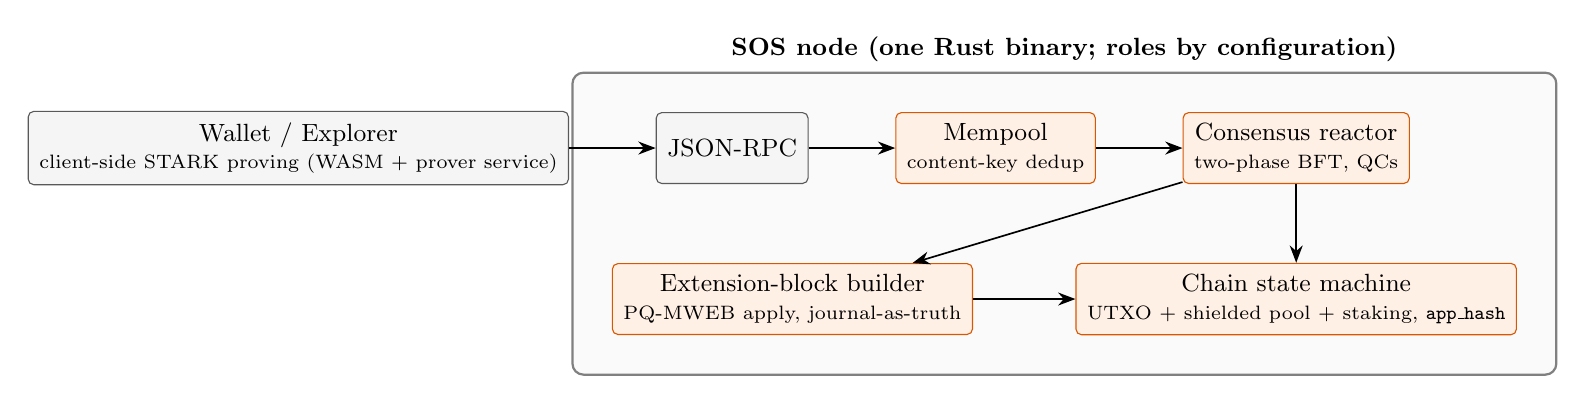
\begin{tikzpicture}[node distance=7mm and 11mm]
  \node[sbox, align=center] (wallet) {Wallet / Explorer\\[-1pt]{\scriptsize client-side STARK proving (WASM + prover service)}};
  \node[sbox, right=11mm of wallet] (rpc) {JSON-RPC};
  \node[pqbox, right=11mm of rpc] (mem) {Mempool\\[-1pt]{\scriptsize content-key dedup}};
  \node[pqbox, right=11mm of mem] (con) {Consensus reactor\\[-1pt]{\scriptsize two-phase BFT, QCs}};
  \node[pqbox, below=10mm of con] (chain) {Chain state machine\\[-1pt]{\scriptsize UTXO + shielded pool + staking, \code{app\_hash}}};
  \node[pqbox, left=13mm of chain] (ext) {Extension-block builder\\[-1pt]{\scriptsize PQ-MWEB apply, journal-as-truth}};
  \draw[arr] (wallet) -- (rpc);
  \draw[arr] (rpc) -- (mem);
  \draw[arr] (mem) -- (con);
  \draw[arr] (con) -- (chain);
  \draw[arr] (con) -- (ext);
  \draw[arr] (ext) -- (chain);
  \begin{scope}[on background layer]
    \node[draw=black!50, thick, rounded corners, fill=black!2,
          fit=(mem)(con)(ext)(chain), inner sep=5mm,
          label={[font=\small\bfseries]above:SOS node (one Rust binary; roles by configuration)}] {};
  \end{scope}
\end{tikzpicture}}%
\caption{Node architecture. Wallets prove privacy statements client-side and
the node only verifies; consensus finalizes blocks via two-phase BFT and the
chain state machine folds every state change --- transparent, shielded, and
staking --- into the chained \code{app\_hash} that validators vote on.}
\label{fig:arch}
\end{figure}

\subsection{Participants and roles}
\label{sec:roles}

\begin{itemize}[leftmargin=1.6em]
\item \textbf{Validators} hold bonded stake and an \mldsa{} consensus key,
  run the full state machine, and vote. Validation is CPU-only by design.
\item \textbf{Full/RPC nodes} follow consensus (verifying every block's QC),
  maintain full state, and serve wallets; they do not vote.
\item \textbf{Light clients} verify finality without state: given a block
  header and its embedded QC, a light client checks the stake-weighted
  \mldsa{} quorum against the known validator set
  (\code{verify\_qc}), with no ledger replay. Mobile wallets are light
  clients; a phone is never a validator (availability and slashing, not
  compute, are the binding constraints). The PCF certificate of
  Section~\ref{sec:pcf} is designed to replace per-block QC downloads with
  one constant-size STARK check per epoch.
\item \textbf{Privacy provers} are the users themselves: every private action
  is proved client-side, because the spend witness contains the secret
  nullifier key $\mathit{nk}$ whose disclosure delegates spend authority
  (Section~\ref{sec:client-proving}). The wallet talks to the user's own
  GPU-equipped prover (a hardened TLS service is provided) or proves locally.
  A prover that receives $\mathit{nk}$ must be treated as part of the user's
  trust boundary. Private transfer (private$\to$private) submission is now
  implemented with an \mldsa{} spend authorization inside the privacy STARK:
  the signed digest binds the chain id, expiry height, anchor, nullifiers,
  output commitments, output-ciphertext hashes, and fee. This prevents a node
  or prover from substituting different public effects for an accepted
  transfer, but it does not make third-party spend proving witness-private:
  delegated proving by an untrusted service remains outside the security
  claim.
\item \textbf{Bridge provers and relayers} are opt-in, permissionless,
  fee-compensated roles: the prover produces the recursive bridge STARK, the
  relayer wraps and submits it to Ethereum. Neither is trusted: a bad proof
  is rejected by the contract; liveness of these roles is an availability
  assumption, never a safety one.
\end{itemize}

\subsection{Transaction classes and the state root}
\label{sec:apphash}

A transaction is \emph{transparent} by default --- a UTXO transfer authorized
by an \mldsa{} signature --- or \emph{private}, routed through the extension
block (shield, private transfer, unshield). Every finalized block commits to
the post-state via the chained \code{app\_hash}: a \sha{} digest over
canonical encodings of (i) the UTXO set root, (ii) the \emph{contents} of the
shielded pool --- note commitments, the commitment-tree root, the nullifier
set, and the rolling anchor window (domain \code{bqp:private-pool:v4}) ---
(iii) the supply tracker including the bridge-locked bucket,
and (iv) the validator and staking state including jailing flags. Two nodes
with equal \code{app\_hash} at equal height have byte-identical application
state. The block hash that validators sign binds \code{prev\_app\_hash}
(Section~\ref{sec:blockhash}), so a proposer that built on divergent state is
rejected at apply time, and --- after the audit finding discussed in
Section~\ref{sec:consensus-binding} --- \emph{every} shielded-pool change is
inside the quorum-signed perimeter.

\subsection{Zero-configuration networking and sync}
\label{sec:zeroconf}

A node ships with no required network configuration. On first start it
bootstraps from baked-in DNS seeds, discovers peers over the public internet,
and backfills the chain via a peer-to-peer block-sync protocol whose every
received block is admitted only through the same verified apply path as
live consensus (block-hash and QC verification, application against the prior
\code{app\_hash}), so a syncing node cannot be fed an invalid history. This has
been verified on the live public testnet: a fresh, unconfigured node joined
from the DNS seed, synced the chain from height zero, and its block hashes
matched the live chain bit-for-bit. The July 2026 fresh public testnet also
exposes its public P2P ingress on TCP~30303 through
\code{seed}, \code{seed1}, \code{seed2}, \code{seed3}, and
\code{dnsseed.soulofsatoshi.com}; all five records resolve to the same current
seed while the names remain independently rotatable. An external smoke test
that pinned the expected seed peer id (and therefore ignored unrelated mDNS
peers) completed the DNS-resolved libp2p handshake. DNS publication is an
operations property, not part of the consensus safety argument.
Local peer discovery (mDNS) and explicit \code{--boot-nodes} remain available
for private or lab deployments. \statusV{}

% ============================================================================
\section{Consensus}
\label{sec:consensus}
% ============================================================================

SOS finalizes blocks with a deterministic, two-phase, stake-weighted
Byzantine-fault-tolerant proof-of-stake protocol in the Tendermint lineage
\cite{tendermint2016,tendermint2018,pbft1999}. Three goals shaped it:
(a) classical BFT safety under Assumption~\ref{ass:byz} and liveness under
Assumption~\ref{ass:synchrony}; (b) post-quantum authentication of every
protocol message that bears on safety; and (c) --- unusual for a consensus
layer --- \emph{finality that is cheap and unambiguous to re-verify inside a
zkVM}, because the bridge (Section~\ref{sec:bridge}) and the PCF certificate
(Section~\ref{sec:pcf}) re-check it in a proof. Goal (c) drives concrete
choices that a conventional design would not make: fixed-width raw-byte vote
preimages instead of protobuf envelopes, a block hash that binds the validator
set itself, and quorum certificates embedded in blocks as first-class data.

This section is written to be implementable from the text alone; every byte
layout is the one in the code. \statusV{}

\subsection{Validators, stake, and the active set}
\label{sec:valset}

A validator is registered through a staking transaction carrying its 1952-byte
\mldsa{} \code{consensus\_pk}. Its identity is
$\mathit{id} = H_{\code{bqp:validator-pk:v1}}(\code{consensus\_pk})$, and its
voting power is its \emph{effective stake}
\[
\mathrm{stake}_{\mathrm{eff}}(v) \;=\; \mathrm{selfbond}(v) + \mathrm{delegated}(v),
\]
the sum of the operator's own bond and all delegations
(Section~\ref{sec:staking}). The \emph{active pool} at a height is the set of
registered validators that are neither jailed nor pending, ordered canonically
by (effective stake descending, id ascending); this canonical order is
consensus-critical because the validator-set hash
(Construction~\ref{con:valsethash}) is order-sensitive. Dynamic join is
supported: a new validator's bond enters a \emph{pending} state and activates
at a scheduled activation height, at which point membership flips
deterministically across all nodes within the same block (and is bound into
that block's \code{app\_hash}), so the active set and the quorum denominator
change simultaneously everywhere. Voluntary exit is implemented as a
consensus-key-authorized transaction. The removal height is derived as the
carrying block height plus ten blocks; until that boundary the validator
continues to vote and count in the denominator, then every node removes it
simultaneously and binds the change into \code{app\_hash}. Self-bond and
third-party delegations enter the 21-day unbonding queue of
Section~\ref{sec:staking}. An exit is rejected if it would leave fewer than
four active validators. The protocol supports a registered pool of up to
$200$ validators and bounds proposer eligibility to the top $64$ by effective
stake; these limits sit within the bounded-active-set posture of
Section~\ref{sec:bounded} ($N \le 128$ active consensus participants).

\subsection{The canonical block hash (v4)}
\label{sec:blockhash}

\begin{construction}[Block hash \code{bqp:block:v4}]
\label{con:blockhash}
For a block at height $h$ in slot $s$, with transparent transaction root
\code{tx\_root}, post-state UTXO root \code{utxo\_root}, extension-block root
\code{ext\_root}, parent application state root \code{prev\_app\_hash}, chain
identity \code{chain\_id} (a 4-byte constant; the current network uses
\code{0x534F53}), epoch number $e$, and validator-set hash $V$
(Construction~\ref{con:valsethash}):
\[
\begin{aligned}
\code{block\_hash} = H_{\code{bqp:block:v4}}\big(
  &\LE{4}(\code{chain\_id}) \concat \LE{4}(e) \concat V \concat \LE{8}(h) \concat \LE{8}(s) \\
  &\concat \code{tx\_root} \concat \code{utxo\_root} \concat \code{ext\_root} \concat \code{prev\_app\_hash}\big).
\end{aligned}
\]
The preimage is fixed-width (184 bytes after the tag) with no separators;
Appendix~\ref{app:layouts} tabulates the offsets and
Figure~\ref{fig:wire-blockhash} renders the layout. Earlier preimage versions
(v2: $h, s, \code{tx\_root}, \code{utxo\_root}$; v3: v2 plus
\code{ext\_root}, \code{prev\_app\_hash}) remain defined behind a
protocol-version gate for historical blocks.
\end{construction}

\begin{construction}[Validator-set hash]
\label{con:valsethash}
For the active pool $(v_1, \dots, v_n)$ in canonical order,
\[
\begin{aligned}
V = H_{\code{sos:bridge-valset:v2}}\big(
  &\code{consensus\_pk}(v_1) \concat \LE{8}(\mathrm{stake}_{\mathrm{eff}}(v_1)) \concat \cdots \\
  &\concat \code{consensus\_pk}(v_n) \concat \LE{8}(\mathrm{stake}_{\mathrm{eff}}(v_n))\big),
\end{aligned}
\]
i.e.\ a \sha{} digest over each validator's full 1952-byte key and 8-byte
little-endian effective stake, in active-pool order. $V$ is order- and
stake-sensitive by construction (a reordered set or a restaked validator
yields a different $V$; this is pinned by tests). The hash input is rendered
in Figure~\ref{fig:wire-valset}.
\end{construction}

The v4 binding deserves emphasis because it is the hinge of the bridge's
security argument. Because the quorum certificate consists of signatures over
\code{block\_hash}, folding \code{chain\_id}, $e$, and $V$ into the hash makes
the quorum \emph{cryptographically attest} three statements that a verifier
holding only the QC (a light client, or the zkVM guest) could otherwise not
establish: that the block belongs to this chain and not a testnet or fork
(anti-replay across chains); that it belongs to the claimed epoch (anti-replay
across validator-set generations); and \emph{which validator set is canonical
at this height} --- so a prover cannot present a quorum of signatures checked
against a substitute validator set of its own choosing
(Section~\ref{sec:bridge-soundness}). Binding \code{prev\_app\_hash} chains
the application state: a proposer that built on divergent state produces a
hash no honest validator will sign, and a syncing node rejects a block whose
claimed parent root disagrees with its own.

\subsection{Votes and the 58-byte preimage}
\label{sec:votes}

\begin{construction}[Vote preimage]
\label{con:vote}
A consensus vote is an \mldsa{} signature (empty context, raw message) over
the 58-byte preimage
\[
\code{"SOSVOTE2"} \;(8) \concat \LE{4}(\code{chain\_id}) \concat \code{block\_hash} \;(32) \concat
\LE{8}(h) \concat \LE{4}(r) \concat \mathit{phase} \;(1) \concat
\mathit{nil} \;(1),
\]
where $r$ is the round, $\mathit{phase} = 0$ for \textsc{prevote} and $1$ for
\textsc{precommit}, and $\mathit{nil} = 1$ iff $\code{block\_hash}$ is the
all-zero hash (a nil vote), else $0$.
\end{construction}

Every field exists to kill a replay class, and each was motivated by a
concrete defect found in an earlier iteration of the live path: the domain
tag separates vote signatures from block-proposer signatures made with the
same key (previously a proposer's block signature was byte-identical to a
vote); the chain-id field makes even nil votes non-replayable across forks
or testnets; the height and round bind the vote to its position (previously a nil
vote signed the same 32 zero bytes at every height --- free equivocation
material); the phase byte makes a \textsc{prevote} signature unusable as a
\textsc{precommit}, so a quorum certificate (which is a precommit-domain
object) cannot be assembled from prevotes; and the nil byte separates
``no value'' from a vote for a value. A single shared function constructs
this preimage at every signing site, at the node's verification site, and in
the zkVM guests; its layout is pinned by byte-offset tests on both sides and
rendered in Figure~\ref{fig:wire-vote}.

\subsection{The two-phase protocol}
\label{sec:twophase}

Each height $h$ proceeds in rounds $r = 0, 1, 2, \dots$; each round has three
steps: \textsc{propose}, \textsc{prevote}, \textsc{precommit}. The round-$r$
proposer is selected deterministically and proportionally to effective stake
from the eligible active set by the construction of
Section~\ref{sec:proposer}, so all honest nodes agree on it without
communication. Each node
maintains the Tendermint lock state: $\mathit{lockedValue} \in
\{\bot\} \cup \{0,1\}^{256}$ and $\mathit{lockedRound} \in \{-1, 0, 1, \dots\}$,
plus $\mathit{validValue}/\mathit{validRound}$, all reset only at a new
height (a new height starts unlocked; a new \emph{round} preserves locks and
all vote tallies).

\begin{description}[leftmargin=1.6em, style=nextline]
\item[\textsc{propose}.] The round's proposer broadcasts a block (or
  re-proposes its locked value, attaching the round $vr$ at which that value
  last obtained a prevote quorum). Non-proposers wait for the proposal or a
  timeout.
\item[\textsc{prevote}.] On a proposal for value $v$ (hash $\hat{v} \ne 0$)
  with valid-round $vr$, a node prevotes $\hat{v}$ iff
  \[
  \mathit{lockedRound} = -1
  \;\lor\; \mathit{lockedValue} = \hat{v}
  \;\lor\; \big( vr \ge 0 \,\land\, vr \ge \mathit{lockedRound} \,\land\,
  \mathrm{polka}(vr) = \hat{v} \big),
  \]
  where $\mathrm{polka}(vr) = \hat{v}$ means the node has \emph{locally
  observed}, in its own tally, prevotes for $\hat{v}$ at round $vr$ from
  validators holding strictly more than $2/3$ of total stake. The polka check
  is local by design: no quorum certificate attached to a proposal is
  trusted on the wire; the proposer's $vr$ is only a pointer telling the node
  where in its own tallies to look. Note $vr \ge \mathit{lockedRound}$ (with
  equality unlocking) is required for liveness, and $vr < \mathit{lockedRound}$
  must not unlock for safety. Otherwise the node prevotes nil.
\item[\textsc{precommit}.] On observing a polka for $\hat{v}$ at the current
  round, the node sets $\mathit{lockedValue} \gets \hat{v}$,
  $\mathit{lockedRound} \gets r$, records $\hat{v}$ as its valid value, and
  precommits $\hat{v}$. Otherwise, on timeout, it precommits nil.
\item[\textsc{commit}.] A block commits at a node when the node observes
  precommits for one non-nil $\hat{v}$ at any single round from validators
  holding strictly more than $2/3$ of total stake. The committing node
  materializes the quorum certificate (Section~\ref{sec:qc}), applies the
  block, and advances to height $h+1$ unlocked.
\end{description}

All thresholds are \emph{stake-weighted with strict inequalities}: a set $S$
of distinct validators meets the $2/3$ threshold iff
$3 \sum_{v \in S} \mathrm{stake}_{\mathrm{eff}}(v) > 2 \cdot T$ where $T$ is
total active stake, and the $f{+}1$ threshold iff
$3 \sum_{v \in S} \mathrm{stake}_{\mathrm{eff}}(v) > T$. Duplicate voters
count once; per-round anti-equivocation tracking refuses to tally two
different-hash votes of the same type from one validator at one $(h, r)$ and
retains both signatures as slashing evidence
(Section~\ref{sec:slashing}). (For bootstrap configurations whose validators
have placeholder keys, the implementation falls back to head-count
thresholds; any set containing a real key uses stake weighting. This is a
development convenience, not a protocol mode.)

Phase timeouts escalate linearly with the round number
($\mathit{timeout}(r) = \mathit{base} + 1000\,\mathrm{ms} \cdot r$), the
standard partial-synchrony device for eventually exceeding the unknown
network delay.

Commit skew creates one additional delivery case: a node still applying height
$h$ can receive the proposal and votes for $h{+}1$, and gossipsub need not send
those messages a second time. The reactor therefore keeps a bounded,
\emph{liveness-only} one-height look-ahead buffer. A future proposal is not
acted on early; after entering $h{+}1$ it is removed and replayed through the
full proposal-validation path against the committed parent state and the
epoch-frozen active set. Future votes are retained only after their \mldsa{}
signatures verify, with a cap of $1024$ entries, and are replayed in
prevote-before-precommit order through the normal signature, equivocation,
quorum, and round-synchronization checks. No buffered message bypasses a safety
predicate, and messages more than one height ahead are dropped. \statusV{}

\begin{figure}[ht]\centering
\adjustbox{max width=\textwidth}{%
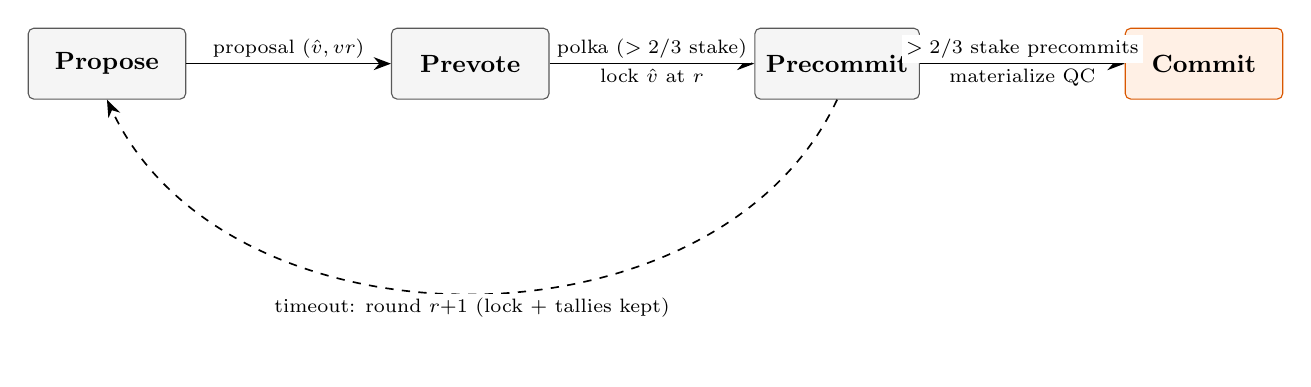
\begin{tikzpicture}[node distance=26mm]
  \node[sbox, minimum width=20mm, font=\small\bfseries] (prop) {Propose};
  \node[sbox, minimum width=20mm, font=\small\bfseries, right=of prop] (prev) {Prevote};
  \node[sbox, minimum width=20mm, font=\small\bfseries, right=of prev] (prec) {Precommit};
  \node[pqbox, minimum width=20mm, font=\small\bfseries, right=of prec] (com) {Commit};
  \draw[arr] (prop) -- node[el,above]{proposal $(\hat v, vr)$} (prev);
  \draw[arr] (prev) -- node[el,above]{polka ($>2/3$ stake)} node[el,below]{lock $\hat v$ at $r$} (prec);
  \draw[arr] (prec) -- node[el,above]{$>2/3$ stake precommits} node[el,below]{materialize QC} (com);
  \draw[darr] (prec.south) to[out=-115,in=-65] node[el,below]{timeout: round $r{+}1$ (lock + tallies kept)} (prop.south);
\end{tikzpicture}}%
\caption{One round of the two-phase protocol. Locks and vote tallies survive
round changes; only a polka at a round $\ge$ the locked round unlocks a node.
The $f{+}1$ round-synchronization rule (Section~\ref{sec:liveness}) keeps
honest nodes in the same round under timeout skew.}
\label{fig:consensus}
\end{figure}

\subsection{Quorum certificates}
\label{sec:qc}

\begin{construction}[Quorum certificate]
\label{con:qc}
When a block commits at round $r^\ast$, the committing proposer attaches to
the block a QC: the pair $(r^\ast, \{(\mathit{id}_i, \sigma_i)\}_i)$ where
each $\sigma_i$ is validator $i$'s raw 3309-byte \mldsa{} precommit signature
over the preimage of Construction~\ref{con:vote} with
$\mathit{phase} = 1$. Verification (\code{verify\_qc}) recomputes the
preimage from $(\code{block\_hash}, h, r^\ast)$, verifies each signature
against the registered \code{consensus\_pk}, sums the effective stake of
\emph{distinct, valid} signers, and accepts iff
$3\cdot\mathrm{signed} > 2\cdot T$. Verification is fail-closed: unknown
voters, duplicate voters, malformed fields, or a zero-stake set contribute
nothing or reject outright.
\end{construction}

The QC is deliberately \emph{not} folded into the block hash (the votes are
over the hash; including them would be circular), so attaching it never
perturbs \code{app\_hash}. Its role is to make finality \emph{portable}: a
node syncing from block data alone, a light client, and the zkVM consensus
guest all run the same check against the same bytes, with no trust in the
serving peer. The QC is also the protocol's main scalability liability ---
one full \mldsa{} signature per signer --- quantified and addressed in
Section~\ref{sec:scalability}.

\subsection{Safety}
\label{sec:safety}

\begin{lemma}[Quorum intersection]
\label{lem:intersect}
Under Assumption~\ref{ass:byz}, any two sets of validators each holding
strictly more than $2/3$ of total stake share at least one honest validator.
\end{lemma}

\begin{proof}
Let the sets hold stake $a$ and $b$ with $3a > 2T$ and $3b > 2T$. Their
union holds at most $T$, so their intersection holds at least
$a + b - T > \tfrac{2T}{3} + \tfrac{2T}{3} - T = \tfrac{T}{3}$. Since
Byzantine validators hold strictly less than $T/3$, the intersection's stake
strictly exceeds the total Byzantine stake, so it contains an honest
validator.
\end{proof}

\begin{theorem}[Safety]
\label{thm:safety}
Under Assumptions~\ref{ass:mldsa} and~\ref{ass:byz}, no two honest nodes
commit different blocks at the same height, regardless of timing.
\end{theorem}

\begin{proof}[Proof sketch]
Suppose honest nodes commit distinct values $v \ne v'$ at height $h$, at
rounds $r \le r'$. Each commit requires a precommit quorum
(Construction~\ref{con:qc}); by Assumption~\ref{ass:mldsa} every counted
precommit was produced by the keyed validator, so the quorums are real sets
of validators.

\emph{Case $r = r'$:} the two precommit quorums intersect in an honest
validator (Lemma~\ref{lem:intersect}) that precommitted both $v$ and $v'$ at
the same round, which the protocol forbids (one precommit per round,
enforced by per-round anti-equivocation; an honest node precommits only on a
polka for a single value, and at most one value can obtain a polka per round
because two polka quorums would themselves intersect in an honest prevoter
who prevoted twice).

\emph{Case $r < r'$:} consider the precommit quorum $Q$ for $v$ at $r$. Every
honest member of $Q$ (more than $T/3$ stake worth, by the argument of
Lemma~\ref{lem:intersect} applied against the Byzantine bound) set
$\mathit{lockedValue} = v$, $\mathit{lockedRound} = r$ upon precommitting.
Take the smallest round $r'' \in (r, r']$ at which any polka for a value
$w \ne v$ occurs. A polka at $r''$ requires prevotes from a $>\!2/3$-stake
quorum, which intersects $Q$ in an honest validator $u$
(Lemma~\ref{lem:intersect}). At round $r''$, $u$ is still locked on $v$ with
$\mathit{lockedRound} \ge r$ (locks persist across rounds and only move
forward), and the prevote rule allows $u$ to prevote $w \ne v$ only upon
locally observing a polka for $w$ at some $vr \ge \mathit{lockedRound}$ with
$vr < r''$ --- contradicting the minimality of $r''$. Hence no polka, no
precommit quorum, and no commit for any $w \ne v$ at any round in
$(r, r']$.
\end{proof}

The cross-round case is precisely the scenario that was reproduced as a fork
on an earlier, single-phase iteration of the implementation and is now closed
by the lock rule; the reproduction is retained as a regression test, and an
independent re-audit of the live code (June 2026) confirmed the two-phase
logic and that the guest-verified preimage matches the live 58-byte
precommit. \statusV{}

\subsection{Liveness under partial synchrony}
\label{sec:liveness}

A faithful two-phase protocol is safe unconditionally, but three further
mechanisms proved necessary on a real lossy network to obtain liveness; all
three were added in response to observed stalls in load/chaos testing, and
all three preserve the safety argument because none touches the lock rule.

\begin{itemize}[leftmargin=1.6em]
\item \textbf{$f{+}1$ round synchronization.} If a node observes votes
  (either phase) at a round $r^+$ greater than its own from validators
  holding strictly more than $1/3$ of total stake, then at least one
  \emph{honest} validator is at $r^+$ (Byzantine stake cannot reach $1/3$),
  so the node fast-forwards to $r^+$, preserving its lock and all tallies and
  re-entering \textsc{propose}. Without this rule, nodes whose timeouts fire
  at slightly different moments drift into different rounds and no proposal
  ever gathers a quorum --- a livelock observed empirically under load.
\item \textbf{QC-gated catch-up.} A node that falls behind buffers
  out-of-order blocks and applies a buffered block only if it carries a QC
  that verifies under Construction~\ref{con:qc}; a bare gossiped proposal is
  never applied. Two subtle wedges in this path were found and fixed by the
  chaos suite: a buffered QC-\emph{less} copy of a height must not suppress
  re-fetching a QC-bearing copy, and the buffer eviction policy must evict
  far-future heights rather than the next-needed one (the naive
  evict-lowest policy permanently wedged any node that fell more than the
  buffer size behind).
\item \textbf{Consensus-envelope block budgeting.} The proposer's transaction
  budget is the apply-time block-size ceiling (4\,MiB) \emph{minus} the
  consensus envelope it will add: the proposer key and signature and the QC,
  which carries one 3309-byte signature per potential signer. A builder that
  counts only transaction bytes emits a block that every node rejects at
  apply time and then re-proposes forever --- a deterministic halt observed
  in testing and eliminated by reserving the envelope.
\end{itemize}

\begin{proposition}[Liveness, informal]
Under Assumptions~\ref{ass:byz} and~\ref{ass:synchrony}, after the global
stabilization time every height terminates: timeout escalation eventually
exceeds the message delay; the without-replacement proposer cycle selects an
online proposer within at most $N$ rounds from round zero (and in fewer than
$2N$ rounds from an arbitrary point across a cycle boundary), and the $f{+}1$ rule brings all
honest validators into that common round;
and the prevote rule's $vr \ge \mathit{lockedRound}$ clause (with equality
unlocking) guarantees that a value locked by some honest node in an earlier
round can be re-proposed and adopted by all honest nodes, so no permanent
lock-split persists.
\end{proposition}

\subsection{Equivocation, slashing, and accountability}
\label{sec:slashing}

Because every vote is a position-bound \mldsa{} signature, misbehaviour is
self-evidencing: two verified precommits from the same validator at the same
$(h, r)$ with different block hashes constitute complete, transferable
evidence of double-signing, with no additional context needed. Evidence is
applied deterministically in a later block. As implemented today, the
slashable on-chain evidence path is consensus double-signing, with a
$500$\,bps ($5\%$) burn from the offender's effective stake; downtime is
enforced as jailing. Additional penalty constants for committee equivocation,
invalid bridge batches, and downtime burns are reserved in code but are not
yet wired as launch-grade evidence types. The mainnet release gate is to
either wire and test those evidence paths end-to-end or keep the public
economics limited to double-sign slashing plus downtime jail. \statusP{}

\subsection{Proposer selection}
\label{sec:proposer}

The round-$r$ proposer at height $h$ is selected deterministically from the
top 64 validators of the canonical active pool by a stake-weighted permutation
without replacement. Let $N$ be the eligible count, $c=\lfloor r/N\rfloor$,
and $j=r\bmod N$. For draw $k=0,\ldots,j$, the implementation hashes
\code{u64le(h) || u32le(c) || u32le(k)} under
\code{sos:weighted-proposer:v2}, reduces the first 128 digest bits modulo the
remaining effective stake, walks the canonical cumulative-weight intervals,
selects that validator, and removes it before the next draw. If all remaining
weights are zero, the same digest selects an index among them. The first draw
is therefore exactly stake-proportional and splitting one stake interval does
not increase its aggregate primary-proposer probability; without-replacement
fallback also guarantees that no validator occupies two slots in one cycle.
Consequently, if any eligible validator is online, an online proposer appears
within at most $N$ rounds from the start of a height. From an arbitrary point
inside a cycle the conservative bound is fewer than $2N$ rounds, because the
remaining online slots may already have passed and the next independently
permuted cycle may place them late. This closes the unbounded
repeated-offline-proposer streak observed under the v1 independent-round lottery. Selection remains
communication-free. \statusI{}

\subsection{Empirical validation}
\label{sec:consensus-eval}

The consensus and value path were exercised on a four-node local testnet
driven by a load/chaos harness, with a 200\,ms consensus tick. Headline
results (all \statusV{}): hundreds of concurrent transparent transfers commit
with zero supply drift and byte-identical \code{app\_hash} across nodes; a
double-spend race (the same funds raced to two recipients via two nodes)
settles exactly one output, never both; killing more than $1/3$ of stake
halts the chain without forking and restoring quorum resumes it; floods of
invalid and overspending transactions are rejected without a node panic; a
reproduced cross-round fork scenario is closed by the lock rule
(regression-tested); a $2$--$2$ sub-quorum vote split that livelocks a
single-phase design converges; and the happy path commits in approximately
$600$\,ms per block. On the July 2026 fresh public testnet, a three-validator
deployment finalizes with $3/3$ precommits and a measured interval still around
the sub-second range; because this is a small co-located deployment, it is not
directly comparable to the four-node chaos latency above. The validators first
completed a one-at-a-time rollout of a pure
\code{--no-default-features --features verify-only} binary. Activating the
consensus-visible proposer-v2 schedule then used a coordinated stop/install/start
on all three validators, without replacing or copying a data directory. The
nodes had stopped at height~35642 with a v1 vote already persisted for 35643;
the vote WAL refused a conflicting re-sign after restart, synchronized that
already-finalized block, and made height~35644 the first full proposer-v2
height. The active binary has SHA-256 \code{9f58f038\ldots 8789b}; all three
independently reported height~35732, block hash
\code{a04c61bb\ldots b2d2c0}, and application hash
\code{2529c923\ldots ead8a}. Expected and actual supply both remained
$210{,}000{,}000{,}000{,}000$ sats. Stopping node 0 caused the public HTTPS RPC
to serve the finalized chain through a backup validator in 321\,ms; node 0 then
restarted and all three reconverged at height~35823. Separately, a clean
deterministic proposer-v2 four-validator-plus-observer chaos run lasted
723.5\,s, made 720 invariant checks, injected 22
kill/restart/partition/delay/flood events, accepted 1,489 mixed
transfer/stake/undelegate operations, and ended at height~113 with no fork,
state divergence, supply drift, or liveness violation. The genesis
\code{slot\_time\_secs} of $5$ is a nominal parameter that
the current reactor does not enforce as a block interval: block production is
tick-driven at $200$\,ms and paced by quorum formation, while the
$\approx 5$\,s timeouts in the reactor are round/view-change timeouts that bound
a round before a view change, not the inter-block time. These are functional
and adversarial results on small networks, not throughput claims.

% ============================================================================
\section{Tokenomics: Monetary Policy, Distribution, and Staking}
\label{sec:economics}
% ============================================================================

This section gives the complete tokenomics of \sos{}. Every quantity is read
from the authoritative \code{genesis.json} for \code{genesis-v2}
($1\,\mathrm{SOS} = 10^8$ sats) and is reconciled to the supply invariant
(Invariant~\ref{inv:supply}): genesis $2{,}100{,}000$ SOS $=$ liquid
$210{,}000$ $+$ bonded $40{,}000$ $+$ vesting-locked $1{,}850{,}000$, and
genesis $+$ emission pool $= 21{,}000{,}000$ SOS. Genesis-frozen figures are
\statusV{}; monetary-policy mechanics are \statusI{}; the staking yields of
Section~\ref{sec:staking} are \emph{illustrative}, not measured, and are
labelled as such.

\subsection{Tokenomics at a glance}
\label{sec:tokenomics-summary}

\begin{table}[ht]\centering
\adjustbox{max width=\textwidth}{%
\small
\begin{tabular}{@{}ll@{}}
\toprule
\textbf{parameter} & \textbf{value} \\
\midrule
unit / smallest denomination & SOS; $1\,\mathrm{SOS} = 10^8$ sats \\
chain id                     & \code{0x534F53} \\
supply cap                   & $21{,}000{,}000$ SOS (hard, invariant-enforced) \\
genesis supply               & $2{,}100{,}000$ SOS ($10\%$ of cap) \\
emission pool                & $18{,}900{,}000$ SOS ($90\%$ of cap) \\
liquid at genesis            & $210{,}000$ SOS \\
bonded at genesis            & $40{,}000$ SOS (initial-validator self-bond) \\
vesting-locked at genesis    & $1{,}850{,}000$ SOS \\
emission rate                & $210{,}000$ SOS/yr flat; cap-truncated ($\approx$ year $90$) \\
epoch length                 & $7$ days ($52$ epochs/yr) \\
reward split                 & $70\%$ stakers / $20\%$ operators / $10\%$ treasury \\
fee policy                   & $30\%$ of each fee burned, $70\%$ distributed \\
unbonding period             & $21$ days \\
\bottomrule
\end{tabular}}
\caption{Tokenomics at a glance (\code{genesis-v2}). Genesis-frozen figures
\statusV{}; monetary-policy mechanics \statusI{}.}
\label{tab:tokenomics}
\end{table}

\subsection{Units and supply cap}

The unit of account is the SOS; amounts are integers in sats
($1\,\mathrm{SOS} = 10^8$ sats). The hard supply cap is
\[
\textsf{SUPPLY\_CAP} \;=\; 21{,}000{,}000 \;\mathrm{SOS}
\;=\; 2.1 \times 10^{15} \,\text{sats},
\]
deliberately echoing Bitcoin \cite{nakamoto2008}. The cap is not a social
convention: it is enforced every block by the supply invariant of
Section~\ref{sec:invariant}, whose violation halts the node.

\subsection{Genesis distribution}
\label{sec:claim}

The launch genesis (\code{genesis-v2}, chain id \code{0x534F53}) mints a fixed
\emph{genesis supply} of $2{,}100{,}000$ SOS --- exactly $10\%$ of the
$21{,}000{,}000$ cap --- and leaves the remaining $18{,}900{,}000$ SOS ($90\%$)
in an \emph{emission pool} issued over time by the bounded emission of
Section~\ref{sec:emission}. The genesis supply is partitioned into six
categories, each with an explicit on-chain vesting schedule in epochs of
$7$ days; every figure below is taken directly from the authoritative genesis
file and is reconciled against the supply invariant
(Invariant~\ref{inv:supply}) from block zero. \statusV{}

\begin{center}
\adjustbox{max width=\textwidth}{%
\small
\begin{tabular}{@{}lrrr@{}}
\toprule
\textbf{supply component} & \textbf{sats} & \textbf{SOS} & \textbf{\% of cap} \\
\midrule
supply cap                            & $2{,}100{,}000{,}000{,}000{,}000$ & $21{,}000{,}000$ & $100\%$ \\
\quad genesis supply (minted at block 0)  & $210{,}000{,}000{,}000{,}000$     & $2{,}100{,}000$  & $10\%$ \\
\quad emission pool (issued as rewards)   & $1{,}890{,}000{,}000{,}000{,}000$ & $18{,}900{,}000$ & $90\%$ \\
\midrule
\quad\quad liquid at genesis          & $21{,}000{,}000{,}000{,}000$      & $210{,}000$      & --- \\
\quad\quad bonded at genesis          & $4{,}000{,}000{,}000{,}000$       & $40{,}000$       & --- \\
\quad\quad vesting-locked at genesis  & $185{,}000{,}000{,}000{,}000$     & $1{,}850{,}000$  & --- \\
\bottomrule
\end{tabular}}
\end{center}

\begin{center}
\adjustbox{max width=\textwidth}{%
\small
\begin{tabular}{@{}lrrccr@{}}
\toprule
\textbf{category} & \textbf{total} & \textbf{liquid @ gen.} & \textbf{cliff} & \textbf{linear} & \textbf{on sched.} \\
                  & \textbf{(SOS)} & \textbf{(SOS)}         & \textbf{(ep.)} & \textbf{(ep.)}  & \textbf{(SOS)} \\
\midrule
team      & $840{,}000$        & $0$          & $52$ & $156$ & $820{,}000$ \\
treasury  & $420{,}000$        & $0$          & $0$  & $260$ & $400{,}000$ \\
community & $315{,}000$        & $0$          & $0$  & $156$ & $315{,}000$ \\
airdrop   & $210{,}000$        & $52{,}500$   & $0$  & $52$  & $157{,}500$ \\
marketing & $157{,}500$        & $0$          & $26$ & $104$ & $157{,}500$ \\
liquidity & $157{,}500$        & $157{,}500$  & ---  & ---   & $0$ \\
\midrule
\textbf{total} & $\mathbf{2{,}100{,}000}$ & $\mathbf{210{,}000}$ & & & \\
\bottomrule
\end{tabular}}
\end{center}

Vesting is linear per epoch after an optional cliff and is tracked on-chain, so
an account's spendable balance at epoch $t$ is its genesis-liquid amount plus
the matured fraction of its scheduled total. Two categories carry liquid supply
at block zero --- the liquidity allocation (fully liquid) and part of the
airdrop allocation --- totalling $210{,}000$ SOS; a further $40{,}000$ SOS is
bonded at genesis as the self-bond of the initial validators, and the remaining
$1{,}850{,}000$ SOS is vesting-locked.\footnote{For the team and treasury
categories the \code{total} exceeds the vesting-schedule total by $20{,}000$
SOS each; that $40{,}000$ SOS is the genesis validators' self-bond (each of the
four initial validators self-bonds $10{,}000$ SOS, two funded from team and two
from treasury), which is staked rather than placed on the linear release. The
July 2026 fresh public testnet used for the privacy round-trip rehearsal runs
three active validators; the published \code{genesis-v2} allocation defines
four.}

The project also implements the tooling for a
\emph{post-quantum Merkle-drop} used by the beta-testing campaign
\statusP{}: contribution-weighted allocations are computed off-chain and
committed as a single Merkle root with domain-separated \sha{} hashing
(leaf $= H_{\code{sos:airdrop-leaf:v1}}(\mathit{address} \concat
\code{":"} \concat \mathit{amount})$, node
$= H_{\code{sos:airdrop-node:v1}}(\mathit{left} \concat \mathit{right})$,
leaves sorted by address, odd nodes promoted), and a claim binds an \mldsa{}
signature over $H_{\code{sos:airdrop-claim:v1}}(\mathit{address} \concat
\code{":"} \concat \mathit{amount} \concat \code{":"} \concat \mathit{root})$.
The campaign computation, root construction, and proof serving are
implemented in the campaign application; the on-chain verification of
airdrop Merkle paths in the node is in progress. The
authoritative genesis allocation for \code{genesis-v2} is the table above; the
Merkle-drop is an optional distribution mechanism whose
activation is a launch parameter of any future genesis.

\subsection{Vesting and circulating-supply projection}
\label{sec:vesting}

Each category's genesis allocation unlocks on the schedule of the allocation
table: a \emph{cliff} of $c$ epochs delays the start of a \emph{linear} release
over the following $\ell$ epochs, so the matured fraction of a scheduled total
at epoch $t$ is $\mathrm{clamp}\big((t-c)/\ell,\,0,\,1\big)$ (liquidity is fully
liquid at genesis; the airdrop carries $52{,}500$ SOS liquid at genesis plus a
scheduled $157{,}500$ SOS). The circulating, non-vesting-locked supply at time
$t$ is the genesis-liquid $210{,}000$ SOS, plus the $40{,}000$ SOS initial
validator self-bond (active stake), plus matured vesting, plus emission issued
to date --- equivalently, total issued minus the still-locked vesting balance,
so the projection reconciles to Invariant~\ref{inv:supply} exactly.
Table~\ref{tab:circulating} samples it at year boundaries ($52$ epochs/yr).
\statusV{}

\begin{table}[ht]\centering
\adjustbox{max width=\textwidth}{%
\small
\begin{tabular}{@{}lrrrrr@{}}
\toprule
\textbf{time} & \textbf{liquid+bonded} & \textbf{matured vesting} & \textbf{emission issued} & \textbf{circulating} & \textbf{\% of cap} \\
              & \textbf{(SOS)}         & \textbf{(SOS)}           & \textbf{(SOS)}           & \textbf{(SOS)}       & \\
\midrule
genesis & $250{,}000$ & $0$                     & $0$             & $250{,}000$             & $1.2\%$ \\
1\,yr   & $250{,}000$ & $\approx 381{,}875$     & $210{,}000$     & $\approx 841{,}875$     & $\approx 4.0\%$ \\
2\,yr   & $250{,}000$ & $\approx 918{,}958$     & $420{,}000$     & $\approx 1{,}588{,}958$ & $\approx 7.6\%$ \\
3\,yr   & $250{,}000$ & $\approx 1{,}416{,}667$ & $630{,}000$     & $\approx 2{,}296{,}667$ & $\approx 10.9\%$ \\
5\,yr   & $250{,}000$ & $1{,}850{,}000$ (full)  & $1{,}050{,}000$ & $3{,}150{,}000$         & $15.0\%$ \\
10\,yr  & $250{,}000$ & $1{,}850{,}000$ (full)  & $2{,}100{,}000$ & $4{,}200{,}000$         & $20.0\%$ \\
\bottomrule
\end{tabular}}
\caption{Circulating-supply projection. ``liquid+bonded'' is the constant
genesis-liquid $210{,}000$ SOS plus the $40{,}000$ SOS initial self-bond; all
vesting is fully matured by year $5$. Figures are approximate (linear vesting
sampled at year boundaries) and reconcile to Invariant~\ref{inv:supply}.}
\label{tab:circulating}
\end{table}

\subsection{Emission and rewards}
\label{sec:emission}

Validator and delegator incentives are funded by transaction fees plus a
bounded, cap-respecting emission \statusI{}:

\begin{itemize}[leftmargin=1.6em]
\item Emission proceeds at $210{,}000$ SOS per year, divided into $7$-day
  epochs ($52$ per year; $403{,}846{,}153{,}846$ sats, approximately
  $4038.46$ SOS, per epoch).
\item Emission continues only while
  $\textsf{issued} < \textsf{SUPPLY\_CAP}$; the final epoch's emission is
  truncated to land exactly on the cap, after which emission ceases
  permanently. With the $18{,}900{,}000$ SOS emission pool released at the
  fixed annual rate, the emission horizon is approximately $90$ years.
\item Each epoch's emission is split $70/20/10$: $70\%$ to stakers pro rata
  by effective stake, $20\%$ to operators pro rata by blocks proposed in the
  epoch, and $10\%$ to the treasury. Fee revenue collected during
  the epoch is distributed alongside emission through the same channels.
\item A fixed $30\%$ of every transaction fee is \emph{burned}
  (\code{fee\_burn\_bps} $=3000$) rather than distributed, so fee pressure is
  deflationary against the cap; the burn flows through the \code{burned} term
  of Invariant~\ref{inv:supply}.
\end{itemize}

\paragraph{Fee model.} Transaction fees are split at the protocol level: $30\%$
of every fee is \emph{burned} (\code{fee\_burn\_bps} $= 3000$), permanently
reducing supply through the \code{burned} term of Invariant~\ref{inv:supply},
and the remaining $70\%$ is distributed alongside emission by the same
$70/20/10$ staker/operator/treasury rule. Fee burn is the only deflationary
force in the model; it offsets --- and after the emission horizon can exceed
--- new issuance whenever fee volume is high.

Table~\ref{tab:emission} traces the emission schedule. Because genesis mints
$10\%$ of the cap and each year adds $210{,}000$ SOS ($1\%$ of the cap), total
issued reaches $(10+Y)\%$ of the cap in year $Y$ until the emission pool is
exhausted and issuance stops.

\begin{table}[ht]\centering
\adjustbox{max width=\textwidth}{%
\small
\begin{tabular}{@{}rrrrr@{}}
\toprule
\textbf{year} & \textbf{annual emission} & \textbf{cumulative emission} & \textbf{total issued} & \textbf{\% of cap} \\
              & \textbf{(SOS)}           & \textbf{(SOS)}               & \textbf{(SOS)}        & \\
\midrule
$1$          & $210{,}000$                    & $210{,}000$      & $2{,}310{,}000$  & $11\%$ \\
$2$          & $210{,}000$                    & $420{,}000$      & $2{,}520{,}000$  & $12\%$ \\
$3$          & $210{,}000$                    & $630{,}000$      & $2{,}730{,}000$  & $13\%$ \\
$5$          & $210{,}000$                    & $1{,}050{,}000$  & $3{,}150{,}000$  & $15\%$ \\
$10$         & $210{,}000$                    & $2{,}100{,}000$  & $4{,}200{,}000$  & $20\%$ \\
$25$         & $210{,}000$                    & $5{,}250{,}000$  & $7{,}350{,}000$  & $35\%$ \\
$50$         & $210{,}000$                    & $10{,}500{,}000$ & $12{,}600{,}000$ & $60\%$ \\
$\approx 90$ & $210{,}000$ (final, truncated) & $18{,}900{,}000$ & $21{,}000{,}000$ & $100\%$ \\
\bottomrule
\end{tabular}}
\caption{Emission schedule. Emission is flat at $210{,}000$ SOS/yr until the
$18{,}900{,}000$ SOS pool is exhausted at $\approx$ year $90$, when the final
epoch is truncated to land exactly on the $21{,}000{,}000$ SOS cap and issuance
ceases permanently. \statusI{}}
\label{tab:emission}
\end{table}

\begin{remark}
The v1 whitepaper described an all-at-genesis issuance with no protocol
emission, funded from a time-released reserve. The implemented mechanism is
the bounded emission above; the two designs coincide in the only property
this paper treats as fixed --- the hard 21M cap enforced by the invariant ---
and differ in the funding path for rewards. This paper documents the
implemented mechanism.
\end{remark}

\subsection{The supply invariant}
\label{sec:invariant}

\begin{invariant}[Supply]
\label{inv:supply}
At every block, letting the tracked buckets be \code{circulating} (transparent
UTXOs), \code{reserve} (backing the shielded pool), \code{bonded},
\code{unbonding}, and \code{bridge\_locked} (backing wrapped
SOS on Ethereum):
\[
\code{circulating} + \code{reserve} + \code{bonded} + \code{unbonding}
+ \code{bridge\_locked}
\;=\;
\code{snapshot} + \code{issued} - \code{burned}.
\]
\end{invariant}

Every boundary crossing (shield, unshield, bond, unbond, bridge lock,
bridge release, slash-burn, fee flow) is routed through tracker transitions
that preserve the equation, and \code{finalize\_block} re-verifies it before
computing \code{app\_hash}. On violation, a release-build node logs the
divergence and \emph{aborts the process} before persisting or propagating
state (the abort is unconditional --- not a catchable panic), so a node whose
accounting has diverged can never silently extend a corrupt chain; because
\code{app\_hash} binds the supply tracker, such a node is by definition
already off-consensus and restarts from its last flushed good state.
\statusV{}

\paragraph{Scope of Invariant~\ref{inv:supply}.} The supply invariant polices
the five tracked buckets and ensures that no SOS is created or destroyed except
through enumerated transitions (shield/unshield, bonding/unbonding,
bridge lock/release, fees, slashing). What it explicitly covers: all transitions
between buckets, the total supply ceiling, and supply authenticity for the base
ledger state. What it does NOT cover: (i) correctness of shielded-pool internal
transfers --- whether a private transfer correctly updates note commitments and
nullifiers is validated by per-action zero-knowledge proofs (the
\emph{journal-as-truth} model of Section~\ref{sec:privacy}), not by the supply
invariant; (ii) correctness of the privacy circuit (a bug in the STARK verifier
or guest could silently counterfeit notes); and (iii) privacy-pool anonymity or
metadata leakage. The supply invariant is a hard-halt gate: if any tracker
transition violates it, the node aborts before committing (line 1491), making
the invariant a \emph{safety check}, not a \emph{completeness check}. A
counterfeit within a single bucket (e.g., a circuit bug minting reserve supply)
is caught; an attack that forks the ledger and then carefully rebalances the
tracked buckets across the fork could evade it, making consensus safety
(Theorem~\ref{thm:safety}) the deeper security boundary.

\subsection{Staking and delegation}
\label{sec:staking}

Stake is bonded to a validator either as the operator's self-bond or as a
delegation; effective stake is their sum and is the unit of voting power,
reward weighting, and slashing exposure. Unbonding enters a queue with a
$21$-day maturity; entries in the queue remain slashable for offences
committed while bonded (Section~\ref{sec:slashing}) and count in the
\code{unbonding} bucket of Invariant~\ref{inv:supply}. Validator membership
changes (join with pending activation, jailing, unjailing) are
deterministic state transitions bound into \code{app\_hash}, so the quorum
denominator can never differ between honest nodes at the same height.
Delegation records, reward accrual, and the unbonding queue are persisted
and snapshotted with the rest of the chain state. \statusI{}

\paragraph{Staking yield (illustrative).} Of each year's $210{,}000$ SOS
emission, $70\%$ --- $147{,}000$ SOS --- is paid to stakers pro rata by
effective stake (the $20\%$ operator and $10\%$ treasury shares are separate),
plus $70\%$ of fee revenue. The emission-only nominal yield is therefore
approximately
\[
\mathrm{APR} \;\approx\; \frac{147{,}000\ \text{SOS/yr}}{\text{total bonded SOS}},
\]
falling as more stake bonds. Table~\ref{tab:apr} tabulates it against the
bonded fraction of a representative mature circulating supply of
$4{,}200{,}000$ SOS (the year-$10$ figure of Table~\ref{tab:circulating}).
These are \emph{illustrative} figures, not measured returns: realized yield
also includes fee revenue and is reduced by operator commission, downtime, and
any slashing, and the denominator grows as circulating supply grows.

\begin{table}[ht]\centering
\adjustbox{max width=\textwidth}{%
\small
\begin{tabular}{@{}rrr@{}}
\toprule
\textbf{bonded fraction} & \textbf{bonded stake (SOS)} & \textbf{emission-only APR} \\
\midrule
$5\%$  & $210{,}000$     & $\approx 70\%$ \\
$10\%$ & $420{,}000$     & $\approx 35\%$ \\
$25\%$ & $1{,}050{,}000$ & $\approx 14\%$ \\
$50\%$ & $2{,}100{,}000$ & $\approx 7\%$ \\
\bottomrule
\end{tabular}}
\caption{Illustrative emission-only staking APR versus the bonded fraction of a
representative $4{,}200{,}000$ SOS circulating supply. Illustrative, not
measured; excludes fees, commission, downtime, and slashing.}
\label{tab:apr}
\end{table}

\subsection{Treasury governance and spending}
\label{sec:treasury}

A fixed $10\%$ of annual emission (line 1514) is allocated to the treasury,
accumulating in a separately tracked SOS account. The governance mechanism for
treasury spending is currently under definition and is a pre-mainnet decision
point. Two candidate architectures are being evaluated: (i) \emph{ML-DSA-65 voting},
in which treasury spending is authorized by a fixed set of multisig keyholders
(e.g., protocol developers, ecosystem participants) whose \mldsa{} signatures
are verified by the blockchain itself, achieving full post-quantum consistency
with the protocol layer; (ii) \emph{Soft-governance via fork-choice}, in which
spending is proposed as a transaction and the validator community signals
acceptance by their block-proposal choices, with rejection triggering a
hard-fork. The former is simpler to audit but requires managing a multisig key
set; the latter avoids key custody but distributes governance implicitly. In the
interim, the treasury account exists on-chain with no spending authorization
implemented, so accumulated SOS remains locked. This is a known limitation
(Section~\ref{sec:limitations}) and must be resolved before mainnet; the choice
will be disclosed in the genesis release notes.

% ============================================================================
\section{PQ-MWEB: Opt-In Shielded Transactions}
\label{sec:privacy}
% ============================================================================

Privacy in SOS is opt-in: balances and transfers are transparent unless a
user moves value into the shielded pool, and the user can move it back out at
will. The pool is an \emph{extension block} pegged to the base ledger ---
MWEB's deployment model \cite{mweb2020} --- with Zerocash-style
commitment/nullifier accounting \cite{zerocash2014}. The name PQ-MWEB should
be read as \emph{MWEB-inspired}: the design keeps the extension-block
peg-in/peg-out structure and discards every piece of Mimblewimble's
confidential-transaction algebra (Pedersen blinding, kernel offsets,
cut-through) --- precisely the pre-quantum components. What replaces them is
a hash-only note scheme (\code{note-core}) plus per-action transparent STARK
validity proofs. \statusI{} Shield (transparent$\to$private), unshield
(private$\to$transparent), and private transfer (private$\to$private) are
implemented privacy actions. Private transfer now includes explicit
\mldsa{} spend authorizations inside the proven statement; the authorization
digest binds the exact nullifiers, output commitments, ciphertext hashes,
anchor, fee, chain id, and expiry height. The privacy receipts verify against
the source-pinned canonical guest image id, and the spend logic (nullifier
derivation, Merkle inclusion, value conservation, duplicate-nullifier
rejection, and journal-as-truth application) is covered by unit and chaos
tests. July 2026 public-testnet rehearsals completed the full private flow with
real receipts --- shield to register the recipient key, shield a spendable
note, private transfer, and unshield of the received note --- against a
three-validator seed cluster and a GPU prover service. The final clean run also
covered operator-faucet funding and a client-signed transparent transfer whose
byte-identical replay was rejected. On the active fresh testnet this left four
consensus-backed encrypted commitments and two nullifiers, with tree root
\code{1957b286\ldots 17e3}; every validator reported the same application
state. The privacy RPC identifies the active mode as \code{ClientSTARK} and
counts encrypted notes rather than the unrelated legacy Beaver-triple
telemetry. Remaining release gates are browser/mobile proving UX hardening,
sustained privacy/prover load under faults, external circuit review, scalable
note discovery, and witness-private delegated spend proving for users who do
not control their own prover hardware.

\subsection{Design rationale: hash-only by construction}
\label{sec:privacy-rationale}

Two failure classes drove the scheme's central decision. The first is the
quantum break of Section~\ref{sec:threat}: elliptic-curve commitments and DH
note encryption are retroactively de-anonymizable, and homomorphic value
commitments are retroactively \emph{counterfeitable}. The second is
classical: algebraic shielded-pool designs have repeatedly suffered
under-constrained-circuit bugs in which a missing constraint on algebraic
structure allowed counterfeiting. A scheme in which every binding is a
domain-separated \shake{} hash of fixed-width fields has no algebraic
structure to under-constrain: every attack on the note scheme reduces to a
preimage, second-preimage, or collision attack on \shake{}
(Assumption~\ref{ass:hash}). The cost is the loss of homomorphism ---
conservation of value must be proven by explicit checked integer arithmetic
inside the proof --- which the per-action STARK absorbs
(Section~\ref{sec:circuits}).

The scheme is implemented as a single \code{no\_std} library
(\code{btp-note-core}) compiled identically into three execution
environments --- the node (x86-64), the zkVM guest (rv32im), and the wallet
(WASM) --- so host, circuit, and client compute byte-identical commitments by
construction, and golden-vector tests pin the bytes as consensus law.

\subsection{The note scheme}
\label{sec:notes}

\begin{construction}[Keys and addresses]
\label{con:keys}
All values are 32 bytes unless noted; $d$ is an 11-byte diversifier.
\begin{align*}
\mathit{ak} &= S_{\code{sos:ak:v1}}(\code{mldsa\_pk})
  && \text{spend-authority binding (from the \mldsa{} public key)} \\
\mathit{nk} &= S_{\code{sos:nk:v1}}(\mathit{seed})
  && \text{nullifier key (SECRET; from the wallet spend seed)} \\
\mathit{npk} &= S_{\code{sos:npk:v1}}(\mathit{nk} \concat \mathit{ak})
  && \text{nullifier public key (one-way commitment to } \mathit{nk}\text{)} \\
\mathit{pk_d} &= S_{\code{sos:addr-pkd:v1}}(\mathit{npk} \concat d)
  && \text{diversified transmission key.}
\end{align*}
A shielded payment address is the tuple $(\mathit{ak}, \mathit{npk}, d)$
(encoded Bech32m, HRP \code{soss1}), together with the recipient's registered
\mlkem{} encapsulation key. One spend authority diversifies into unlinkable
addresses by varying $d$.
\end{construction}

\begin{construction}[Note, commitment, nullifier]
\label{con:note}
A note is $(\mathit{value}, d, \rho, \mathit{rcm})$ with
$\mathit{value} < 2^{51}$ sats, $\rho = S_{\code{sos:note-rho:v1}}(\mathit{seed})$
the nullifier pre-seed and $\mathit{rcm} = S_{\code{sos:note-rcm:v1}}(\mathit{seed})$
the hiding trapdoor, both derived from a per-note CSPRNG seed. Its on-chain
commitment is
\[
\mathit{cm} \;=\; S_{\code{sos:note-commit:v3}}\big(
\LE{8}(\mathit{value}) \concat \mathit{ak} \concat \mathit{npk} \concat d
\concat \rho \concat \mathit{rcm}\big),
\]
and its nullifier, for a note inserted at leaf position $\mathit{pos}$ of the
commitment tree, is
\[
\mathit{nf} \;=\; S_{\code{sos:nullifier:v2}}\big(\mathit{nk} \concat \rho
\concat \LE{8}(\mathit{pos})\big).
\]
Commitments are appended to an incremental Merkle tree of depth $32$ with
node hash $S_{\code{sos:cmt-node:v1}}(L \concat R)$ and empty leaf
$S_{\code{sos:cmt-empty:v1}}()$; the tree root after each block is the
block's \emph{anchor}. The commitment and nullifier preimages are rendered
in Figure~\ref{fig:wire-note-binds}.
\end{construction}

The position binding in $\mathit{nf}$ makes nullifiers unique per leaf even
if two notes were ever created with identical $\rho$; the inclusion of
$\rho$ (committed inside $\mathit{cm}$) fixes a note's nullifier at creation
time; and the inclusion of $\mathit{nk}$ makes computing $\mathit{nf}$ ---
hence spending --- impossible without the secret key
(Definition~\ref{def:nullifier}).

\subsection{Ownership welding and recipient authority}
\label{sec:ownership}

Two counterfeiting vectors, found by the project's internal adversarial
review of an earlier design, dictate the exact shape of
Construction~\ref{con:note}; we state them because they generalize to any
hash-based shielded pool.

\emph{Vector 1: spend-authority decoupling.} If the commitment binds only
public data (say $\mathit{ak}$) and the nullifier binds the secret
$\mathit{nk}$, with nothing tying the two together, then a proof system that
checks ``$\mathit{cm}$ is in the tree'' and ``$\mathit{nf}$ is correctly
formed from \emph{some} $\mathit{nk}$'' accepts a spend by anyone who knows
the note's plaintext --- ownership reduces to data possession, not key
possession. The fix is the \emph{weld}: $\mathit{cm}$ commits to
$\mathit{npk} = S(\mathit{nk} \concat \mathit{ak})$, and the spend circuit
takes $\mathit{nk}$ (never $\mathit{npk}$) as witness, re-derives
$\mathit{npk}$ \emph{in-circuit}, rebuilds $\mathit{cm}$, and proves Merkle
inclusion of that rebuilt $\mathit{cm}$. A valid spend therefore forces
knowledge of the very $\mathit{nk}$ that also (in the same circuit) produces
the nullifier. Binding $\mathit{ak}$ inside $\mathit{npk}$ additionally
prevents mixing a victim's $\mathit{ak}$ with an attacker's $\mathit{nk}$.

\emph{Vector 2: recipient-authority gap.} The \emph{sender} authors the
recipient's output note and could choose $\mathit{npk}$ freely --- e.g.\ set
$\mathit{npk} = S(\mathit{nk}_{\mathrm{attacker}} \concat \cdot)$, encrypt
the note to the recipient, and retain spend power over a note the recipient
believes is theirs. The fix is to make $\mathit{npk}$ part of the
recipient's \emph{address} (Construction~\ref{con:keys}) and to require the
scanning wallet to accept a note as received only after (i) re-deriving
$\mathit{npk} \stackrel{?}{=} S_{\code{sos:npk:v1}}(\mathit{nk}_{\mathrm{self}}
\concat \mathit{ak}_{\mathrm{self}})$ and (ii) recomputing the full
$\mathit{cm}$ from the decrypted plaintext and matching it against the
on-chain commitment. A note whose $\mathit{npk}$ is not the recipient's is
provably not theirs and is ignored.

\begin{claimx}[Spend soundness of the welded scheme]
\label{clm:ownership}
Under Assumptions~\ref{ass:hash} and~\ref{ass:stark}, producing an accepted
spend of a note committed as in Construction~\ref{con:note} without knowledge
of its $\mathit{nk}$ requires either a \shake{} preimage/second-preimage
(forging $\mathit{npk}$, $\mathit{cm}$, or a Merkle path) or a STARK
soundness break. \emph{Argument.} The verifier accepts only journals of
receipts valid under the pinned privacy image id; the circuit (verified code,
Section~\ref{sec:circuits}) re-derives $\mathit{npk}$ from the witnessed
$\mathit{nk}$ and recomputes $\mathit{cm}$ and the root. An accepting spend
with a different $\mathit{nk}'$ requires
$S(\mathit{nk}' \concat \mathit{ak}) = \mathit{npk}$ (a second preimage), a
different note tuple hashing to an in-tree $\mathit{cm}$ (a collision), a
fabricated path to a recent anchor (a collision), or a receipt for an
execution that never ran (Assumption~\ref{ass:stark}).
\end{claimx}

\subsection{Note encryption: ML-KEM + SHAKE-KDF AEAD with view tags}
\label{sec:notes-enc}

\begin{construction}[Sealed note]
\label{con:sealed}
The note plaintext is the fixed 83-byte encoding
$\LE{8}(\mathit{value}) \concat d \,(11) \concat \rho \,(32) \concat
\mathit{rcm} \,(32)$ (Figure~\ref{fig:wire-noteplain}) --- the recipient
already holds
$\mathit{ak}/\mathit{nk}$ and re-derives $\mathit{npk}$. Sealing for a
recipient with \mlkem{} key $\mathit{pk}^{\mathrm{kem}}$:
\begin{align*}
(\mathit{ct}_{\mathrm{kem}}, \mathit{ss}) &\gets
   \mlkem{}.\mathrm{Encaps}(\mathit{pk}^{\mathrm{kem}}) \\
\mathit{key}\,(32) \concat \mathit{nonce}\,(12) \concat \mathit{vt}\,(1)
  &= \mathrm{SHAKE256}_{45}\big(\code{sos:note-aead:v1} \concat \mathit{ss}\big) \\
\mathit{ct}_{\mathrm{aead}} &=
   \mathrm{ChaCha20Poly1305}_{\mathit{key},\,\mathit{nonce}}
   \big(\mathit{plaintext};\ \mathrm{AAD} = \mathit{cm}\big),
\end{align*}
and the on-chain blob is $\mathit{ct}_{\mathrm{kem}} \concat
\mathit{ct}_{\mathrm{aead}}$ together with the one-byte view tag
$\mathit{vt}$ (Figure~\ref{fig:wire-sealed}).
\end{construction}

Binding the AEAD's associated data to $\mathit{cm}$ ensures a ciphertext
cannot be re-attached to a different note. Scanning
(\code{scanMyNotes}) decapsulates each candidate blob with the wallet's KEM
secret, derives the key material, and compares the one-byte view tag
\emph{before} attempting the AEAD decryption and commitment recomputation:
the tag rejects $\approx 255/256$ of foreign notes after the (unavoidable)
decapsulation but before the more expensive steps. Acceptance requires the
AEAD tag to verify \emph{and} the recomputed \code{commit\_v3} to equal the
on-chain commitment \emph{and} the recipient-authority check of
Section~\ref{sec:ownership}. Fresh encapsulation per note provides forward
unlinkability across notes; KEM keys are registered on-chain via a
consensus-visible registration transaction. Confidentiality of every note
recorded today rests on Assumption~\ref{ass:mlkem} --- this is the
harvest-now-decrypt-later guarantee.

\subsection{Per-action STARK circuits}
\label{sec:circuits}

Each private action carries a STARK receipt from a single pinned guest
program; the action is selected by the witness type and echoed in the
journal. The journal type (fixed across host, guest, and verifier) is
\[
\big(\mathit{action}, \mathit{anchor}, \{\mathit{nf}_i\},
\{\mathit{cm}^{\mathrm{new}}_j\}, \mathit{shield\_value},
\mathit{unshield\_amount}, \mathit{unshield\_recipient}, \mathit{fee}\big).
\]
Let $\mathrm{MAX} = 2^{51}$. The three proven relations are:

\begin{construction}[Shield, $\mathit{action}=1$]
Public: $\mathit{cm}$, $\mathit{shield\_value}$. Witness: the output note.
The circuit checks $0 < \mathit{value} < \mathrm{MAX}$ and
$\mathit{cm} = \code{commit\_v3}(\mathit{value}, \mathit{ak}, \mathit{npk},
d, \rho, \mathit{rcm})$, and commits
$\mathit{shield\_value} = \mathit{value}$. The node additionally checks,
outside the proof, that the transparent debit equals
$\mathit{shield\_value}$, that the on-chain commitment equals the journal's
$\mathit{cm}$, and that the shielding transaction carries a valid \mldsa{}
authorization over the shield (domain \code{bqp:shield-auth:v1}); the supply
moves \code{circulating} $\to$ \code{reserve}.
\end{construction}

\begin{construction}[Private transfer, $\mathit{action}=2$]
Public: $\mathit{anchor}$, nullifiers, new commitments, $\mathit{fee}$.
Witness: $1$--$2$ spend witnesses (note fields, $\mathit{nk}$, position,
32-level Merkle path) and $1$--$2$ output notes. For each input the circuit
re-derives $\mathit{npk}$ from $\mathit{nk}$, rebuilds $\mathit{cm}$, checks
$\mathrm{root\_from\_path}(\mathit{cm}, \mathit{pos}, \mathit{path}) =
\mathit{anchor}$, and derives $\mathit{nf}$ from the same $\mathit{nk}$; for
each output it range-checks the value and computes the commitment; and it
enforces conservation with checked (overflow-trapping) integer arithmetic:
\[
\sum_i \mathit{value}^{\mathrm{in}}_i \;=\;
\sum_j \mathit{value}^{\mathrm{out}}_j + \mathit{fee},
\qquad \text{all values} < \mathrm{MAX}.
\]
Amounts, identities, and linkage are not revealed; only the anchor,
nullifiers, new commitments, and fee are public.
\end{construction}

\begin{construction}[Unshield, $\mathit{action}=3$]
Public: $\mathit{anchor}$, one nullifier, $\mathit{unshield\_amount}$,
$\mathit{unshield\_recipient}$, $\mathit{fee}$. Witness: one spend witness.
Ownership and inclusion as in the transfer; conservation
$\mathit{value}^{\mathrm{in}} = \mathit{amount} + \mathit{fee}$; and the
journal binds the \emph{transparent destination} as
$\mathit{unshield\_recipient} =
S_{\code{sos:unshield-recipient:v1}}(\mathit{address})$, which the node
recomputes from the transaction's recipient before crediting --- so a valid
unshield receipt intercepted in the mempool cannot be redirected to a
different address, and the amount cannot be altered after proving. The
supply moves \code{reserve} $\to$ \code{circulating}.
\end{construction}

\paragraph{Journal-as-truth verification.} The node-side verifier is
deliberately minimal and fail-closed: deserialize the receipt, verify it
against the pinned privacy image id, decode the journal, and act on
\emph{journal values only}. No consensus-relevant value (nullifier,
commitment, amount, anchor, recipient, fee) is ever read from
attacker-supplied transaction JSON; the receipt's journal is the single
source of truth, and a build of the node without the proof-system feature
refuses all privacy actions rather than degrading to weaker checks. The
apply path additionally enforces: the action tag matches the transaction
type; the anchor is \emph{recent} (next paragraph); no journal nullifier is
already in the nullifier set (double-spend rejection across the whole
history, checked against a dedicated persisted set); and encrypted-note
blobs are paired to journal commitments by index.

\paragraph{Anchor recency.} Spend proofs are built against a tree root that
may be several blocks old by the time the transaction is mined. The chain
therefore maintains a rolling window of the last $256$ \emph{distinct}
note-tree roots, snapshotted in \code{finalize\_block} after commitments
land; the consensus rule is that a spend's anchor must be in this window.
Only \emph{past finalized} roots enter the window --- a proof can never be
validated against a root that consensus has not produced --- which closes
anchor-grinding: a prover cannot fabricate a private tree containing a
self-authored commitment and prove inclusion against it, because its
fabricated root is not in the window. The window itself is bound into
\code{app\_hash} (domain \code{bqp:private-pool:v4}), so all nodes agree on
exactly which anchors are acceptable.

\subsection{Consensus binding of the pool}
\label{sec:consensus-binding}

A shielded pool is only as sound as its binding to consensus. An internal
audit of an earlier iteration found the decisive gap: the then-current voted
block hash bound nothing about the pool, so validators could finalize blocks
while disagreeing about (or ignoring) the private state. The remedy is
structural and now part of the definition of finality: the extension block's
contents are committed by \code{ext\_root}, which is inside the v4 block
hash (Construction~\ref{con:blockhash}) that every vote signs; and the
pool's full contents --- commitments, tree root, nullifier set, anchor
window, and the \code{reserve} bucket --- are folded into \code{app\_hash},
which the \emph{next} block's signed hash chains via
\code{prev\_app\_hash}. Finality of a block therefore certifies the private
state transition, not merely the transparent ledger. The supply turnstile
(Invariant~\ref{inv:supply}) closes the loop in value terms: the
\code{reserve} bucket must always equal the value absorbed by the pool, so
even a hypothetical circuit defect cannot silently inflate transparent
supply without tripping the per-block invariant.

\subsection{Client-side proving and the delegation model}
\label{sec:client-proving}

The wallet proves; the node only verifies. This is not merely an
engineering preference --- it is forced by ownership: the spend witness
contains $\mathit{nk}$, whose holder can spend \emph{every} note of that
authority, so handing the witness to a shared proving service is equivalent
to custody. The deployment model is therefore:

\begin{itemize}[leftmargin=1.6em]
\item \textbf{Shield} witnesses contain only the new note's randomness
  (no spend authority); delegating a shield proof leaks at most that note's
  amount.
\item \textbf{Spends} are proved on hardware the user controls. Unshield
  binds the recipient, amount, and fee by an \mldsa{} authorization checked by
  the node. Private transfer binds its public effects by an \mldsa{} spend
  authorization verified inside the STARK: nullifiers, outputs, ciphertext
  hashes, anchor, fee, chain id, and expiry height are all signed. The
  implementation ships a hardened prover service (TLS 1.3 only, bearer
  authentication, witness never logged, core dumps disabled, loopback-only
  unless explicitly configured otherwise) that a browser or mobile wallet
  calls over the user's own machine; the wallet computes all commitments and
  encryption in WASM and sends only the proving witness.
\item \textbf{Trustless delegated spend-proving for phone-only users}
  (witness-private delegation) is an open problem \statusR{}; SOS does not
  claim it.
\end{itemize}

Measured proving costs for the smallest action (shield; one
\code{commit\_v3} and range checks): $\approx 0.70$\,s on a single consumer
GPU (RTX 5090 laptop, CUDA, $\approx 4.4$\,GiB VRAM), $6.3$\,s on CPU
(release build). Spend proofs add the 32-level Merkle path and are
correspondingly heavier but remain in the interactive range on consumer
GPUs. Verification on the node is tens of milliseconds and is the only
privacy cost on the consensus hot path; block time is therefore decoupled
from proving time. \statusM{}

\subsection{What is and is not claimed}
\label{sec:privacy-limits}

The scheme provides \emph{object-level confidentiality} --- amounts,
identities, and linkage inside the pool are hidden behind
Assumptions~\ref{ass:hash}--\ref{ass:stark} and~\ref{ass:mlkem} --- and
\emph{integrity for enabled actions} (no inflation, no double-spend, no
foreign unshield spend, and no accepted private transfer whose public effects
are not covered by the spend authorization) per Claim~\ref{clm:ownership} and
the conservation circuits. The scheme does not by
itself provide strong \emph{anonymity}: as in every opt-in shielded pool,
practical unlinkability depends on the anonymity-set size and on metadata
the cryptography does not hide --- shield/unshield timing and amounts at the
transparent boundary, fee fingerprints, bridge-flow correlation, and
network-layer data. Operational mitigations (denomination uniformity,
batching, timing jitter, sufficient pool flow) sit above the protocol; we
state plainly that cryptographic note privacy is necessary but not
sufficient for behavioral privacy.

% ============================================================================
\section{The Proof-Based Ethereum Bridge}
\label{sec:bridge}
% ============================================================================

The bridge moves value between SOS and Ethereum with no custodian, no
multisig, and no committee: in each direction, the destination chain accepts
an action iff it verifies a \emph{proof} about the source chain's state.
This section specifies the SOS$\to$Ethereum direction in full (the full
recursion --- consensus, inclusion, and batch guests --- plus the relayer has
been demonstrated end-to-end on live Ethereum Sepolia with real proofs
\statusI{}, Section~\ref{sec:bridge-status}), then the Ethereum$\to$SOS
direction (a finality-aware Ethereum light-client STARK with real
sync-committee signature verification, likewise demonstrated end-to-end on
Sepolia \statusI{}, Section~\ref{sec:eth-to-sos}). Both directions have been
exercised on a live public testnet against Sepolia but not yet under the
multi-node load/chaos harness, so both are tagged \statusI{} rather than
\statusV{}.

\subsection{Problem statement}
\label{sec:bridge-problem}

To mint wrapped SOS (wSOS, an ERC-20) on Ethereum \cite{wood2014}, an
Ethereum contract must be convinced that a specific lock transaction was
included in a \emph{finalized} SOS block --- under a few hundred thousand
gas. Existing
bridge designs answer this with trusted parties (multisigs, MPC committees,
oracles), with optimistic challenge games, or with on-chain light clients;
for a post-quantum chain the light-client route has a unique obstacle: SOS
finality is $N$ \mldsa{} signatures of 3309 bytes each, far beyond plausible
calldata and gas budgets, and lattice signatures do not aggregate. The SOS
answer is to verify the entire quorum certificate \emph{inside a STARK} and
hand Ethereum a single succinct object whose public outputs the contract can
reconstruct.

\subsection{Architecture: three guests, one receipt}
\label{sec:bridge-arch}

\begin{figure}[ht]\centering
\adjustbox{max width=\textwidth}{%
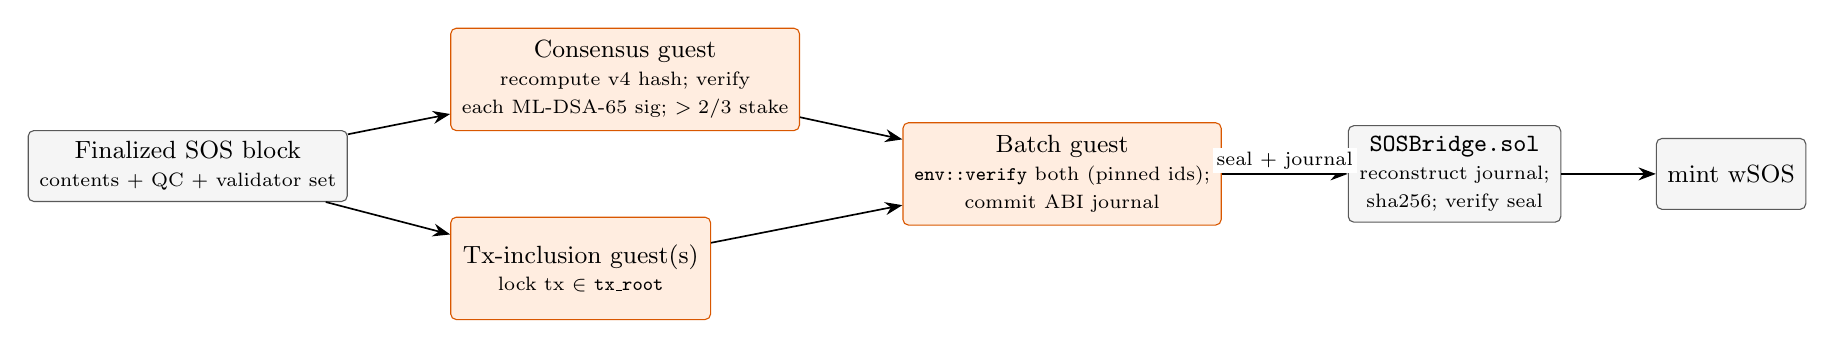
\begin{tikzpicture}[node distance=8mm and 13mm]
  \node[sbox, align=center] (block) {Finalized SOS block\\[-1pt]{\scriptsize contents + QC + validator set}};
  \node[guest, right=13mm of block, yshift=11mm] (cg) {Consensus guest\\[-1pt]{\scriptsize recompute v4 hash; verify}\\[-1pt]{\scriptsize each \mldsa{} sig; $>2/3$ stake}};
  \node[guest, right=13mm of block, yshift=-13mm] (ig) {Tx-inclusion guest(s)\\[-1pt]{\scriptsize lock tx $\in$ \code{tx\_root}}};
  \node[guest, right=13mm of cg, yshift=-12mm] (bg) {Batch guest\\[-1pt]{\scriptsize \code{env::verify} both (pinned ids);}\\[-1pt]{\scriptsize commit ABI journal}};
  \node[sbox, right=16mm of bg, align=center] (sol) {\code{SOSBridge.sol}\\[-1pt]{\scriptsize reconstruct journal;}\\[-1pt]{\scriptsize sha256; verify seal}};
  \node[sbox, right=12mm of sol, align=center] (mint) {mint wSOS};
  \draw[arr] (block) -- (cg);
  \draw[arr] (block) -- (ig);
  \draw[arr] (cg) -- (bg);
  \draw[arr] (ig) -- (bg);
  \draw[arr] (bg) -- node[el,above]{seal + journal} (sol);
  \draw[arr] (sol) -- (mint);
\end{tikzpicture}}%
\caption{SOS$\to$Ethereum by recursive STARK composition. The consensus guest
verifies a real FIPS-204 stake-weighted quorum certificate inside the proof;
the batch guest folds it with the inclusion proofs under pinned sub-program
identities and commits the exact ABI bytes the contract re-derives. Only the
final seal verification is pre-quantum.}
\label{fig:bridge}
\end{figure}

\subsubsection{The consensus guest}
\label{sec:consensus-guest}

Input: the v4 block-hash components (Construction~\ref{con:blockhash}), the
signed \code{block\_hash}, the QC round, the QC as (validator index, raw
signature) pairs, the validator set as (1952-byte key, effective stake)
pairs in canonical order, the claimed validator-set hash, epoch, and chain
id. The guest, in order:

\begin{enumerate}[leftmargin=1.6em]
\item recomputes \code{block\_hash} $=$ \code{block\_hash\_v4}$(\ldots)$ from
  the components and asserts equality with the signed hash --- binding
  \code{tx\_root}, \code{chain\_id}, the epoch, \emph{and the validator-set
  hash} to the hash the quorum actually signed;
\item recomputes the validator-set hash from the supplied set
  (Construction~\ref{con:valsethash}) and asserts it equals the bound value
  --- anchoring the very keys used in step 4 to the signed block, so a
  malicious prover cannot substitute its own set;
\item reconstructs the 58-byte precommit preimage
  (Construction~\ref{con:vote});
\item verifies each QC signature with FIPS-204 \mldsa{} (the same
  pure-Rust verifier as the node, compiled to rv32im), summing the effective
  stake of distinct valid signers, skipping (never trusting) malformed
  entries;
\item asserts the strict stake quorum $3 \cdot \mathrm{signed} >
  2 \cdot \mathrm{total}$;
\item commits $(\code{block\_hash}, h, \code{tx\_root}, V, e,
  \code{chain\_id}, \ldots)$ as its journal (field layout in
  Figure~\ref{fig:wire-guest-journals}).
\end{enumerate}

Each in-guest \mldsa{} verification costs $\approx 5.87$M cycles unaccelerated
($\approx 3.67$M with the Keccak accelerator of Section~\ref{sec:accel});
the guest's verification semantics are bit-compatible with the node's by
construction (same library, same preimage builder), which is itself pinned
by cross tests.

\subsubsection{The transaction-inclusion guest}
\label{sec:inclusion-guest}

Proves that a bridge-lock transaction is a leaf of the block's
\code{tx\_root}: it computes $\mathit{txid} =
H_{\code{bqp:txid:v1}}(\mathit{tx\_bytes})$, folds the supplied Merkle path
with the sorted-pair node hash
$H_{\code{bqp:merkle:v1}}(\min(a,b) \concat \max(a,b))$, asserts the result
equals the expected \code{tx\_root}, parses the lock's fixed-offset fields
(32-byte \code{lock\_id}, 20-byte Ethereum recipient, 8-byte amount, 8-byte
relay fee), and commits them with the root. One receipt per lock; a batch
carries many.

\subsubsection{The batch guest and pinned recursion}
\label{sec:batch-guest}

The batch guest recursively verifies one consensus receipt and $n$ inclusion
receipts via \code{env::verify}, then binds them: each inclusion journal's
\code{tx\_root} must equal the consensus journal's \code{tx\_root}, and the
consensus journal's validator-set hash must equal the value the Ethereum
contract is known to track. Crucially, the image ids of the two sub-programs
are \emph{compile-time constants inside the batch guest}, not host inputs: a
host-chosen sub-id would let an untrusted prover substitute an arbitrary
program for the audited consensus checker. Because the constants are baked
into the batch guest's binary, the batch guest's own image id ---
and therefore the immutable \code{batchGuestImageId} the contract was
deployed with --- \emph{transitively commits to exactly these sub-programs};
CI tests assert the pinned constants equal the freshly built sub-guest ids,
so any drift fails the build rather than silently changing the statement
being proven.

\subsubsection{The ABI journal}
\label{sec:journal}

The batch guest commits, as raw journal bytes, exactly
\[
\mathrm{abi.encode}\big(\code{blockHash},\ \code{height},\
\code{validatorSetHash},\ \code{epoch},\ \code{chainId},\
\code{operations[]}\big),
\]
where each operation is the static tuple
$(\code{lockId}, \code{ethRecipient}, \code{amount}, \code{relayFee})$.
The encoder is a dependency-free Rust function whose output is asserted
byte-identical to Solidity's \code{abi.encode} by a cross-language test
(against a Foundry-generated reference vector); the layout is
6 head words (with the dynamic-array offset in the sixth), then the array
length, then $4 \times 32$ bytes per operation
(Appendix~\ref{app:layouts}, Figure~\ref{fig:wire-journal}).

\subsubsection{The on-chain verifier}
\label{sec:contract}

\code{SOSBridge.processDeposits} receives the seal and the journal's
\emph{fields} (never a digest): it re-encodes
$\mathrm{abi.encode}(\ldots)$ from its own calldata, derives
$\mathrm{sha256}(\mathrm{journal})$ on-chain, and calls the RISC Zero
verifier contract with (seal, pinned \code{batchGuestImageId}, derived
digest). Because the digest is derived rather than supplied, the calldata
fields are \emph{bound} to the verified proof: any tampering changes the
digest and the verification reverts. The contract then enforces, in order:
the batch is non-empty; the proven \code{chainId} equals the immutable
expected chain id; the proven validator-set hash equals the tracked one; the
block height does not regress (same-height batches are allowed for multiple
locks in one SOS block); per-\code{lockId} replay protection; and
$\code{relayFee} \le \code{amount}$. It mints
$\code{amount} - \code{relayFee}$ wSOS to the recipient and the fee to the
submitting relayer --- which is what makes relaying permissionless: a relayer
can neither forge nor alter a withdrawal, only carry a valid one. The
burn-for-withdrawal path records burns in contract storage for the reverse
direction.

\subsection{Soundness}
\label{sec:bridge-soundness}

\begin{theorem}[Bridge soundness, SOS$\to$Ethereum]
\label{thm:bridge}
Under Assumptions~\ref{ass:mldsa}, \ref{ass:hash}, \ref{ass:stark}, and the
soundness of the Groth16 wrap at the Ethereum boundary, any
\code{processDeposits} call that mints wSOS corresponds to bridge-lock
transactions included in an SOS block that obtained a strictly
$>\!2/3$-stake \mldsa{} precommit quorum from the validator set whose hash
the contract tracks, on the expected chain, in the claimed epoch.
\end{theorem}

\begin{proof}[Proof sketch]
Minting requires the verifier contract to accept (seal,
\code{batchGuestImageId}, digest) with the digest derived on-chain from the
calldata. Acceptance under the wrap's soundness implies a valid receipt for
the batch program with journal bytes equal to the calldata encoding ---
fields cannot be detached from the proof. The batch program (fixed by the
immutable image id) accepts only if \code{env::verify} discharged receipts
for the \emph{pinned} consensus and inclusion programs
(Assumption~\ref{ass:stark} makes fabricating either infeasible) with
matching \code{tx\_root}s and the tracked validator-set hash. The consensus
program accepts only if the recomputed v4 hash equals the signed hash (so
\code{tx\_root}, \code{chainId}, epoch, and the set hash are the signed
ones, Assumption~\ref{ass:hash} for collisions) and only if distinct
validators of the bound set, holding strictly more than $2/3$ of its stake,
produced valid \mldsa{} signatures over the 58-byte precommit preimage
(Assumption~\ref{ass:mldsa}). The inclusion program accepts only leaves of
the bound \code{tx\_root} (Assumption~\ref{ass:hash}). Composing: a mint
reduces to a real finalized SOS block and real included locks, or to a break
of one of the stated assumptions. The residual trust is therefore exactly
SOS's own honest-stake assumption (Assumption~\ref{ass:byz}) plus the
enumerated Ethereum-side verifier --- no bridge-specific committee exists to
compromise.
\end{proof}

Replay is excluded at three layers: \code{chain\_id} inside the signed hash
(cross-chain), the epoch inside the signed hash (cross-validator-set
generations), and \code{lockId}/height monotonicity in the contract
(cross-batch).

\subsection{The non-PQ boundary at Ethereum}
\label{sec:nonpq}

Everything on the SOS side of Figure~\ref{fig:bridge} is hash-based STARK
verification of \mldsa{} signatures over \sha{} preimages --- post-quantum
throughout. Ethereum, however, cannot affordably verify a FRI transcript
on-chain, so the relayer wraps the final STARK receipt into a Groth16 proof
over BN254 \cite{groth16} --- the standard RISC Zero on-chain pattern ---
and \emph{that} pairing-based seal is what the contract checks. This is the
first of the two enumerated external-chain compatibility modules of
Definition~\ref{def:boundary}. Its failure domain is precisely scoped: a
quantum (or classical) break of the wrap forges \emph{wSOS on Ethereum};
it cannot touch the SOS ledger, whose own verifiers never accept wrapped
receipts. Symmetrically, SOS-internal verifiers are required to reject
non-STARK receipt kinds; hardening this rejection explicitly everywhere is
tracked as an open item in Section~\ref{sec:tcb}.

\subsection{Ethereum $\to$ SOS}
\label{sec:eth-to-sos}

The reverse direction mints native SOS against a proven burn of wSOS. The
construction is an Ethereum light client \emph{inside a guest}
\cite{altair2021}: a proof that (i) the Ethereum sync committee's BLS12-381
aggregate signature (the second enumerated non-PQ module) covers a recent
beacon-chain header with a $\ge 2/3$ supermajority; (ii) the header whose
execution state holds the burn is the \emph{finalized} checkpoint under that
signed header --- reorg safety, so a head that later reorganizes cannot have
released --- proven by a finality Merkle branch; and (iii) the burn record
exists in the bridge contract's storage, via Merkle--Patricia trie account and
storage proofs (keccak256) against the execution state root, with the burn's
amount and SOS recipient hash \emph{extracted from the proven storage words}
(never trusted from an input). The burn's parameters are committed in the
journal; the SOS node verifies the receipt and credits the recipient, debiting
\code{bridge\_locked}.

Status \statusI{}: the guest performs \emph{real} BLS12-381 aggregate
signature verification of the sync committee over the signed header --- a
$\ge 2/3$-of-$512$ supermajority, not a participation-count or length check ---
together with the finalized-header, execution-payload, and MPT account/storage
proofs that \emph{extract} the released amount and recipient. This has been
demonstrated end-to-end against live Ethereum Sepolia: a wSOS burn on Sepolia
was proven by a GPU-generated STARK and verified on-node, after which the node
minted the released amount from \code{bridge\_locked}, with the locked-backing
accounting conserved (a release debits exactly what it mints). The eth-burn
verifier and the release mint are \emph{enabled by default} (the default
\code{privacy-stark} feature); a node built without that feature --- and
without the opt-in \code{insecure-bridge} feature --- fail-closes and refuses
to mint, so no unproven path can create SOS. Each proof is anchored to a
\emph{per-node-deterministic} trusted set of sync-committee roots (seeded at
genesis from a pinned constant and extended by proven Altair committee
rotations applied identically on every node, and persisted) and to the pinned
bridge address. The trusted committee-root set is folded into
\code{app\_hash}, so nodes that disagree on the reverse-bridge trust anchor
cannot continue with the same application hash. The remaining gap to
\statusV{} is exercising this path under the multi-node load/chaos harness.

\paragraph{Deposit-lock lifecycle.} A SOS-side deposit lock, which backs minted
wSOS, is \emph{final}: the locked value returns to its owner only through the
reverse burn-and-release path above --- burning the wSOS on Ethereum and
proving it --- never through an automatic on-chain timeout. A time-bounded
owner-reclaim was analyzed and \emph{deferred}: a fixed block-count reclaim
threshold cannot be made reliably exclusive with the Ethereum-side claim on a
sub-second-block chain unless the chain enforces a block-time floor or the
deposit proof commits the chain-tip height; both are noted as future
enhancements. The paper therefore describes no auto-refund, because none ships
today.

\subsection{Validator-set evolution}
\label{sec:valset-evolution}

The contract tracks one validator-set hash; following its evolution is the
classical weak-subjectivity problem of proof-of-stake light clients
\cite{weaksubj2014}. Rotating it requires an \emph{epoch-transition proof}
--- a guest proving that set $V_{e+1}$ is the legitimate successor of $V_e$
under SOS's staking rules --- with the same journal-reconstruction
discipline as deposits. The valset-transition guest and
\code{updateValidatorSet} entrypoint are implemented and image-id pinned, so
the on-chain path is no longer intentionally fail-closed. \statusI{} The public
rehearsal completed this lifecycle: a V0 deposit was processed, a canonical
receipt proved the transition from epoch~7 hash
\code{2d0c961c\ldots c1b1e} to epoch~226 hash
\code{59024532\ldots 4de2}, and Sepolia transaction
\code{1ee99775\ldots b93ff} rotated the contract. A new V1 deposit was then
processed in transaction \code{491ddd6e\ldots 5f2c}; transition replay, V1 lock
replay, and a stale-V0 deposit all reverted. Wrong-overlap inputs remain covered
by the guest/host negative suite. The PCF epoch chain of
Section~\ref{sec:pcf} (whose checkpoints already bind
\code{validator\_set\_hash} per epoch and chain contiguously) is the intended
long-term substrate for this proof. Mainnet still needs automated churn
campaigns and a deployment-domain migration protocol; these are catalogued in
Section~\ref{sec:tcb}.

\subsection{Weak subjectivity on the SOS side}
\label{sec:light-client-assumptions}

Light clients verifying finality without full state face a complementary
weak-subjectivity problem on the SOS side: an exited validator, slashed or
naturally unbonded, is no longer in the active set and therefore not part of
the quorum denominator, but may sign forks of the chain's history at heights
where they were still bonded. A light client must therefore commit to a
sufficiently recent \emph{checkpoint} (a finalized block header and its QC) to
ensure that the validator set cannot have been substituted without the client's
knowledge. The protocol's active-set epoch is only 100 blocks and is an
implementation cadence, \emph{not} by itself a defensible maximum-offline or
weak-subjectivity period. The public testnet therefore requires mobile wallets
and explorers to re-sync the validator set and quorum denominator against live
peers; it does not claim that one epoch supplies an hours-long trust window. For
the longer-term PCF certificate of Section~\ref{sec:pcf}, the epoch-chain proof
embeds validator-set transitions contiguously, allowing a client to verify them
with one STARK artifact per segment. Before mainnet, an operational policy must
fix independently distributed checkpoint sources, publication cadence,
maximum offline time derived from unbonding and evidence windows, restart
behavior, and user-visible bootstrap rules. Until that policy and consumption
path are live, clients rely on explicit recent-checkpoint discipline.

\subsection{Implementation status}
\label{sec:bridge-status}

What exists and is tested \statusI{}: all three guests (consensus with
FIPS-204 verification, inclusion, batch) build reproducibly and are embedded
with pinned image ids and drift tests; the recursive composition round-trips
end-to-end in host tests (a real $>2/3$-stake \mldsa{} quorum proven inside
the consensus guest; sub-quorum, tampered-\code{tx\_root}, and wrong-set
inputs rejected); the ABI encoder is cross-checked against Solidity; and the
hardened \code{SOSBridge} contract passes its Foundry suite including
digest-binding, tamper, replay, and fee-bound tests.

What has been demonstrated on a live network \statusI{}: the full relayer
pipeline fetches real (block, QC, validator set, Merkle path) data from a node,
composes the three proofs, wraps the result to a Groth16 seal, and submits it
against a \code{SOSBridge} deployment pinned to the batch image id on Ethereum
Sepolia. The active TVL-limited contract is
\code{0x862Bc5c5\ldots 79e93}, deployed at Sepolia block~11244918 with a
10,000-SOS global outstanding cap and 1,000-SOS per-deposit cap, mirrored by
SOS consensus. A 1,000,000-sat V0 lock at SOS height~1640 was processed in
transaction \code{581b1105\ldots a22fc}; the reverse direction then burned
500,000 sats in transaction \code{db13a1d8\ldots 4c4be}, and a 224,442-byte
real succinct STARK receipt proved Ethereum finality before every SOS validator
persisted the release. The public V0-to-V1 rehearsal subsequently rotated the
contract and processed a 200,000-sat V1 lock at SOS height~26257. At the end of
the rehearsal the contract reported 1,200,000 sats minted, 500,000 burned, and
700,000 outstanding. Deposit and transition replays were rejected, stale-V0
proofs failed after rotation, burn replay was idempotent, restart rebuilt the
bridge RPC view, and a relayer with empty local state reconciled all operations
from chain truth without duplicate submission. An unattended relayer,
sync-committee-root maintainer, and fail-closed monitor remain live; the monitor
compares the finalized SOS validator-set hash with the contract on every run.
The repository's dated E2E record preserves the full image ids and transaction
identifiers.

What remains \statusP{}: the full cross-chain pipeline has not yet been run as
a sustained bridge/privacy workload inside the multi-node fault harness; the
tested fresh-cutover image policy still needs a consensus-defined
\code{bridgeDomain} and activation/drain protocol for mainnet; the beta caps
need an externally reviewed economic relation to slashable stake before they
can be raised; and validators, relayers, provers, monitoring, and alert ownership
need independent operators and failure domains. The SOS-side timeout refund
path remains disabled until claim/refund exclusivity is proven under the
chain's timing and finality assumptions
(Section~\ref{sec:valset-evolution}). The current Foundry and live negative
checks still need promotion to reproducible release CI and independent review.
Theorem~\ref{thm:bridge} applies to this implemented and demonstrated
construction under those launch gates.

% ============================================================================
\section{Scalability: Proof-Carrying Finality and the Native ML-DSA AIR}
\label{sec:scalability}
% ============================================================================

This section treats the central scalability constraint of a post-quantum BFT
chain quantitatively, reports the negative results that pruned the design
space, and presents the chosen program: a bounded-validator launch, an
epoch-checkpoint finality certificate that reuses the consensus STARK
(\emph{Proof-Carrying Finality}, PCF), a measured zkVM acceleration stack,
and a native ML-DSA verification AIR as the research path to an unbounded
validator set. All numbers marked measured were produced on the project's
prover lab (4$\times$RTX~3090, real proving mode) or its WSL executor (cycle
counts), and are reproducible from the repository.

\subsection{The problem, quantified}
\label{sec:qc-problem}

A quorum certificate carries one 3309-byte \mldsa{} signature per signer, and
the bridge's consensus guest re-verifies each in-zkVM at
$\approx 5.87$M cycles. Both grow linearly in the signer count $N$
(Table~\ref{tab:qcsize}):

\begin{table}[ht]\centering
\adjustbox{max width=\textwidth}{%
\begin{tabular}{@{}rrr@{}}
\toprule
$N$ signers & QC signature bytes & in-zkVM verify cycles \\
\midrule
67   & $\approx 0.22$ MB & $\approx 0.39 \times 10^9$ \\
128  & $\approx 0.42$ MB & $\approx 0.75 \times 10^9$ \\
256  & $\approx 0.85$ MB & $\approx 1.50 \times 10^9$ \\
1000 & $\approx 3.31$ MB & $\approx 5.87 \times 10^9$ \\
\bottomrule
\end{tabular}}
\caption{Linear growth of the post-quantum QC. The linear term propagates
into block size (4 MiB ceiling), gossip, light-client bandwidth,
bridge-prover cost, archive growth, and catch-up latency.}
\label{tab:qcsize}
\end{table}

Pre-quantum chains hide this with BLS aggregation: hundreds of signatures
over one message compress to 96 bytes and one pairing check --- which is
exactly the primitive the post-quantum setting removes. The problem is to
recover an aggregation-\emph{like} property without leaving the PQ regime,
under the project's non-negotiables: full PQ internally, privacy untouched,
the bridge non-custodial and proof-authorized, the staking set unbounded
economically, and BFT
safety under Assumption~\ref{ass:byz}.

\subsection{Negative results}
\label{sec:negative}

Three candidate routes were investigated to a decision and rejected; we
record them because the reasons are load-bearing for the chosen design.

\paragraph{(a) Stake-weighted committee sampling does not preserve the
$1/3$ margin with un-aggregated signatures.} Sampling a committee of
expected size $K$ by public hash-sortition over the on-chain beacon is
attractive (no new cryptography; the QC becomes $O(K)$). But sizing $K$ so
that $\Pr[\mathrm{Bin}(K, \beta) \ge K/3] \le 2^{-40}$ --- the probability a
committee over-represents Byzantine stake to the safety threshold --- gives,
by exact binomial computation: $\beta = 0.10 \Rightarrow K = 124$;
$\beta = 0.15 \Rightarrow 241$; $\beta = 0.20 \Rightarrow 508$;
$\beta = 0.25 \Rightarrow 1432$; $\beta = 0.30 \Rightarrow 9601$; and
$K \to \infty$ as $\beta \to 1/3$. With $\approx 7$\,KB per signer, only the
$\beta \le 0.10$ row fits a 1\,MiB block budget --- i.e.\ sampling with
plain \mldsa{} forces a choice between gutting the Byzantine margin
(operating assumption ``$\ge 90\%$ honest stake'') and committees that do
not fit a block. Honest-offline validators inflate the effective $\beta$
further. Committee sampling is therefore not a substitute for the full-set
QC at SOS's stated margin.

\paragraph{(b) Lattice synchronized multi-signatures are not adoptable
today.} Squirrel \cite{squirrel2022}, Chipmunk \cite{chipmunk2023}, and
Lemur \cite{lemur2026} aggregate many same-slot lattice signatures
sub-linearly ($\approx$150--200\,KB for thousands of signers) and would
restore the full margin with one aggregate verification. The blockers are
maturity, not feasibility: re-evaluation of Chipmunk's shipped parameters
places its concrete security far below the claimed level; Lemur is weeks
old, rests on a new assumption (Dual-Hint-MLWE), and requires gigabytes of
key-evolving signer state; all are non-FIPS with research-grade
implementations; and their NTT-heavy verification is the worst cost profile
for in-zkVM re-verification (the zkVM accelerates hashes, not lattice
arithmetic). Verdict: track for 2027+; do not place unaudited 2026 lattice
aggregation on the consensus critical path of a chain whose premise is
conservative cryptography.

\paragraph{(c) Algebraic batch verification of distinct-signer ML-DSA is
structurally unavailable.} ML-DSA's verification is
commitment-recoverable Fiat--Shamir ending in a per-signer hash equality
with a key-prefixed challenge, with non-linear \code{Decompose}/\code{UseHint}
rounding and non-algebraic $\infty$-norm checks; a random-linear-combination
batch across \emph{distinct} keys has no sound formulation (published
batching results are same-signer only). Total verification work is
$\Theta(N)$; all available gains are per-verification cost and per-\emph{key}
amortization --- which is what the acceleration stack below pursues.

\subsection{Launch posture: bounded active set}
\label{sec:bounded}

Given (a)--(c), SOS launches with a bounded \emph{active} validator set
($N \le 128$), the full raw QC in every block, plain FIPS-204 \mldsa{}, and
the complete $<\!1/3$ Byzantine margin --- zero new cryptographic
assumptions, QC within the block budget, and the validator-set binding of
Construction~\ref{con:blockhash} already in place. Delegation keeps economic
participation unbounded while the signing set is bounded; the linear-QC
constraint binds above roughly 150--200 validators and is thus a scaling
road-map item rather than a launch blocker. The two tracks below are the
road map.

\subsection{Proof-Carrying Finality (PCF)}
\label{sec:pcf}

The consensus guest of Section~\ref{sec:consensus-guest} already verifies a
full stake-weighted \mldsa{} quorum inside a hash-based STARK. PCF's
observation is that this proof, built for the bridge, is \emph{the} portable
finality object the rest of the system wants: one succinct receipt can
replace $N$ raw signatures for every consumer that is not the real-time
consensus path itself.

\begin{construction}[Epoch-checkpoint certificate]
\label{con:pcf}
\statusI{} The epoch-checkpoint guest takes a contiguous, height-ordered run
of blocks $\{(h_i, \mathrm{QC}_i)\}$ under one fixed validator set and
proves, for \emph{every} block in the run, exactly the per-block statement
of Section~\ref{sec:consensus-guest} (v4 hash recomputation, per-signature
FIPS-204 verification, strict stake quorum), with two structural additions:
heights must be strictly consecutive, and the journal commits
\[
\begin{aligned}
\big(&\code{chain\_id}, e, V, h_{\mathrm{first}}, h_{\mathrm{last}}, \\
  &\code{block\_hash}_{\mathrm{first}}, \code{block\_hash}_{\mathrm{last}}, C_{\mathrm{blocks}}, \mathit{count}\big),
\end{aligned}
\]
where $C_{\mathrm{blocks}}$ is a domain-separated \sha{} hash chain over
each block's $(h, \code{block\_hash}, \code{tx\_root})$
(tags \code{sos:epoch-blocks:v1} / \code{sos:epoch-blocks:step}; journal
field layout in Figure~\ref{fig:wire-guest-journals}). A consumer
authenticates \emph{any interior block} --- and its \code{tx\_root}, for a
transaction-inclusion proof --- against the single receipt, and chains
consecutive checkpoints by
$h^{\mathrm{next}}_{\mathrm{first}} = h^{\mathrm{prev}}_{\mathrm{last}} + 1$.
A companion \emph{compose} guest recursively verifies $G$ shard receipts
(pinned to the canonical epoch image id) and stitches contiguous ranges into
one certificate, enabling parallel proving across GPUs.
\end{construction}

Consumers: mobile light clients check one constant-size STARK per epoch
instead of $N$ \mldsa{} signatures per block; syncing full nodes replace
$N$ verifications per block during catch-up; and the bridge shares the same
artifact, aligning bridge security with consensus security. The chain-segment
property --- at most one quorum block per height, each building on the
previous --- holds because consensus safety (Theorem~\ref{thm:safety})
guarantees it for quorum-certified blocks.

Honest scoping, per the project's own review: PCF is finality
\emph{compression}, not validator scaling --- the block still carries the
raw QC, which remains authoritative for real-time finalization (the
certificate trails by proving latency and ships as an epoch checkpoint, in
the spirit of Algorand's state proofs \cite{compactcerts2020}, never as a
gate: a missing certificate withholds a reward, never halts the chain).
The $\approx$150--200-validator ceiling stands until the per-verification
cost falls (Section~\ref{sec:accel} and the native-AIR program of
Section~\ref{sec:airtrack}). Before the
certificate can become consensus-law for any consumer, identified gaps must
close: an image-id rotation protocol (the on-chain id is immutable today),
the epoch-transition guest of Section~\ref{sec:valset-evolution}, explicit
rejection of wrapped (non-STARK) receipts by internal verifiers, and a
differential-check/disable switch so a hypothetical guest soundness bug is
a recoverable liveness event rather than a forgeable finality certificate.
Measured: a 4-block, 4-validator checkpoint proves in $\approx 76$\,s on one
lab GPU; sharded composition across 2 GPUs achieves $1.91\times$
(near-ideal) scaling on the verify-dominated portion.

\subsection{Measured acceleration of in-zkVM ML-DSA verification}
\label{sec:accel}

The lever that shortens PCF epochs --- and eventually unbinds $N$ --- is the
per-verification zkVM cost. Table~\ref{tab:accel} summarizes the stack with
measured results (4$\times$RTX 3090 lab, real proving mode unless noted).

\begin{table}[ht]\centering
\adjustbox{max width=\textwidth}{%
\small
\begin{tabular}{@{}llll@{}}
\toprule
\textbf{Lever} & \textbf{Mechanism} & \textbf{Measured effect} & \textbf{Status} \\
\midrule
S1 Keccak accelerator & route Keccak-$f[1600]$ to the & 1 verify: $12.55 \to 9.53$\,s wall & \statusM{} \\
 & dedicated zkVM circuit & ($1.32\times$); cycles $6.42 \to 3.67$M & \\
S2 key-decode cache & decode each validator key once & $-39\%$ wall at $B{=}8$ blocks/epoch & \statusM{} \\
 & per epoch (PCF guest) & ($54.0 \to 32.8$\,s); $43.9\%$ of & \\
 & & per-verify work eliminable as $B \to \infty$ & \\
S3 modular-product precompile & NTT as a checked big-integer & --- & \statusR{} \\
 & identity in a native circuit & & \\
S4 lean FIPS-204 decode path & replace the generic library tail & --- & \statusR{} \\
S5 native ML-DSA AIR & prove verification in a dedicated & Section~\ref{sec:airtrack} & \statusM{} \\
 & circuit, not RISC-V emulation & & \\
S6 shard composition & prove epoch shards in parallel, & $1.91\times$ on 2 GPUs (near-ideal) & \statusM{} \\
 & recursively compose & & \\
\bottomrule
\end{tabular}}
\caption{The acceleration stack. Dashes: not yet measured.}
\label{tab:accel}
\end{table}

Two methodological points from these measurements are worth recording.
First, \emph{cycle counts overstate wall-clock gains for levers that move
work} into a dedicated circuit rather than eliminating it: S1's $-43\%$
rv32im cycles delivered $-24\%$ wall-clock, because the accelerated
permutations still cost proving time in their own circuit. Levers that
\emph{eliminate} work track cycles faithfully or better: S2's wall-clock
reduction ($-39\%$) exceeded its cycle reduction ($-32\%$) in the
S1-stacked configuration, and matched it within $0.1$ percentage points in
the software-Keccak configuration. Second, the headline S2 percentages are
\emph{asymptotes} ($B \to \infty$); the delivered per-block saving at the
measured $B = 8$ is $\approx 38\%$. S2 amortizes per-\emph{key} work across
an epoch and does not touch the per-message verification, so it shortens
epochs but does not raise the validator ceiling.

\subsection{The native ML-DSA AIR (S5): summary of the measured verdict}
\label{sec:airtrack-summary}

\statusM{} The research endgame of the acceleration stack is to stop paying
RISC-V emulation overhead for the algebra entirely: express FIPS-204
verification as a dedicated AIR, prove a \emph{batch} of $K$ verifications
in one transparent FRI STARK, and have a thin zkVM guest verify that one
batched proof in software --- preserving \code{env::verify}, the recursion
pipeline, and the on-chain interface unchanged (\emph{wrap, not replace}).
The project gated this track on two pre-registered kill-criteria; both are
now retired with measured data: (1) the full 8-layer forward NTT proves
natively in $\approx 0.20$\,s, about $2\%$ of the $9.53$\,s post-S1 zkVM
verification budget (kill threshold: one NTT above $\sim$10\% of a full
zkVM verify); and (2) the in-guest software verification of the native
proof costs $174.1$M cycles after two measured accelerations, a crossover
of $K^\ast \approx 47.4$ direct verifications --- clearing the realistic
67--128 signatures per quorum certificate (kill threshold: failing to clear
that range). Because this result is one of the paper's central
contributions --- and because its soundness caveats deserve the same level
of detail as its wins --- the architecture, the gadget-level soundness
arguments, the in-guest verifier, the measured data, and the remaining
engineering program are developed in the dedicated
Section~\ref{sec:airtrack}.

% ============================================================================
\section{A Native FIPS-204 Verification AIR: Wrap, Not Replace}
\label{sec:airtrack}
% ============================================================================
% Grounding (code + measurements):
%   docs/SCALABILITY.md (S5 verdict, M0/M1/M2 measured numbers, adversarial
%     review riders, remaining-program estimate);
%   crates/sos-air-spike/src/lib.rs (M0 mod-q gadget, constraint system,
%     soundness argument, forgery tests, FRI parameters at 144 bits);
%   crates/sos-air-spike/src/ntt.rs (M1 forward-NTT AIR, trace/schedule/
%     constraints, dual-oracle KATs);
%   crates/sos-air-verify/air-core/src/lib.rs (no_std AIR copies, GuestInput/
%     GuestJournal, journal_publics_hash, M1-pp preprocessed variant);
%   crates/sos-air-verify/guest/src/main.rs (in-guest verifier, V_fri cycle
%     split, in-guest VK derivation = the lever-B soundness crux);
%   crates/sos-air-verify/vendor/tiny-keccak-risc0/src/keccakf.rs (lever A:
%     free-function keccakf routed to risc0_keccak_update under cfg(zkvm)).

\statusM{} This section develops the S5 track of Table~\ref{tab:accel} in
full: a native AIR (algebraic intermediate representation) that proves
\mldsa{} verification arithmetic in a dedicated transparent-FRI STARK
\emph{outside} the zkVM, and a thin zkVM guest that verifies that native
proof \emph{inside} the zkVM and journal-commits the result --- so that
every existing consumer of finality proofs (the PCF epoch certificate, the
bridge batch recursion, the on-chain verifier) is untouched. One status
statement governs everything that follows: \emph{this is a measured
prototype on a research track}. The constraint systems, the soundness
arguments, and every number in this section exist in the repository and
were measured as described; nothing in this section is on the live
block-validation or bridge path, and Section~\ref{sec:air-program} states
the program --- and its honest cost --- that separates the prototype from
consensus-law deployment.

\subsection{Problem and architecture}
\label{sec:air-arch}

Sections~\ref{sec:qc-problem}--\ref{sec:accel} establish the cost shape:
every consumer that re-verifies SOS finality \emph{inside a proof} pays
$\approx 3.67$M zkVM cycles per \mldsa{} signature at the post-S1 baseline,
because FIPS-204 verification --- NTTs, modular arithmetic, SHAKE --- is
being emulated instruction-by-instruction as rv32im inside the zkVM's
universal execution circuit, and because algebraic batching across distinct
signers is structurally unavailable (Section~\ref{sec:negative}c). The
emulation overhead, not the arithmetic itself, dominates: the same
verification algebra, expressed directly as AIR constraints over a small
prime field, is orders of magnitude cheaper to prove. The native-AIR
program therefore moves the algebra into a dedicated circuit
(Figure~\ref{fig:air-pipeline}):

\begin{enumerate}[leftmargin=1.6em]
\item a \emph{native prover}, off-zkVM, proves a batch of $K$ FIPS-204
  verifications in one Plonky3 \cite{plonky3} uni-STARK --- a transparent,
  hash-based FRI \cite{fri2018} proof with keccak-f[1600] Merkle
  commitments \cite{fips202}, no trusted setup, and no cryptographic
  assumption beyond Assumption~\ref{ass:stark};
\item a \emph{thin zkVM guest} verifies that one native proof in software
  (cost: $V_{\mathrm{fri}}$ cycles, the make-or-break quantity of
  Section~\ref{sec:air-guest}) and commits to its journal \emph{which}
  statement was verified;
\item everything downstream is unchanged: the guest's receipt enters the
  same \code{env::verify} recursion, image-id pinning, and (for the bridge)
  Groth16 wrap as today. The verification \emph{semantics} --- unmodified
  FIPS-204, bit-exact against the reference implementation --- are
  preserved by construction and pinned by known-answer tests.
\end{enumerate}

\begin{figure}[ht]\centering
\adjustbox{max width=\textwidth}{%
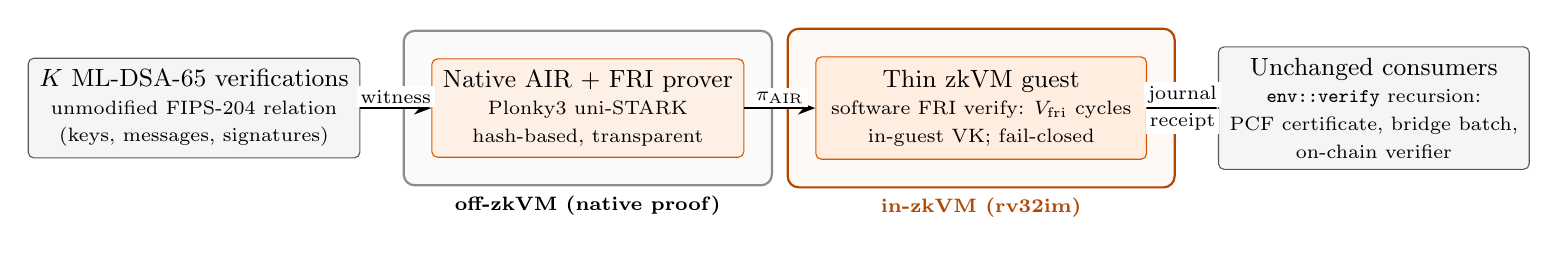
\begin{tikzpicture}[node distance=8mm and 9mm]
  \node[sbox, minimum width=31mm] (stmt) {$K$ \mldsa{} verifications\\[-1pt]{\scriptsize unmodified FIPS-204 relation}\\[-1pt]{\scriptsize (keys, messages, signatures)}};
  \node[pqbox, right=9mm of stmt, minimum width=38mm] (air) {Native AIR + FRI prover\\[-1pt]{\scriptsize Plonky3 uni-STARK}\\[-1pt]{\scriptsize hash-based, transparent}};
  \node[guest, right=9mm of air, minimum width=42mm] (g) {Thin zkVM guest\\[-1pt]{\scriptsize software FRI verify: $V_{\mathrm{fri}}$ cycles}\\[-1pt]{\scriptsize in-guest VK; fail-closed}};
  \node[sbox, right=9mm of g, minimum width=37mm] (down) {Unchanged consumers\\[-1pt]{\scriptsize \code{env::verify} recursion:}\\[-1pt]{\scriptsize PCF certificate, bridge batch,}\\[-1pt]{\scriptsize on-chain verifier}};
  \draw[arr] (stmt) -- node[el,above]{witness} (air);
  \draw[arr] (air) -- node[el,above]{$\pi_{\mathrm{AIR}}$} (g);
  \draw[arr] (g) -- node[el,above]{journal} node[el,below]{receipt} (down);
  \begin{scope}[on background layer]
    \node[draw=black!45, thick, rounded corners, fill=black!2, fit=(air),
          inner sep=3.5mm,
          label={[font=\scriptsize\bfseries]below:off-zkVM (native proof)}] {};
    \node[draw=sosorange!70!black, thick, rounded corners, fill=sosorange!4, fit=(g),
          inner sep=3.5mm,
          label={[font=\scriptsize\bfseries, text=sosorange!70!black]below:in-zkVM (rv32im)}] {};
  \end{scope}
\end{tikzpicture}}%
\caption{Wrap, not replace. A native transparent-FRI AIR proves the FIPS-204
verification arithmetic off-zkVM; a thin RISC Zero guest verifies \emph{that}
proof in software in-zkVM and journal-commits the result; the recursion
pipeline and the on-chain interface are untouched. The AIR path wins when the
batch size $K$ exceeds the crossover $K^\ast = V_{\mathrm{fri}} / 3.67\mathrm{M}$
(Section~\ref{sec:air-guest}).}
\label{fig:air-pipeline}
\end{figure}

Two framework decisions are part of the record. \emph{Toolkit:} Plonky3 is,
to our knowledge, the only independently audited multi-tenant AIR toolkit
\cite{plonky3,plonky3audit2024} and ships a production keccak-f[1600] AIR
--- relevant because SHAKE is the dominant cost center of a full FIPS-204
verification (Section~\ref{sec:air-program}). \emph{Field:} the measured
prototype runs over the 64-bit Goldilocks field, where a product of two
canonical ML-DSA coefficients ($< q = 8380417 < 2^{23}$) fits in a single
field element without limb decomposition --- the fastest path to honest
numbers; the production target is BabyBear (the 31-bit field native to the
RISC Zero stack), where the same gadget requires a limb/carry decomposition
(Section~\ref{sec:air-program}). To our knowledge no bit-exact FIPS-204
verification AIR has been published: existing lattice-signature circuits
modify the scheme for arithmetization friendliness, which would break the
SOS requirement that the circuit verify exactly the signatures the
validators produce. The measurement guest commits
$\mathrm{keccak256}(\mathit{air\_id} \concat \mathit{publics} \concat
\mathit{accept})$ as its journal, binding \emph{which} statement (e.g.\
which NTT input/output pair) was verified; a production guest would commit
the per-statement results (key digest, message, validity) for the recursion
to consume.

\subsection{Proof-system instantiation and the soundness stance}
\label{sec:air-params}

The STARK configuration is deliberately boring: keccak-f[1600] sponge
hashing for Merkle commitments and the Fiat--Shamir challenger
\cite{fips202}, a two-adic FRI polynomial commitment \cite{fri2018}, a
degree-2 binomial extension field for FRI challenges ($\approx 2^{128}$
challenge space), and a query-phase proof of work. The prototype raises the
FRI query count from the upstream benchmark default to $128$ queries at
blowup factor $2$, giving
\[
\text{conjectured soundness bits} \;=\;
\underbrace{1 \cdot 128}_{\log_2(\text{blowup}) \,\cdot\, \text{queries}}
+ \underbrace{16}_{\text{grinding}} \;=\; 144 \text{ (classical)},
\qquad \approx 136 \text{ quantum-adjusted},
\]
where the quantum adjustment halves only the 16-bit grinding term (Grover),
the FRI query term being a classical list-decoding bound for which the
ethSTARK conjecture \cite{ethstark2021} assumes no quantum speedup. We state
the honesty rider attached to these parameters in the code itself: $144$ is
the \emph{conjectured} (ethSTARK) soundness on which deployed STARKs stand;
the \emph{provable} Johnson-bound soundness at this rate is far lower
($\approx 0.5$ bits per query), and a production deployment must ratify the
conjectured stance explicitly --- exactly as the existing zkVM stack already
does implicitly --- before any AIR receipt becomes consensus-law.

\subsection{The mod-$q$ gadget (M0)}
\label{sec:air-gadget}

The atom of every lattice-verification circuit is multiplication in
$\mathbb{Z}_q$, $q = 2^{23} - 2^{13} + 1 = 8380417$ (FIPS-204). The M0
prototype proves the NTT-domain pointwise product
$c_i = a_i \cdot b_i \bmod q$ for all $256$ coefficients (FIPS-204
Algorithm~45), one coefficient per trace row.

\begin{construction}[Range-checked mod-$q$ multiplication gadget]
\label{con:modq}
Let $s = 2^{23} - q = 8191$. A trace row carries value columns
$(a, b, k, r)$ and seven 23-bit decompositions: plain decompositions of
$a, b, k, r$ and \emph{shifted} decompositions of $r + s$, $a + s$,
$b + s$. The constraints, all of polynomial degree at most 2, are:
\begin{enumerate}[leftmargin=1.6em]
\item \emph{booleanity}: every bit column $\beta$ satisfies
  $\beta(\beta - 1) = 0$;
\item \emph{recomposition}: each plain decomposition satisfies
  $\sum_i \beta_i 2^i = x$ for its value column $x \in \{a, b, k, r\}$;
\item \emph{canonicity}: each shifted decomposition satisfies
  $\sum_i \beta_i 2^i = x + s$ for $x \in \{a, b, r\}$;
\item \emph{Euclidean identity}: $a \cdot b - k \cdot q - r = 0$.
\end{enumerate}
The width is $4 + 7 \times 23 = 165$ columns; the M0 trace is
$256 \times 165$.
\end{construction}

\begin{proposition}[Gadget soundness]
\label{prop:modq}
Over a prime field with $p > 2^{47}$, any row satisfying the constraints of
Construction~\ref{con:modq} has $a, b, r$ canonical (i.e.\ $< q$) and
$r = a \cdot b \bmod q$, as integers.
\end{proposition}

\begin{proof}
Constraints (1)+(2) force $a, b, k, r \in [0, 2^{23})$ as integers: each is
a sum of 23 boolean-constrained bits, and since $2^{23} < p$ the
recomposition has no field wraparound. Constraint (3) additionally forces
$x + s \in [0, 2^{23})$, i.e.\ $x \le 2^{23} - 1 - s = q - 1$, for
$x \in \{a, b, r\}$: both decompositions of each value are necessary --- the
plain one excludes ``negative'' residues $p - x$, the shifted one pins
$x < q$ --- and together they pin the unique canonical representative.
Given these ranges, $a \cdot b < 2^{46}$ and $k q + r < 2^{23} q + 2^{23}
< 2^{46} + 2^{23}$, so $|a \cdot b - k \cdot q - r| < 2^{46} + 2^{23} <
2^{47} < p$ and constraint (4) holds \emph{over the integers}, not merely
modulo $p$: $a \cdot b = k q + r$ with $0 \le r < q$, and $r$ is the unique
canonical remainder.
\end{proof}

Each clause of Proposition~\ref{prop:modq} is load-bearing, and the
prototype's adversarial review demonstrated this constructively: without
the shifted $r$-decomposition a malicious prover commits $r' = r + q$ (with
$k' = k - 1$) whenever $r < 8191$, breaking bit-exactness with FIPS-204;
without the $k$ range check, a quotient of order $2^{41}$ satisfies the
identity modulo $p$ for \emph{any} claimed remainder; and the shifted input
decompositions make the atom \emph{self-certifying} --- sound to compose
into larger circuits (the NTT butterfly) without trusting an upstream range
check. Four forgery vector classes (non-canonical remainder, non-boolean
bit, over-large quotient, non-canonical input) are maintained as negative
tests, each asserted to fail at the verifier's out-of-domain constraint
check rather than at some incidental proof-shape error. Bit-exactness is
established by a known-answer test against the reference \code{ml-dsa}
implementation --- instantiated through the \emph{identical} version-pinned
field-arithmetic monomorphization the node itself executes, so the oracle
is the deployed code, not a transcription --- with an independent integer
cross-check of the oracle. Measured \statusM{}: the $256 \times 165$ trace
proves in $\approx 5.3$\,ms on the host CPU at the 144-bit parameter set
($\approx 0.06\%$ of the $9.53$\,s post-S1 in-zkVM verification budget).

\subsection{The forward-NTT AIR (M1)}
\label{sec:air-ntt}

M1 scales the gadget to the largest single algebraic block of FIPS-204
verification: the complete 8-layer forward NTT (FIPS-204 Algorithm~41) ---
$8$ layers $\times$ $128$ butterflies $= 1024$ Cooley--Tukey butterflies in
exactly the reference implementation's loop order, with twiddles
$\zeta^{\mathrm{bitrev}_8(m)} \bmod q$, $\zeta = 1753$.

\begin{construction}[Forward-NTT AIR]
\label{con:nttair}
The trace is $2048 \times 425$: one butterfly per row, with row $r$ holding
the 256-coefficient working state \emph{before} butterfly $r$ (256
columns), the butterfly witness ($u$, $v$, the multiplication gadget's
quotient and canonical product $t = z \cdot v \bmod q$, two conditional-%
subtraction bits, and the canonical outputs $u_{\mathrm{out}} = u + t
\bmod q$, $v_{\mathrm{out}} = u - t \bmod q$; 8 columns), and seven 23-bit
decompositions instantiating the dual-decomposition discipline of
Construction~\ref{con:modq} for $t$, $u_{\mathrm{out}}$,
$v_{\mathrm{out}}$ and the quotient (161 columns). Rows $0..1023$ carry the
butterflies; row $1024$ holds the NTT output; rows $1025..2047$ are
copy-padding so the output also appears on the last row. The butterfly
\emph{schedule} --- which state pair $(j, j{+}\mathrm{len})$ a row touches,
with which twiddle --- is a public constant of FIPS-204, supplied as $513$
\emph{periodic columns} (one twiddle column and $256 + 256$ one-hot operand
indicators). The constraints (943 total, degree $\le 2$) are: booleanity;
the seven recompositions; operand extraction
($\sum_i \mathrm{PU}_i \cdot \mathit{state}_i = u$ and symmetrically for
$v$); the multiplication, addition, and subtraction gadgets; the state
transition (the two scheduled slots take the butterfly outputs, all other
slots copy); and $512$ boundary constraints binding the first row to the
public input polynomial and the last row to the public output polynomial.
\end{construction}

Three properties of Construction~\ref{con:nttair} deserve emphasis.
\emph{Schedule integrity:} periodic
columns are never committed by the prover --- prover and verifier each
recompute them from the AIR definition, and the verifier evaluates each
column itself at the out-of-domain point, so a malicious prover cannot
substitute a different NTT schedule (the cost of this choice, 513
barycentric evaluations in the verifier, is exactly what lever~B of
Section~\ref{sec:air-guest} removes). \emph{Statement binding:} unlike M0
(which proves a relation about a committed trace), M1 binds both the input
and the output polynomial as public values absorbed into the Fiat--Shamir
transcript; the negative tests confirm that tampering a public output is
rejected at the transcript's grinding check, and that an in-trace forgery
with consistently adjusted publics is rejected by the copy-transition
chain. \emph{Honest scope:} the 256 public \emph{input} coefficients are
not range-checked in-circuit (they are public data; the consumer checks
$\mathit{input}_i < q$ out-of-band, which is trivial); given canonical
inputs, every intermediate value and the output are canonical inductively,
because all state updates pass through the range-checked gadgets.

The KAT discipline is doubled for M1: the committed output is checked
bit-exactly against \emph{two independent oracles} --- the reference
implementation's butterfly network (the identical monomorphization, as in
M0) \emph{and} a from-the-definition number-theoretic evaluation
$\hat{f}[j] = f(\zeta^{2 \cdot \mathrm{bitrev}_8(j) + 1})$ computed by
square-and-multiply exponentiation and Horner evaluation, with the twiddle
table anchored to FIPS-204 Appendix~B values --- pinning the layer
structure \emph{and} the schedule to the standard rather than to a
transcription of the reference source. Measured \statusM{}: the
$2048 \times 425$ trace proves in $\approx 0.20$\,s and verifies in
$\approx 0.18$\,s on the host CPU --- about $2\%$ of the $9.53$\,s
post-S1 zkVM verification budget. \emph{Kill criterion 1 (kill the track if
one NTT exceeds $\sim$10\% of a full zkVM verify): cleared with margin.}

\subsection{The in-guest verifier and the crossover (M2)}
\label{sec:air-guest}

The wrap-not-replace architecture stands or falls on one number: the cycle
cost $V_{\mathrm{fri}}$ for the thin guest to verify one native AIR proof in
software. Define the crossover
\[
K^\ast \;=\; \frac{V_{\mathrm{fri}}}{3.67\,\mathrm{M}},
\]
the batch size at which one in-guest verification of the batched AIR proof
beats $K$ direct in-zkVM \mldsa{} verifications at the post-S1 baseline
($3.67$M cycles per signature, Table~\ref{tab:accel}); the AIR path wins
per quorum certificate of $K$ signatures iff $K > K^\ast$ (plus residual
per-batch work). The M2 measurement guest is a real \code{no\_std} rv32im
build that deserializes the proof, \emph{rebuilds the verifying
configuration and the AIR from constants} (the host supplies only the proof,
the public values, and an AIR selector --- nothing the host says is
trusted), runs the uni-STARK verifier, and journal-commits
$\mathrm{keccak256}(\mathit{air\_id} \concat \mathit{publics} \concat
\mathit{accept})$; rejection is a guest panic, so no receipt exists for a
bad proof (fail-closed). Two integration defects --- an unstable standard-%
library feature on the pinned guest toolchain, and the absence of an atomic
instruction extension on rv32im --- were found and fixed \emph{only because
the actual guest binary was built and executed}, which we record as
methodological support for the project's measure-don't-estimate policy.
Two accelerations were then applied and measured \statusM{}:

\paragraph{Lever A: keccak precompile routing.} The verifier's dominant
cost is keccak Merkle-path checking. The Plonky3 keccak backend calls the
\emph{free function} \code{keccakf} of the \code{tiny-keccak} crate for
every Merkle sponge and compression permutation --- and the existing
upstream zkVM fork of that crate accelerates only the \code{Permutation}
trait method, leaving the free function as pure software (a measured no-op
for this path). The project therefore vendors a fork that routes the free
function to the zkVM's keccak accelerator under the guest target. The
accelerator's output is proof-composed (the permutation result is verified
by the dedicated keccak circuit, not trusted), so behaviour is bit-identical
to software; the TCB consequence is analyzed in
Section~\ref{sec:air-soundness}. Measured on M0:
$V_{\mathrm{fri}} = 189.5\mathrm{M} \to 46.5\mathrm{M}$ ($4.1\times$),
$K^\ast = 51.6 \to 12.7$.

\paragraph{Lever B: the schedule as a preprocessed trace.} The naive M1
verifier spends nearly everything on the 513 barycentric out-of-domain
evaluations of the period-2048 schedule columns. Committing the schedule
once as a \emph{preprocessed} trace replaces those with one Merkle-checked
opening per column per query (verifier work $O(1)$ per column). The
soundness crux is who computes the preprocessed commitment: the guest
derives the verifier key \emph{in-guest} from the deterministic in-crate
schedule --- it is never read from host input --- and the verifier absorbs
that commitment into the Fiat--Shamir transcript \emph{before} drawing any
challenge and Merkle-checks the proof's preprocessed openings against it
across all 128 queries, so a malicious host cannot substitute a different
NTT schedule. Measured on M1: $V_{\mathrm{fri}} = 1388.7\mathrm{M} \to
174.1\mathrm{M}$ ($6.5\times$ combined with lever A),
$K^\ast = 378.4 \to 47.4$. Table~\ref{tab:airverify} collects the measured
results.

\begin{table}[ht]\centering
\adjustbox{max width=\textwidth}{%
\small
\begin{tabular}{@{}llrrr@{}}
\toprule
\textbf{prototype} & \textbf{statement / configuration} & \textbf{trace} &
$V_{\mathrm{fri}}$ & $K^\ast$ \\
\midrule
M0            & pointwise mod-$q$ multiply, software keccak & $256 \times 165$ & 189.5M & 51.6 \\
M0 + lever A  & \quad + keccak precompile                   & $256 \times 165$ & 46.5M  & 12.7 \\
M1            & 8-layer NTT, periodic schedule              & $2048 \times 425$ & 1388.7M & 378.4 \\
M1pp (A + B)  & \quad + preprocessed schedule               & $2048 \times 425$ ($+\,2048 \times 513$ pp) & \textbf{174.1M} & \textbf{47.4} \\
\bottomrule
\end{tabular}}
\caption{Measured in-guest verification cost of the native AIR proofs
(rv32im executor cycle counts from the embedded guest build; host prove
times in the text). $K^\ast = V_{\mathrm{fri}} / 3.67$M is the crossover
against direct in-zkVM \mldsa{} verification at the post-S1 baseline. The
M1pp figure assumes the baked verifier key of
Section~\ref{sec:air-soundness}.}
\label{tab:airverify}
\end{table}

\emph{Kill criterion 2 (kill the track if $K^\ast$ does not clear the
realistic 67--128 signatures per QC): passed with measured data.} A
$174.1$M-cycle in-guest verification amortized over a quorum certificate of
$67$--$128$ signatures costs $1.4$--$2.6$M cycles per signature ---
crossing below the $3.67$M direct baseline with room for the residual
per-batch work.

\subsection{Adversarial soundness review and the trusted base}
\label{sec:air-soundness}

Both levers were adversarially reviewed against the uni-STARK verifier and
zkVM sources and found sound: for lever B, the preprocessed verifier key is
Fiat--Shamir-absorbed before the challenges, its openings are
keccak-Merkle-checked at every query, the constraint evaluator reads the
schedule only through the preprocessed accessor, and width/degree
mismatches fail closed; for lever A, the routing covers every permutation
call on the verification path with no endianness hazard. Three riders from
that review are part of the verdict, not footnotes to it:

\begin{enumerate}[leftmargin=1.6em]
\item \textbf{The baked-VK floor.} The $174.1$M figure is valid only with
  the preprocessed verifier key \emph{baked} into the guest as an
  image-id-pinned constant --- the same trust model as the canonical
  sub-guest image ids of Section~\ref{sec:batch-guest}. Rebuilding the key
  in-guest (the measurement configuration) costs an additional
  $\approx 1.62$G cycles per proof; a one-proof-per-run guest that rebuilds
  pays $\approx 1.79$G total and the win evaporates
  ($K^\ast \approx 489$). A baked key \emph{must} carry a build-time CI
  assertion that the constant equals the key freshly derived from the
  deterministic schedule under the pinned configuration --- otherwise a
  maliciously generated constant would silently change the statement being
  verified. This control is procedural, not cryptographic, and is mandated
  in the same way as the existing image-id drift tests.
\item \textbf{Lever A is a real TCB expansion.} Routing the verifier's
  Merkle hashing through the zkVM's keccak accelerator makes the zkVM's
  keccak \emph{circuit} soundness-critical for the AIR path: a forged
  permutation result now requires breaking that circuit (which thereby
  enters the trusted base of Section~\ref{sec:tcb}, item 1), where
  previously a divergent keccak implementation merely made verification
  fail. The expansion is acceptable only because the same circuit family
  already sits in the TCB for the S1-accelerated paths --- but it must be
  named, audited with the rest of the circuit family, and reflected in the
  TCB inventory.
\item \textbf{Floors and accounting.} $174.1$M is a \emph{floor} for a
  single 2048-row NTT-sized statement. A full batched-$K$ verification AIR
  is a larger circuit; its verifier cost grows roughly logarithmically in
  trace height (Merkle depth), so the production crossover is estimated at
  $K^\ast \approx 70$--$95$ --- still inside the realistic QC range, but it
  \emph{must be measured at full scale} before the AIR carries consensus
  weight. Symmetrically, the cycle-denominated $K^\ast$ is apples-to-apples
  only if the $3.67$M baseline is held to the same proving-cost accounting:
  the keccak-accelerated paths add keccak-circuit segments and proof-%
  composition (lift/join/resolve) work to the full prove that raw rv32im
  cycle counts do not show (the S1 lesson of Section~\ref{sec:accel}).
\end{enumerate}

\subsection{From prototype to consensus-law: the remaining program}
\label{sec:air-program}

\statusR{} What is measured: the algebra (M0/M1) and the wrapper economics
(M2). What remains is a substantial, enumerable engineering program:
(1) the \textbf{BabyBear limb/carry gadget} --- the prototype's Goldilocks
field gives the 46-bit coefficient product for free, BabyBear (31-bit, the
zkVM-native field) does not, so the production gadget must split products
into limbs with range-checked carries and re-prove the integer-inference
argument of Proposition~\ref{prop:modq} per limb equation; (2)
\textbf{in-circuit SHAKE} --- hashing is $\approx 90\%$ of a full FIPS-204
verification ($\approx 175$ keccak permutations per verification, of which
$\mathrm{ExpandA} \approx 150$), so the realistic uncached full-verification
gain is $10$--$30\times$ rather than the headline algebra speedups, with the
S2 key-cache of Section~\ref{sec:accel} (committing each validator's
expanded key once per epoch, deleting $\approx 165$ of the $175$
permutations) required to reach the upper end; (3) the
\textbf{\code{Decompose}/\code{UseHint} edge cases} --- the non-algebraic
rounding steps where a single loose constraint is a forgery lever inside
the TCB; (4) the \textbf{full batched-$K$ verification AIR}, measured at
production scale per Section~\ref{sec:air-soundness}; and (5) an
\textbf{external audit}. The estimate is 60--90 engineer-weeks (of which
10--16 are the audit); a credible \emph{hybrid} --- an algebra-only AIR
with SHAKE remaining in the S1-accelerated zkVM --- is estimated at 30--45
weeks for a $5$--$15\times$ cycle reduction. Deployment discipline is fixed
in advance: a mandated \emph{shadow-mode dual proof} in which the AIR
result is AND-gated with the existing rv32im receipt for many epochs, so
that a hypothetical AIR soundness defect is a recoverable liveness halt,
never a forgeable finality certificate; the raw quorum certificate remains
authoritative throughout, exactly as for PCF (Section~\ref{sec:pcf}). We
restate the status plainly: the feasibility risk is retired with
measurements, the construction is not deployed, and nothing in this section
should be read as a live consensus primitive.

% ============================================================================
\section{Threat Model and Security Analysis}
\label{sec:security}
% ============================================================================

\subsection{Adversary model}

We consider a single adversary with all of the following capabilities,
bounded only by the stated assumptions: full network control short of
permanent partition (Assumption~\ref{ass:synchrony}); adaptive corruption of
validators up to the stake bound (Assumption~\ref{ass:byz}); unbounded
recording of all public data forever, with future quantum capability
(``harvest now, exploit later''); operation of any number of provers,
relayers, RPC nodes, and wallets (these roles are untrusted by
construction); and submission of arbitrary transactions, proofs, blocks, and
claims. The adversary's quantum capability is assumed effective against
elliptic-curve and pairing assumptions and \emph{ineffective} against
Assumptions~\ref{ass:mldsa}--\ref{ass:stark} beyond generic (Grover-type)
speedups.

\subsection{Security claims}

\begin{itemize}[leftmargin=1.6em]
\item \textbf{Consensus safety.} No two honest nodes finalize conflicting
  blocks (Theorem~\ref{thm:safety}); accountability evidence for
  double-signing is self-contained (Section~\ref{sec:slashing}).
\item \textbf{Ledger integrity.} Transparent forgery reduces to
  Assumption~\ref{ass:mldsa}; shielded counterfeiting or foreign-spend
  reduces to Assumptions~\ref{ass:hash}/\ref{ass:stark}
  (Claim~\ref{clm:ownership}); double-spends are excluded by the persisted
  nullifier set bound into \code{app\_hash}; aggregate-value escape is
  excluded by Invariant~\ref{inv:supply} with hard-halt enforcement.
\item \textbf{Shielded confidentiality.} Note contents and linkage are
  protected by Assumptions~\ref{ass:mlkem}/\ref{ass:hash} against a
  recording quantum adversary; anonymity is additionally bounded by
  anonymity-set and metadata considerations stated in
  Section~\ref{sec:privacy-limits} --- we claim confidentiality
  unconditionally on the assumptions, and unlinkability only operationally.
\item \textbf{Bridge.} An Ethereum mint of wSOS reduces to SOS finality plus
  the enumerated Ethereum-side verifier (Theorem~\ref{thm:bridge}); no
  bridge-specific trusted party exists. A compromise of Ethereum (including
  a quantum break of BN254 or BLS) affects wSOS and the reverse-direction
  feed, and extends to the \code{bridge\_locked} bucket: a forged
  sync-committee signature could falsely prove a wSOS burn, minting native SOS
  against the locked collateral (Section~\ref{sec:eth-to-sos}). The reverse
  direction verifies a real sync-committee-signed, finality-checked
  Ethereum light-client proof, and a node built without that verifier is
  fail-closed (minting refused).
\item \textbf{Proof verification is public; spend witnesses are not
  outsourceable.} Bridge provers and relayers are untrusted: every bridge
  proof is publicly verifiable, and a withheld proof is an availability event
  only. Privacy spend proving is different because the witness carries
  $\mathit{nk}$. In-circuit spend authorization prevents accepted private
  transfers from being rewritten to different public effects, but it does not
  hide $\mathit{nk}$ from the proving machine. A third-party privacy prover
  must therefore still be treated as custody for spend authority; public
  deployments should route spends to user-controlled provers until
  witness-private delegation exists.
\end{itemize}

\subsection{Trusted computing base and trust boundaries}
\label{sec:tcb}

An explicit inventory of what must be correct beyond the cryptographic
assumptions:

\begin{enumerate}[leftmargin=1.6em]
\item \textbf{The zkVM circuit family} (execution circuit, recursion
  circuits, and --- where enabled --- the Keccak accelerator circuit): a
  soundness defect here is a proof-forgery vector for privacy, bridge, and
  PCF simultaneously. Mitigations: the raw QC remains authoritative for
  real-time consensus; shadow-mode/differential policies are mandated before
  any proof artifact becomes consensus-law; upstream audits are tracked.
\item \textbf{Guest programs and their image ids.} The guests are small,
  reviewed, and pinned; image ids are compile-time constants with CI drift
  tests, and the recursion pins sub-program ids inside the parent guest
  (Section~\ref{sec:batch-guest}). Reproducible guest builds across
  toolchains are required for validator-set-wide agreement on ids; the
  toolchain is pinned. Image ids remain immutable per deployment. The public
  testnet exercised a coordinated fresh-contract cutover with no dual intake,
  preserved old accounting, repeated both directions, and then rehearsed a
  validator-set rotation. This is the accepted capped-testnet policy, not the
  mainnet protocol: mainnet must bind a consensus-defined
  \code{bridgeDomain} and activation height into lock signatures, replay ids,
  guest journals, contracts, relayers, and the reverse trusted-address
  lifecycle so old-domain positions can drain without double minting.
\item \textbf{Receipt-kind discipline.} SOS-internal verifiers must accept
  only bare STARK receipts; the generic receipt verifier would also accept
  a Groth16-wrapped receipt, so explicit kind-rejection is required at
  every internal verification site. This rejection is enforced at the
  privacy, ETH-burn, bridge-batch, and valset-transition verifier boundaries;
  the release gate is CI coverage that exercises all of those sites.
\item \textbf{The Ethereum boundary} (enumerated, Definition~\ref{def:boundary}):
  the Groth16/BN254 wrap and verifier contract, and the reverse light
  client's BLS12-381 sync-committee verification. Failure domain:
  Ethereum-side assets only.
\item \textbf{Operational key handling}: wallet seeds, the spend secret
  behind $\mathit{nk}$, validator consensus keys, and the prover-service
  deployment (which is hardened but handles spend witnesses by design).
\end{enumerate}

\subsection{Untrusted provers and tampered local nodes}
\label{sec:local-proving-integrity}

Because every private action is proved on hardware the user controls
(Section~\ref{sec:client-proving}), a natural question is what stops an
operator who runs a modified prover --- or a modified node --- from
manipulating the actions a node ``verifies locally.'' Nothing is verified
locally in any sense that bears on integrity: the object a prover emits is a
\emph{publicly checkable} STARK receipt, re-verified independently by every
validator against a compile-time-pinned guest, and the only values that move
state are read from that receipt's journal (Section~\ref{sec:circuits}). The
prover is a source of evidence, not an authority; proving location never
enters the verification pipeline. Two adversaries make the boundary precise.

\paragraph{A malicious prover.} An adversary who rewrites their prover holds
exactly one lever --- the receipt they submit --- and every receipt runs the
same ordered, fail-closed pipeline on every node
(Section~\ref{sec:circuits}). Each dishonest strategy is closed by a distinct,
already-shipped check:
\begin{itemize}[leftmargin=1.6em]
\item \emph{Forge a receipt for a false statement} --- excluded by STARK
  soundness (Assumption~\ref{ass:stark}): a receipt that verifies is, but for
  negligible probability, a transcript of an honest execution of the pinned
  guest on some witness.
\item \emph{Swap in a cheating circuit} (one that skips conservation or
  ownership) --- excluded by image-id pinning: verification is anchored to
  the source-pinned \code{CANONICAL\_PRIVACY\_GUEST\_IMAGE\_ID}, never the
  locally built id, so a receipt from any guest but the audited one fails
  \code{verify} identically on every node; the node startup gate separately
  refuses to run a binary whose own embedded guest id has drifted.
\item \emph{Inflate value} --- excluded in-circuit by overflow-trapped
  conservation ($\sum \mathit{in} = \sum \mathit{out} + \mathit{fee}$,
  Section~\ref{sec:circuits}) and, in aggregate, by the supply turnstile
  (Invariant~\ref{inv:supply}): the \code{reserve} bucket must equal the value
  the pool absorbed, hard-halting on any deviation.
\item \emph{Double-spend a note} --- excluded by the persisted nullifier set:
  the nullifier is derived from $\mathit{nk}$ \emph{inside} the circuit and is
  therefore deterministic, so a second appearance is rejected across the whole
  history; the set is folded into \code{app\_hash}.
\item \emph{Grind an anchor} (prove inclusion against a self-authored tree)
  --- excluded by anchor recency: the anchor must be one of the last $256$
  distinct \emph{finalized} roots (Section~\ref{sec:circuits}), a set the
  adversary cannot author.
\item \emph{Redirect or re-price a captured unshield} --- excluded by the
  recipient binding $\mathit{unshield\_recipient} =
  S_{\code{sos:unshield-recipient:v1}}(\mathit{address})$ and the
  journal-bound amount, both recomputed by the node from the transaction
  before crediting.
\end{itemize}
A node compiled without the proof-system verifier does not fall back to weaker
checks: it refuses every private action. A tampered prover can therefore
produce only a rejected receipt.

\paragraph{A tampered local node.} An operator who patches their own node's
verifier to accept a fraudulent action changes only their own view. Every
state change --- the full shielded pool included --- is folded into
\code{app\_hash} and chained through the quorum-signed block hash
(Sections~\ref{sec:apphash},~\ref{sec:consensus-binding}), so a node that
applied an action the honest rules reject computes a divergent
\code{app\_hash} and is rejected by the honest stake supermajority, exactly as
a corrupted history is rejected on sync (Section~\ref{sec:zeroconf}). Finality
is the agreement of independently verifying validators, not the assertion of
any one node: a tampered node forks itself off the network rather than moving
anyone else's funds. (This is the same mechanism that makes an accidentally
divergent binary self-eject --- a heterogeneous guest toolchain that derives a
different image id is caught by the startup gate before it can vote.)

\paragraph{What local proving \emph{is} trusted for.} Exactly one thing, and
it is confidentiality, not integrity: the spend witness carries $\mathit{nk}$,
so the machine that proves a spend learns which notes are spent and could
exfiltrate the spend authority itself. This is why proving runs on the user's
own hardware, and why witness-private \emph{delegated} spend-proving is stated
as an open problem rather than a feature (Section~\ref{sec:client-proving}).
A dishonest prover that receives $\mathit{nk}$ can construct alternative spend
witnesses; the proof statement now binds spend authorization so an accepted
private transfer's public effects cannot be substituted, but confidentiality
and custody safety still rest on where $\mathit{nk}$ is allowed to go.
Integrity of accepted proofs rests on public verification against the pinned
guest.

\subsection{Known limitations}
\label{sec:limitations}

Stated against the code and deployment as of this writing: (i) no external
security audit yet; the internal adversarial program is active and its material
findings are incorporated. (ii) Both bridge directions and a public V0-to-V1
validator-set rotation have been demonstrated on live Sepolia with real proofs,
caps, replay negatives, restart recovery, and monitoring
(Section~\ref{sec:bridge-status}), but not yet as a sustained cross-chain
workload under the multi-node fault harness. Image ids are immutable; the tested
fresh-cutover policy still requires a consensus \code{bridgeDomain} lifecycle
for mainnet. The fresh recovery chain deliberately keeps value-moving bridge
ingress paused while the old Sepolia wSOS supply and validator-set domain are
drained or migrated. SOS-side timeout refunds remain disabled until
claim/refund exclusivity is proven. (iii) Proposer selection is stake-weighted among the
active bounded set (Section~\ref{sec:proposer}); unit/regression suites, public
coordinated activation, failover, a mixed-operation release smoke, and a six-hour
fault campaign pass. An archival repeat with persistent exact operation/fault
tallies and an economic audit remain mainnet release evidence. (iv) Private
transfer has in-circuit spend authorization and journal-as-truth node
application, and a July 2026 public-testnet round trip passed with real STARK
receipts; deterministic phrase recovery, fail-closed paginated scanning and a
10,000-note RPC regression are implemented. A fresh-device real-proof E2E and
clean-browser import/corrupt-record smoke passed first on an isolated
three-validator V5 staging chain and then on the fresh public chain, including
faucet, shield, private-send, unshield, nullifier reconciliation and restart
parity. The public replay finished with four commitments and two nullifiers.
Sustained real-KEM scan/prover load, external circuit and wallet review, and
operational hardening remain mainnet gates. (v) The validator ceiling is
$\approx 150$--$200$ until the Section~\ref{sec:scalability} program lands.
(vi) Anonymity-set limitations per Section~\ref{sec:privacy-limits}.
(vii) Light-client and PCF artifacts exist, but shipping clients do not yet
consume them and the weak-subjectivity checkpoint/offline policy is not fixed.
(viii) Public nodes now run a pure verify-only build that compile-time rejects
dev and secret-material RPCs. Wallet encrypted storage now includes the private
scan cache; phrase recovery, corrupt-record replacement, consensus nullifier
reconciliation and fail-closed unknown-balance behavior have automated,
isolated-browser, and public-domain coverage. A sustained large-pool recovery
benchmark and complete viewing-key compromise threat model remain. During the
public rollout, a restart immediately after prevote but before commit left the
three preserved vote WALs relaying the recorded height without progress;
restarting the original proposer restored finality without deleting state.
Deterministic mid-height rolling-restart recovery therefore remains a mainnet
gate. (ix) The three public validator processes are co-located on one
Hetzner host; RPC failover handles a process failure, not host, region, or
operator independence. Independent validators, relayers/provers, monitoring,
and alert ownership are mainnet requirements. (x) Treasury governance is
deferred: both multisig-voting and fork-choice architectures are under
evaluation; the choice is a pre-mainnet decision
(Section~\ref{sec:treasury}). (xi) The performance evaluation is a small-network
functional and chaos suite, not a scaling study; QC propagation, sustained
bridge/prover throughput, state growth, and validator-count scaling remain to
be benchmarked systematically.

\paragraph{Cryptographic parameter categories.} The asymmetry between \mldsa{}
at NIST security category 3 (per FIPS-204, approximately 192-bit classical
strength) and \mlkem{} at NIST security category 5 (per FIPS-203, the
most conservative parameter set, approximately 256-bit classical strength)
reflects the different threat timelines of signatures and encryption. A
signature's vulnerability window is determined by the harvest-now-decrypt-later
adversary: an attacker records a signed transaction today and, post-quantum,
forges a different transaction with the same key. The effective security horizon
is therefore the data-retention and migration-time sum (Mosca's formula,
Section~\ref{sec:threat}). For encryption, the data itself (sealed notes,
ciphertexts) is recorded and remains exposed to decryption for decades, making
the cipher's lifetime the full adversary timeline. Consequently, note encryption
requires the most conservative parameter set (category 5), while signatures
tolerate category 3 without weakening the overall post-quantum guarantee,
provided the signed preimages are sufficiently large and domain-separated
(Construction~\ref{con:vote}, Section~\ref{sec:mldsa}) to resist the residual
lattice-based attacks that motivate the category distinction.

% ============================================================================
\section{Related Work}
\label{sec:related}
% ============================================================================

\paragraph{Post-quantum signatures and KEMs.} SOS builds directly on the
NIST standards: ML-DSA \cite{fips204,dilithium2018}, ML-KEM
\cite{fips203,kyber2018}, and SHA-3/SHAKE \cite{fips202}; SLH-DSA
\cite{fips205} and XMSS \cite{rfc8391} are the conservative hash-based
signature alternatives --- attractive for their minimal assumptions, but
their size (SLH-DSA) or statefulness (XMSS) made them unsuitable for
high-frequency consensus votes. Post-quantum \emph{aggregation} (Squirrel,
Chipmunk, Lemur \cite{squirrel2022,chipmunk2023,lemur2026}) and lattice
VRFs \cite{lbvrf2021} are tracked as future enablers
(Section~\ref{sec:negative}).

\paragraph{Post-quantum shielded ledgers and comparison to prior art.}
Quantum-resistant private-transaction schemes predate SOS. QRL \cite{qrl2017}
pioneered XMSS-authorized ledger transactions; its stateful one-time-signature
indices impose a wallet-lifecycle model distinct from SOS, and its base protocol
does not provide SOS's opt-in shielded-note accounting. Abelian
\cite{abelian2023} combines custom lattice-based signatures, commitments,
encryption, and zero-knowledge/ring-signature machinery to provide
post-quantum private payments and optional accountability. MatRiCT and
MatRiCT+ \cite{matrict2019,matrictplus2022} are practical lattice-based RingCT
protocols rather than deployed NIST-standard primitives. These systems are
important prior art, but make a different engineering choice: specialized
lattice privacy algebra. PQ-MWEB instead uses standardized ML-DSA and ML-KEM
for authorization and note transport, hash-only public note state, and a
transparent STARK for explicit conservation and spend validity. This simplifies
the public-state assumptions at the cost of substantially larger proofs and
higher proving cost; it is not a claim that the surrounding STARK implementation
is itself a NIST-standard primitive.

\paragraph{BFT consensus.} The protocol is in the
PBFT--Tendermint--HotStuff lineage
\cite{pbft1999,tendermint2016,tendermint2018,hotstuff2019} under the
partial-synchrony model \cite{dls1988,flp1985}; the SOS-specific deltas are
post-quantum vote authentication, the v4 binding of chain identity and
validator-set hash into the QC-signed hash, and the design constraint of
in-zkVM verifiability. Algorand \cite{algorand2017} pioneered
committee-sampled BFT; Section~\ref{sec:negative} explains why sampling
composes poorly with un-aggregated lattice signatures at SOS's margin.

\paragraph{Private ledgers.} Zerocash \cite{zerocash2014} and its Zcash
realizations \cite{zcashspec} established commitment/nullifier shielded
pools with succinct proofs, on pairing SNARKs with trusted setup (later
transparent-recursion variants remain elliptic-curve based);
Mimblewimble/MWEB \cite{mimblewimble2016,poelstra2016,mweb2020} established
the opt-in extension-block deployment model on Pedersen algebra. PQ-MWEB
keeps the deployment model and the accounting abstraction while replacing
every primitive with hashes, lattice KEM encryption, and transparent
STARKs --- to our knowledge the first shielded-pool design with no
elliptic-curve or pairing assumption anywhere in its verification path.

\paragraph{STARKs and proof-carrying infrastructure.} Transparent STARKs
and FRI \cite{starks2018,fri2018,bcs2016,ethstark2021} provide the
post-quantum proof substrate; their QROM analyses \cite{cms2019} support
the post-quantum claim. The zkVM and its recursion
\cite{risc0} provide proof composition in the proof-carrying-data tradition
\cite{pcd2010}. PCF (Section~\ref{sec:pcf}) is closest in spirit to
Algorand's compact state certificates \cite{compactcerts2020} and to
SNARK-based Ethereum light clients over the sync committee
\cite{succinct2022,altair2021,popos2022} --- with the distinction that the
SOS certificate proves the chain's \emph{native} FIPS-204 finality directly
and transparently, rather than an auxiliary pre-quantum committee
signature, so no security is delegated to a weaker co-signing layer.

\paragraph{Bridges.} Committee and multisig bridges place a trusted set on
the value path; optimistic bridges add challenge latency and honest-watcher
assumptions; SNARK light-client bridges \cite{succinct2022} verify
pre-quantum aggregate signatures. The SOS bridge binds an Ethereum mint to
an in-proof verification of the source chain's full stake-weighted
post-quantum quorum, with the contract reconstructing the proof's public
outputs (Section~\ref{sec:contract}) --- the non-PQ residue confined to the
single on-chain seal verification the destination chain forces.

% ============================================================================
\section{Conclusion}
\label{sec:conclusion}
% ============================================================================

SOS demonstrates that post-quantum security can be a whole-system property
of a Layer-1 --- consensus, transactions, opt-in privacy, succinct proofs,
and cross-chain interoperability --- rather than a signature substitution.
The composition is held together by a small number of disciplined
mechanisms: one hash family with a global domain registry; one signature
scheme verified identically by nodes, light clients, and circuits; a block
hash that makes the quorum attest the chain, the epoch, and the validator
set; a shielded pool whose every byte is inside the quorum-signed
perimeter; proofs that clients generate and the network merely verifies;
and a bridge whose authorization reduces to the source chain's honest stake
and the explicitly enumerated proof/verifier assumptions. Both directions,
the unattended relayer, committee-root maintenance, caps, and validator-set
rotation have now been exercised on the public testnet. Where the system is
unfinished --- independent operation and audit, mainnet bridge-domain
migration, shipping weak-subjectivity/PCF consumption, wallet recovery and
scan scaling, and the validator ceiling pending the PCF/AIR program --- this
paper says so explicitly. We believe
this is the appropriate standard of claim for a system whose premise is
that security guarantees should survive an adversary the present cannot
yet build.

\paragraph{Acknowledgements.} The design benefited from sustained internal
adversarial review; several constructions in this paper (the ownership
weld, the anchor window, the journal-reconstruction contract binding, the
v4 hash) exist in their final form because a red-team argument broke their
predecessors.

% ============================================================================
\appendix

\section{Canonical Byte Layouts and Wire-Format Diagrams}
\label{app:layouts}

This appendix collects every consensus-critical byte layout in the protocol,
each as an offset table and/or an RFC-style field diagram. Every layout is
transcribed from the implementation (the defining file is cited in a source
comment next to each diagram); field widths in the diagrams are
\emph{not} drawn to scale. Conventions: multi-byte integers are
little-endian (\code{LE}) in all SOS-native preimages and big-endian
32-byte words only inside the Ethereum ABI journal (A.4); orange boxes are
domain-separation tag prefixes --- for the hash inputs (A.2, A.3, A.6, A.7)
they are absorbed into the hash but not counted in the offset annotations,
whereas the vote preimage's tag (A.1) is part of the signed 58 bytes and is
counted; dashed boxes elide repeated groups.

\subsection*{A.1 \quad Vote preimage (58 bytes)}
\begin{center}
\begin{tabular}{@{}llll@{}}
\toprule
\textbf{offset} & \textbf{len} & \textbf{field} & \textbf{encoding} \\
\midrule
0  & 8  & tag            & ASCII \code{"SOSVOTE2"} \\
8  & 4  & chain\_id      & u32 LE \\
12 & 32 & block\_hash    & raw; all-zero for nil \\
44 & 8  & height         & u64 LE \\
52 & 4  & round          & u32 LE \\
56 & 1  & phase          & 0 = prevote, 1 = precommit \\
57 & 1  & nil            & 1 iff block\_hash $= 0^{32}$ \\
\bottomrule
\end{tabular}
\end{center}
Signed raw with \mldsa{}, empty context, no pre-hash.

\begin{figure}[ht]\centering
% Layout source: crates/btp-proofs-shared/src/lib.rs:403-412 (vote_sign_preimage)
% and crates/sos-node/src/consensus_reactor.rs:200-226 (chain-side builder;
% byte-offset pin test at consensus_reactor.rs:2151).
\adjustbox{max width=\textwidth}{%
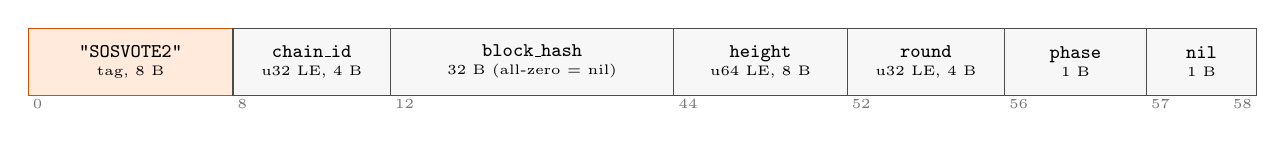
\begin{tikzpicture}
  \node[bft, minimum width=26mm] (v0) at (0,0) {\code{"SOSVOTE2"}\\[-1.5pt]\tiny tag, 8 B};
  \node[bf, minimum width=20mm, right=0mm of v0] (v1) {\code{chain\_id}\\[-1.5pt]\tiny u32 LE, 4 B};
  \node[bf, minimum width=36mm, right=0mm of v1] (v2) {\code{block\_hash}\\[-1.5pt]\tiny 32 B (all-zero $=$ nil)};
  \node[bf, minimum width=22mm, right=0mm of v2] (v3) {\code{height}\\[-1.5pt]\tiny u64 LE, 8 B};
  \node[bf, minimum width=20mm, right=0mm of v3] (v4) {\code{round}\\[-1.5pt]\tiny u32 LE, 4 B};
  \node[bf, minimum width=18mm, right=0mm of v4] (v5) {\code{phase}\\[-1.5pt]\tiny 1 B};
  \node[bf, minimum width=14mm, right=0mm of v5] (v6) {\code{nil}\\[-1.5pt]\tiny 1 B};
  \node[bfoff]  at (v0.south west) {0};
  \node[bfoff]  at (v1.south west) {8};
  \node[bfoff]  at (v2.south west) {12};
  \node[bfoff]  at (v3.south west) {44};
  \node[bfoff]  at (v4.south west) {52};
  \node[bfoff]  at (v5.south west) {56};
  \node[bfoff]  at (v6.south west) {57};
  \node[bfoffr] at (v6.south east) {58};
\end{tikzpicture}}%
\caption{The 58-byte vote-sign preimage (Construction~\ref{con:vote}),
signed raw with \mldsa{} (empty context). \code{phase} $= 0$
(\textsc{prevote}) or $1$ (\textsc{precommit}); \code{nil} $= 1$ iff
\code{block\_hash} is all-zero. The identical bytes are built by the node,
the light client, and the zkVM consensus and epoch guests.}
\label{fig:wire-vote}
\end{figure}

\subsection*{A.2 \quad Block-hash v4 preimage (after the domain tag)}
\begin{center}
\begin{tabular}{@{}llll@{}}
\toprule
\textbf{offset} & \textbf{len} & \textbf{field} & \textbf{encoding} \\
\midrule
0   & 4  & chain\_id            & u32 LE (current network \code{0x534F53}) \\
4   & 4  & epoch                & u32 LE \\
8   & 32 & validator\_set\_hash & Construction~\ref{con:valsethash} \\
40  & 8  & height               & u64 LE \\
48  & 8  & slot                 & u64 LE \\
56  & 32 & tx\_root             & \\
88  & 32 & utxo\_root           & \\
120 & 32 & ext\_root            & \\
152 & 32 & prev\_app\_hash      & \\
\bottomrule
\end{tabular}
\end{center}
Digest $= \sha{}(\code{"bqp:block:v4"} \concat \mathrm{preimage})$.

\begin{figure}[ht]\centering
% Layout source: crates/btp-proofs-shared/src/lib.rs:368-394 (block_hash_v4),
% byte-identical to the chain's compute_block_hash_v4 in consensus_reactor.rs.
\adjustbox{max width=\textwidth}{%
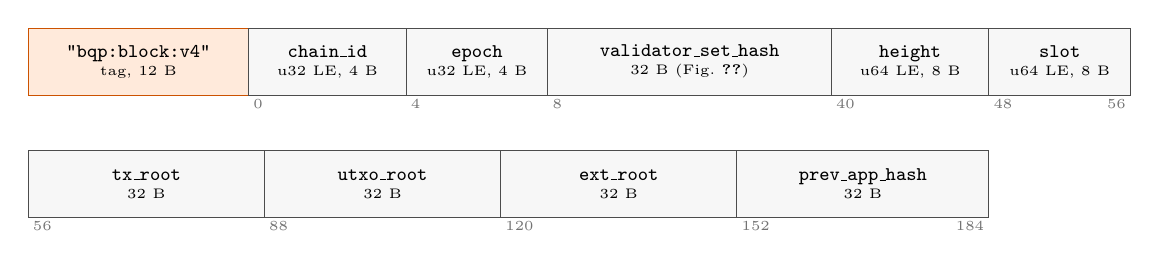
\begin{tikzpicture}
  % row 1
  \node[bft, minimum width=28mm] (b0) at (0,0) {\code{"bqp:block:v4"}\\[-1.5pt]\tiny tag, 12 B};
  \node[bf, minimum width=20mm, right=0mm of b0] (b1) {\code{chain\_id}\\[-1.5pt]\tiny u32 LE, 4 B};
  \node[bf, minimum width=18mm, right=0mm of b1] (b2) {\code{epoch}\\[-1.5pt]\tiny u32 LE, 4 B};
  \node[bf, minimum width=36mm, right=0mm of b2] (b3) {\code{validator\_set\_hash}\\[-1.5pt]\tiny 32 B (Fig.~\ref{fig:wire-valset})};
  \node[bf, minimum width=20mm, right=0mm of b3] (b4) {\code{height}\\[-1.5pt]\tiny u64 LE, 8 B};
  \node[bf, minimum width=18mm, right=0mm of b4] (b5) {\code{slot}\\[-1.5pt]\tiny u64 LE, 8 B};
  \node[bfoff]  at (b1.south west) {0};
  \node[bfoff]  at (b2.south west) {4};
  \node[bfoff]  at (b3.south west) {8};
  \node[bfoff]  at (b4.south west) {40};
  \node[bfoff]  at (b5.south west) {48};
  \node[bfoffr] at (b5.south east) {56};
  % row 2 (continuation)
  \node[bf, minimum width=30mm] (c0) at (0,-1.55) {\code{tx\_root}\\[-1.5pt]\tiny 32 B};
  \node[bf, minimum width=30mm, right=0mm of c0] (c1) {\code{utxo\_root}\\[-1.5pt]\tiny 32 B};
  \node[bf, minimum width=30mm, right=0mm of c1] (c2) {\code{ext\_root}\\[-1.5pt]\tiny 32 B};
  \node[bf, minimum width=32mm, right=0mm of c2] (c3) {\code{prev\_app\_hash}\\[-1.5pt]\tiny 32 B};
  \node[bfoff]  at (c0.south west) {56};
  \node[bfoff]  at (c1.south west) {88};
  \node[bfoff]  at (c2.south west) {120};
  \node[bfoff]  at (c3.south west) {152};
  \node[bfoffr] at (c3.south east) {184};
\end{tikzpicture}}%
\caption{The \code{bqp:block:v4} block-hash preimage
(Construction~\ref{con:blockhash}); digest $= \sha{}$ over the tag followed
by the 184 fixed-width payload bytes (offsets count the payload; the second
row continues the first). Because the quorum certificate signs this hash,
the four leading fields make the quorum attest the chain identity, the
epoch, and the canonical validator set --- the binding the bridge and PCF
rely on. Widths not to scale.}
\label{fig:wire-blockhash}
\end{figure}

\subsection*{A.3 \quad Validator-set hash preimage}
$\code{"sos:bridge-valset:v2"}$ then, per active validator in canonical
order (effective stake desc, id asc): \code{consensus\_pk} (1952) $\concat$
stake (u64 LE).

\begin{figure}[ht]\centering
% Layout source: crates/btp-proofs-shared/src/lib.rs:420-431
% (bridge_validator_set_hash); canonical active-pool order is supplied by the
% chain (effective stake desc, id asc) and is order-sensitive by construction.
\adjustbox{max width=\textwidth}{%
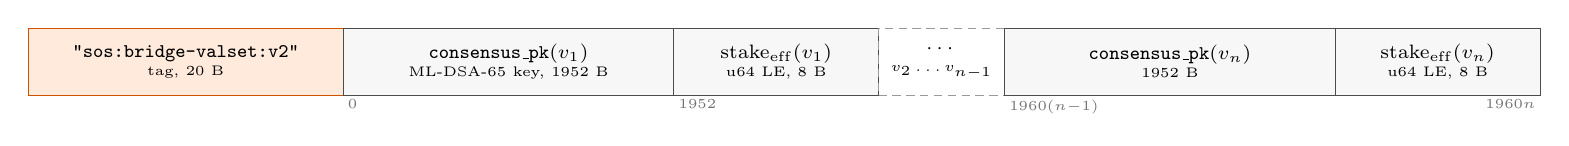
\begin{tikzpicture}
  \node[bft, minimum width=40mm] (s0) at (0,0) {\code{"sos:bridge-valset:v2"}\\[-1.5pt]\tiny tag, 20 B};
  \node[bf, minimum width=42mm, right=0mm of s0] (s1) {\code{consensus\_pk}$(v_1)$\\[-1.5pt]\tiny \mldsa{} key, 1952 B};
  \node[bf, minimum width=26mm, right=0mm of s1] (s2) {$\mathrm{stake}_{\mathrm{eff}}(v_1)$\\[-1.5pt]\tiny u64 LE, 8 B};
  \node[bfe, minimum width=16mm, right=0mm of s2] (s3) {$\cdots$\\[-1.5pt]\tiny $v_2 \ldots v_{n-1}$};
  \node[bf, minimum width=42mm, right=0mm of s3] (s4) {\code{consensus\_pk}$(v_n)$\\[-1.5pt]\tiny 1952 B};
  \node[bf, minimum width=26mm, right=0mm of s4] (s5) {$\mathrm{stake}_{\mathrm{eff}}(v_n)$\\[-1.5pt]\tiny u64 LE, 8 B};
  \node[bfoff]  at (s1.south west) {0};
  \node[bfoff]  at (s2.south west) {1952};
  \node[bfoff]  at (s4.south west) {$1960(n{-}1)$};
  \node[bfoffr] at (s5.south east) {$1960n$};
\end{tikzpicture}}%
\caption{The validator-set hash input (Construction~\ref{con:valsethash}):
$\sha{}$ over the tag, then one $(\code{consensus\_pk} \concat
\LE{8}(\mathrm{stake}_{\mathrm{eff}}))$ pair of 1960 bytes per active
validator in canonical active-pool order. The digest is bound inside the v4
block hash (Figure~\ref{fig:wire-blockhash}), recomputed by the consensus
guest from the supplied set, and tracked by the Ethereum contract. Widths
not to scale.}
\label{fig:wire-valset}
\end{figure}

\subsection*{A.4 \quad Bridge batch journal (Solidity \code{abi.encode})}
Head: \code{blockHash} (bytes32) $\concat$ \code{height} (uint64, 32-byte
BE word) $\concat$ \code{validatorSetHash} (bytes32) $\concat$ \code{epoch}
(uint32 word) $\concat$ \code{chainId} (uint32 word) $\concat$ offset
$= 192$ (word). Tail: array length (word), then per operation 128 bytes:
\code{lockId} (bytes32), \code{ethRecipient} (20 bytes right-aligned in a
word), \code{amount} (uint64 word), \code{relayFee} (uint64 word). The
contract verifies the seal against
$\mathrm{sha256}(\mathrm{these\ bytes})$.

\begin{figure}[ht]\centering
% Layout source: crates/btp-proofs-shared/src/lib.rs:519-553
% (bridge_batch_abi_journal, committed raw by the batch guest via
% env::commit_slice, btp-proofs-guest-bridge-batch/src/main.rs:69-81) and
% contracts/src/SOSBridge.sol:154-168 (processDeposits re-encodes the same
% fields from calldata and derives sha256(journal) on-chain).
\adjustbox{max width=\textwidth}{%
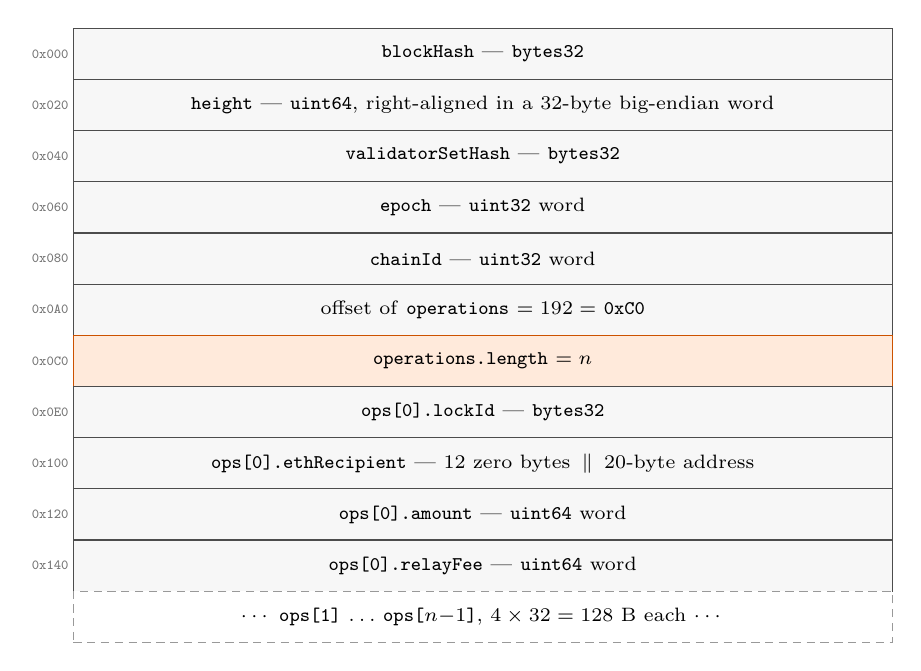
\begin{tikzpicture}
  \node[bfw]  (w0) at (0,0)            {\code{blockHash} --- \code{bytes32}};
  \node[bfw]  (w1) at (w0.south west)  {\code{height} --- \code{uint64}, right-aligned in a 32-byte big-endian word};
  \node[bfw]  (w2) at (w1.south west)  {\code{validatorSetHash} --- \code{bytes32}};
  \node[bfw]  (w3) at (w2.south west)  {\code{epoch} --- \code{uint32} word};
  \node[bfw]  (w4) at (w3.south west)  {\code{chainId} --- \code{uint32} word};
  \node[bfw]  (w5) at (w4.south west)  {offset of \code{operations} $= 192 =$ \code{0xC0}};
  \node[bfwt] (w6) at (w5.south west)  {\code{operations.length} $= n$};
  \node[bfw]  (w7) at (w6.south west)  {\code{ops[0].lockId} --- \code{bytes32}};
  \node[bfw]  (w8) at (w7.south west)  {\code{ops[0].ethRecipient} --- 12 zero bytes $\concat$ 20-byte address};
  \node[bfw]  (w9) at (w8.south west)  {\code{ops[0].amount} --- \code{uint64} word};
  \node[bfw]  (w10) at (w9.south west) {\code{ops[0].relayFee} --- \code{uint64} word};
  \node[bfwe] (w11) at (w10.south west){$\cdots$ \code{ops[1]} $\ldots$ \code{ops[}$n{-}1$\code{]}, $4 \times 32 = 128$ B each $\cdots$};
  \node[bfaddr] at (w0.west)  {0x000};
  \node[bfaddr] at (w1.west)  {0x020};
  \node[bfaddr] at (w2.west)  {0x040};
  \node[bfaddr] at (w3.west)  {0x060};
  \node[bfaddr] at (w4.west)  {0x080};
  \node[bfaddr] at (w5.west)  {0x0A0};
  \node[bfaddr] at (w6.west)  {0x0C0};
  \node[bfaddr] at (w7.west)  {0x0E0};
  \node[bfaddr] at (w8.west)  {0x100};
  \node[bfaddr] at (w9.west)  {0x120};
  \node[bfaddr] at (w10.west) {0x140};
\end{tikzpicture}}%
\caption{The bridge-batch ABI journal (Section~\ref{sec:journal}): the exact
$\mathrm{abi.encode}(\code{blockHash}, \code{height},
\code{validatorSetHash}, \code{epoch}, \code{chainId}, \code{operations[]})$
bytes the batch guest commits raw (\code{env::commit\_slice}) and the
\code{SOSBridge} contract re-encodes from its own calldata; six 32-byte head
words (the sixth is the offset of the dynamic array), the array length, then
one 128-byte static tuple per operation. The seal is verified against
$\mathrm{sha256}$ of exactly these bytes, derived on-chain --- never
supplied.}
\label{fig:wire-journal}
\end{figure}

\subsection*{A.5 \quad Note plaintext (83 bytes)}
value (u64 LE, 8) $\concat$ $d$ (11) $\concat$ $\rho$ (32) $\concat$
$\mathit{rcm}$ (32); sealed per Construction~\ref{con:sealed} with
$\mathrm{AAD} = \mathit{cm}$.

\begin{figure}[ht]\centering
% Layout source: crates/btp-note-core/src/lib.rs:50 (NOTE_PLAINTEXT_LEN = 83)
% and lib.rs:271-298 (note_plaintext_encode / note_plaintext_decode).
\adjustbox{max width=\textwidth}{%
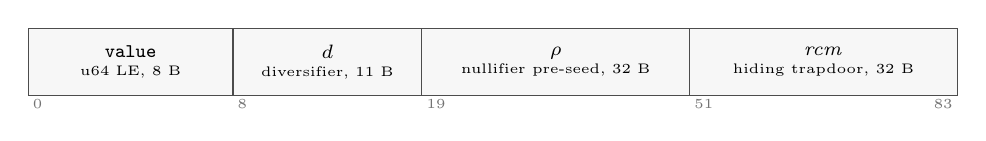
\begin{tikzpicture}
  \node[bf, minimum width=26mm] (p0) at (0,0) {\code{value}\\[-1.5pt]\tiny u64 LE, 8 B};
  \node[bf, minimum width=24mm, right=0mm of p0] (p1) {$d$\\[-1.5pt]\tiny diversifier, 11 B};
  \node[bf, minimum width=34mm, right=0mm of p1] (p2) {$\rho$\\[-1.5pt]\tiny nullifier pre-seed, 32 B};
  \node[bf, minimum width=34mm, right=0mm of p2] (p3) {$\mathit{rcm}$\\[-1.5pt]\tiny hiding trapdoor, 32 B};
  \node[bfoff]  at (p0.south west) {0};
  \node[bfoff]  at (p1.south west) {8};
  \node[bfoff]  at (p2.south west) {19};
  \node[bfoff]  at (p3.south west) {51};
  \node[bfoffr] at (p3.south east) {83};
\end{tikzpicture}}%
\caption{The 83-byte note plaintext (Construction~\ref{con:sealed}) --- the
minimal data a recipient needs to recognize and later spend a note; the
recipient already holds $\mathit{ak}/\mathit{nk}$ and re-derives
$\mathit{npk}$, then recomputes \code{commit\_v3} and accepts only on
equality with the on-chain commitment.}
\label{fig:wire-noteplain}
\end{figure}

\subsection*{A.6 \quad Note commitment and nullifier preimages}
\code{commit\_v3} input: tag $\concat$ value (u64 LE) $\concat$
$\mathit{ak}$ $\concat$ $\mathit{npk}$ $\concat$ $d$ $\concat$ $\rho$
$\concat$ $\mathit{rcm}$ (147 payload bytes); nullifier input: tag
$\concat$ $\mathit{nk}$ $\concat$ $\rho$ $\concat$ position (u64 LE)
(72 payload bytes). Both are \shake{} squeezed to 32 bytes.

\begin{figure}[ht]\centering
% Layout sources: crates/btp-note-core/src/lib.rs:202-211 (commit_v3:
% SHAKE256("sos:note-commit:v3" || LE64(value) || ak || npk || d || rho || rcm))
% and lib.rs:235-237 (nullifier: SHAKE256("sos:nullifier:v2" || nk || rho ||
% LE64(position))).
\adjustbox{max width=\textwidth}{%
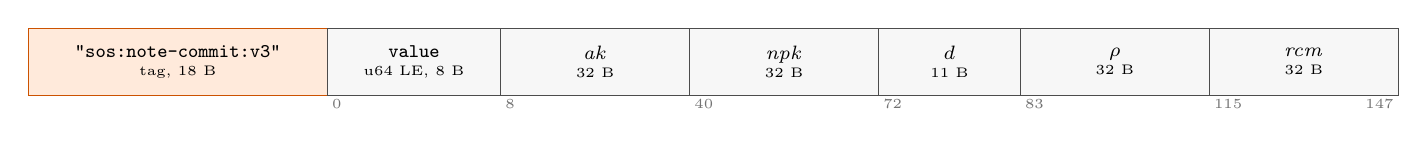
\begin{tikzpicture}
  \node[bft, minimum width=38mm] (m0) at (0,0) {\code{"sos:note-commit:v3"}\\[-1.5pt]\tiny tag, 18 B};
  \node[bf, minimum width=22mm, right=0mm of m0] (m1) {\code{value}\\[-1.5pt]\tiny u64 LE, 8 B};
  \node[bf, minimum width=24mm, right=0mm of m1] (m2) {$\mathit{ak}$\\[-1.5pt]\tiny 32 B};
  \node[bf, minimum width=24mm, right=0mm of m2] (m3) {$\mathit{npk}$\\[-1.5pt]\tiny 32 B};
  \node[bf, minimum width=18mm, right=0mm of m3] (m4) {$d$\\[-1.5pt]\tiny 11 B};
  \node[bf, minimum width=24mm, right=0mm of m4] (m5) {$\rho$\\[-1.5pt]\tiny 32 B};
  \node[bf, minimum width=24mm, right=0mm of m5] (m6) {$\mathit{rcm}$\\[-1.5pt]\tiny 32 B};
  \node[bfoff]  at (m1.south west) {0};
  \node[bfoff]  at (m2.south west) {8};
  \node[bfoff]  at (m3.south west) {40};
  \node[bfoff]  at (m4.south west) {72};
  \node[bfoff]  at (m5.south west) {83};
  \node[bfoff]  at (m6.south west) {115};
  \node[bfoffr] at (m6.south east) {147};
\end{tikzpicture}}\\[3mm]
\adjustbox{max width=\textwidth}{%
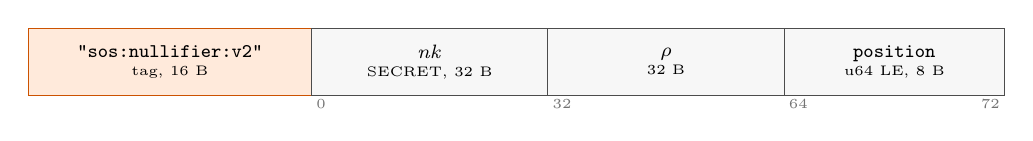
\begin{tikzpicture}
  \node[bft, minimum width=36mm] (n0) at (0,0) {\code{"sos:nullifier:v2"}\\[-1.5pt]\tiny tag, 16 B};
  \node[bf, minimum width=30mm, right=0mm of n0] (n1) {$\mathit{nk}$\\[-1.5pt]\tiny SECRET, 32 B};
  \node[bf, minimum width=30mm, right=0mm of n1] (n2) {$\rho$\\[-1.5pt]\tiny 32 B};
  \node[bf, minimum width=28mm, right=0mm of n2] (n3) {\code{position}\\[-1.5pt]\tiny u64 LE, 8 B};
  \node[bfoff]  at (n1.south west) {0};
  \node[bfoff]  at (n2.south west) {32};
  \node[bfoff]  at (n3.south west) {64};
  \node[bfoffr] at (n3.south east) {72};
\end{tikzpicture}}%
\caption{The ownership-welded note commitment \code{commit\_v3} (top) and
the position-bound nullifier (bottom), both
$\mathrm{SHAKE256}_{32}(\mathrm{tag} \concat \cdots)$
(Construction~\ref{con:note}). The weld: $\mathit{npk} =
S_{\code{sos:npk:v1}}(\mathit{nk} \concat \mathit{ak})$ is committed in
$\mathit{cm}$ while the spend circuit witnesses $\mathit{nk}$ and feeds the
\emph{same} $\mathit{nk}$ into the nullifier (Section~\ref{sec:ownership});
the leaf position makes nullifiers distinct even across colliding $\rho$.}
\label{fig:wire-note-binds}
\end{figure}

\subsection*{A.7 \quad Sealed-note blob and AEAD key derivation}
On-chain blob: \code{kem\_ct} (1568) $\concat$ \code{aead\_ct}
(plaintext length $+$ 16-byte Poly1305 tag), stored with a separate 1-byte
view tag; $\mathrm{AAD} = \mathit{cm}$. Key material: $\mathrm{SHAKE256}_{45}
(\code{"sos:note-aead:v1"} \concat \mathit{ss})$ split as key (32)
$\concat$ nonce (12) $\concat$ view tag (1).

\begin{figure}[ht]\centering
% Layout source: crates/sos-crypto/src/note_aead.rs:11-19 (format comment),
% :37-45 (KEM_CT_LEN = 1568, AEAD_TAG_LEN = 16, 45-byte keymat), :60-82
% (to_blob/from_blob: blob = kem_ct || ciphertext; view_tag stored alongside),
% :96-105 (seal: AAD = cm). Plaintext length 83 per Figure A.5.
\adjustbox{max width=\textwidth}{%
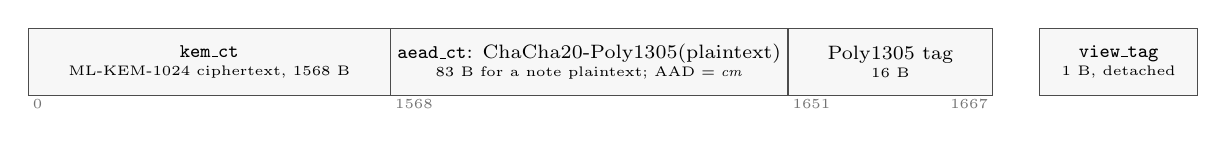
\begin{tikzpicture}
  \node[bf, minimum width=46mm] (e0) at (0,0) {\code{kem\_ct}\\[-1.5pt]\tiny \mlkem{} ciphertext, 1568 B};
  \node[bf, minimum width=44mm, right=0mm of e0] (e1) {\code{aead\_ct}: ChaCha20-Poly1305(plaintext)\\[-1.5pt]\tiny 83 B for a note plaintext; $\mathrm{AAD} = \mathit{cm}$};
  \node[bf, minimum width=26mm, right=0mm of e1] (e2) {Poly1305 tag\\[-1.5pt]\tiny 16 B};
  \node[bf, minimum width=20mm, right=6mm of e2] (e3) {\code{view\_tag}\\[-1.5pt]\tiny 1 B, detached};
  \node[bfoff]  at (e0.south west) {0};
  \node[bfoff]  at (e1.south west) {1568};
  \node[bfoff]  at (e2.south west) {1651};
  \node[bfoffr] at (e2.south east) {1667};
\end{tikzpicture}}\\[3mm]
\adjustbox{max width=\textwidth}{%
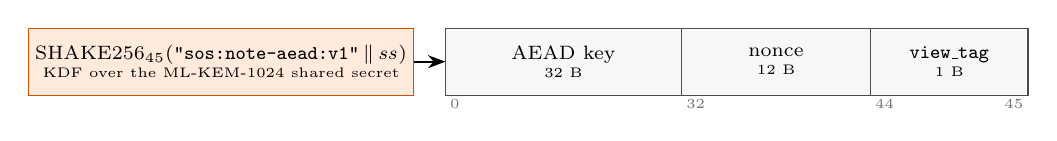
\begin{tikzpicture}
  \node[bft, minimum width=46mm] (k0) at (0,0) {$\mathrm{SHAKE256}_{45}(\code{"sos:note-aead:v1"} \concat \mathit{ss})$\\[-1.5pt]\tiny KDF over the \mlkem{} shared secret};
  \node[bf, minimum width=30mm, right=4mm of k0] (k1) {AEAD key\\[-1.5pt]\tiny 32 B};
  \node[bf, minimum width=24mm, right=0mm of k1] (k2) {nonce\\[-1.5pt]\tiny 12 B};
  \node[bf, minimum width=20mm, right=0mm of k2] (k3) {\code{view\_tag}\\[-1.5pt]\tiny 1 B};
  \draw[arr] (k0.east) -- (k1.west);
  \node[bfoff]  at (k1.south west) {0};
  \node[bfoff]  at (k2.south west) {32};
  \node[bfoff]  at (k3.south west) {44};
  \node[bfoffr] at (k3.south east) {45};
\end{tikzpicture}}%
\caption{Top: the on-chain sealed-note blob (Construction~\ref{con:sealed})
--- a fresh \mlkem{} ciphertext followed by the AEAD ciphertext and tag
(1667 bytes for the 83-byte note plaintext), with the one-byte view tag
stored as a separate field. Bottom: the 45-byte key-material split derived
by \shake{} from the encapsulated shared secret $\mathit{ss}$; the derived
nonce is single-use by construction because $\mathit{ss}$ is fresh per
note. Binding $\mathrm{AAD} = \mathit{cm}$ welds the blob to exactly one
commitment. Widths not to scale.}
\label{fig:wire-sealed}
\end{figure}

\subsection*{A.8 \quad Guest journal layouts (consensus and PCF epoch guests)}
The consensus guest and the PCF epoch-checkpoint guest commit \emph{typed}
journals: the field sequences below, serialized by the zkVM's canonical
little-endian 32-bit-word serializer (\code{env::commit}) and decoded by
their (pinned) consumers with the same library --- so the wire encoding is
library-defined and host/guest-identical by construction, and the
security-relevant binding is at the typed-field level. The bridge-batch
journal is the exception: it is hand-specified raw bytes (A.4,
Figure~\ref{fig:wire-journal}), because an Ethereum contract must re-derive
it.

\begin{figure}[ht]\centering
% Field sources: crates/btp-proofs-shared/src/lib.rs:231-244
% (ConsensusProofOutput; committed by btp-proofs-guest-consensus/src/main.rs:
% 104-116 via env::commit and decoded by the batch guest with
% risc0_zkvm::serde::from_slice) and lib.rs:288-308 (EpochCheckpointOutput,
% the PCF certificate journal; blocks_commitment = epoch_blocks_commitment,
% lib.rs:315-332).
{\footnotesize (a) consensus guest --- \code{ConsensusProofOutput}}\\[1mm]
\adjustbox{max width=\textwidth}{%
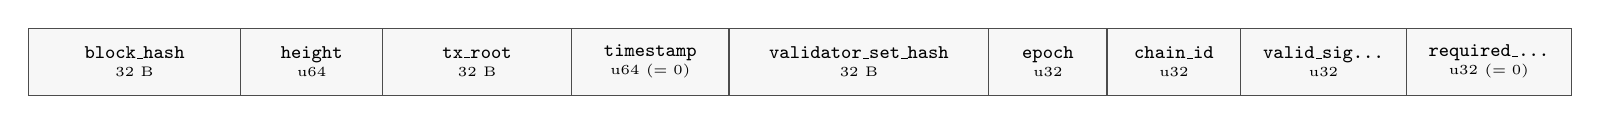
\begin{tikzpicture}
  \node[bf, minimum width=27mm] (j0) at (0,0) {\code{block\_hash}\\[-1.5pt]\tiny 32 B};
  \node[bf, minimum width=18mm, right=0mm of j0] (j1) {\code{height}\\[-1.5pt]\tiny u64};
  \node[bf, minimum width=24mm, right=0mm of j1] (j2) {\code{tx\_root}\\[-1.5pt]\tiny 32 B};
  \node[bf, minimum width=20mm, right=0mm of j2] (j3) {\code{timestamp}\\[-1.5pt]\tiny u64 ($=0$)};
  \node[bf, minimum width=33mm, right=0mm of j3] (j4) {\code{validator\_set\_hash}\\[-1.5pt]\tiny 32 B};
  \node[bf, minimum width=15mm, right=0mm of j4] (j5) {\code{epoch}\\[-1.5pt]\tiny u32};
  \node[bf, minimum width=17mm, right=0mm of j5] (j6) {\code{chain\_id}\\[-1.5pt]\tiny u32};
  \node[bf, minimum width=21mm, right=0mm of j6] (j7) {\code{valid\_sig...}\\[-1.5pt]\tiny u32};
  \node[bf, minimum width=21mm, right=0mm of j7] (j8) {\code{required\_...}\\[-1.5pt]\tiny u32 ($=0$)};
\end{tikzpicture}}\\[3mm]
{\footnotesize (b) PCF epoch-checkpoint guest --- \code{EpochCheckpointOutput}
(Construction~\ref{con:pcf})}\\[1mm]
\adjustbox{max width=\textwidth}{%
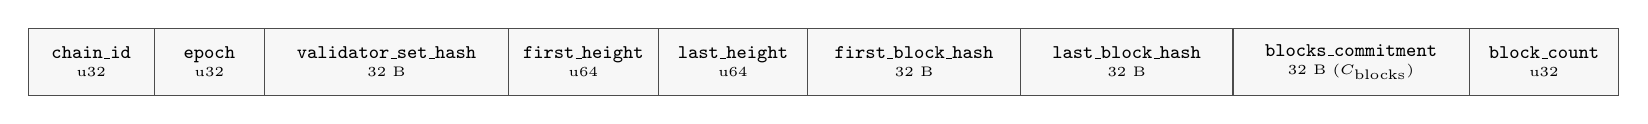
\begin{tikzpicture}
  \node[bf, minimum width=16mm] (q0) at (0,0) {\code{chain\_id}\\[-1.5pt]\tiny u32};
  \node[bf, minimum width=14mm, right=0mm of q0] (q1) {\code{epoch}\\[-1.5pt]\tiny u32};
  \node[bf, minimum width=31mm, right=0mm of q1] (q2) {\code{validator\_set\_hash}\\[-1.5pt]\tiny 32 B};
  \node[bf, minimum width=19mm, right=0mm of q2] (q3) {\code{first\_height}\\[-1.5pt]\tiny u64};
  \node[bf, minimum width=19mm, right=0mm of q3] (q4) {\code{last\_height}\\[-1.5pt]\tiny u64};
  \node[bf, minimum width=27mm, right=0mm of q4] (q5) {\code{first\_block\_hash}\\[-1.5pt]\tiny 32 B};
  \node[bf, minimum width=27mm, right=0mm of q5] (q6) {\code{last\_block\_hash}\\[-1.5pt]\tiny 32 B};
  \node[bf, minimum width=30mm, right=0mm of q6] (q7) {\code{blocks\_commitment}\\[-1.5pt]\tiny 32 B ($C_{\mathrm{blocks}}$)};
  \node[bf, minimum width=19mm, right=0mm of q7] (q8) {\code{block\_count}\\[-1.5pt]\tiny u32};
\end{tikzpicture}}%
\caption{Typed journal field sequences of the consensus guest (top;
Section~\ref{sec:consensus-guest}) and the PCF epoch-checkpoint guest
(bottom; Construction~\ref{con:pcf}). \code{timestamp} and
\code{required\_signatures} are committed as fixed zeros by the current
guest; $C_{\mathrm{blocks}}$ is the \code{sos:epoch-blocks:v1/:step} hash
chain that lets one epoch receipt authenticate any interior block and its
\code{tx\_root}. Field widths are the logical (in-struct) widths, not wire
bytes: both journals are encoded by the zkVM's word-oriented serializer,
identically on host and guest.}
\label{fig:wire-guest-journals}
\end{figure}

\section{Domain-Separation Tag Registry}
\label{app:domains}

\begin{center}
\adjustbox{max width=\textwidth}{%
\small
\begin{tabular}{@{}lll@{}}
\toprule
\textbf{tag} & \textbf{hash} & \textbf{purpose} \\
\midrule
\code{bqp:block:v2/v3/v4}        & \sha{}   & block hash preimages (version-gated) \\
\code{bqp:validator-pk:v1}       & \sha{}   & validator identity from consensus key \\
\code{sos:weighted-proposer:v2}  & \sha{}   & weighted proposer-permutation draws \\
\code{sos:bridge-valset:v2}      & \sha{}   & canonical validator-set hash \\
\code{bqp:txid:v1}               & \sha{}   & transaction id \\
\code{bqp:merkle:v1}             & \sha{}   & tx-tree node (sorted-pair) \\
\code{bqp:private-pool:v4}       & \sha{}   & shielded-pool component of \code{app\_hash} \\
\code{sos:epoch-blocks:v1/:step} & \sha{}   & PCF per-epoch block commitment chain \\
\code{sos:note-rcm:v1}, \code{sos:note-rho:v1}, \code{sos:note-psi:v1} & \shake{} & per-note randomness derivation \\
\code{sos:ak:v1}, \code{sos:nk:v1}, \code{sos:npk:v1} & \shake{} & key derivations (Construction~\ref{con:keys}) \\
\code{sos:note-commit:v2/v3}     & \shake{} & note commitment (v3 = ownership-welded) \\
\code{sos:nullifier:v2}          & \shake{} & nullifier \\
\code{sos:addr-pkd:v1}           & \shake{} & diversified transmission key \\
\code{sos:cmt-node:v1}, \code{sos:cmt-empty:v1} & \shake{} & commitment-tree nodes / empty leaf \\
\code{sos:unshield-recipient:v1} & \shake{} & unshield destination binding \\
\code{sos:note-aead:v1}          & \shake{} & note AEAD KDF (45-byte output) \\
\code{bqp:shield-auth:v1}        & \sha{}   & shield authorization signature domain \\
\code{bqp:burn:v1}               & \sha{}   & Ethereum-side wSOS-burn replay id (reverse bridge) \\
\code{sos:airdrop-leaf:v1}, \code{sos:airdrop-node:v1}, \code{sos:airdrop-claim:v1} & \sha{} & Merkle-drop commitment and claim \\
\bottomrule
\end{tabular}}
\end{center}

Rules: a tag is never reused across purposes; semantic changes bump the
version suffix behind an activation gate; both the \code{bqp:} and
\code{sos:} namespaces are frozen constants.

\section{Parameter Summary}
\label{app:params}

\begin{center}
\adjustbox{max width=\textwidth}{%
\small
\begin{tabular}{@{}lll@{}}
\toprule
\textbf{parameter} & \textbf{value} & \textbf{where} \\
\midrule
signature scheme              & \mldsa{} (FIPS 204, cat.\ 3; pk 1952 B, sig 3309 B) & \S\ref{sec:mldsa} \\
note encryption               & \mlkem{} (FIPS 203, cat.\ 5) + ChaCha20-Poly1305 & \S\ref{sec:notes-enc} \\
hashes                        & \sha{} / \shake{} (32-byte outputs) & \S\ref{sec:sha3} \\
chain id                      & \code{0x534F53} & \S\ref{sec:blockhash} \\
supply cap                    & 21{,}000{,}000 SOS ($2.1\times10^{15}$ sats) & \S\ref{sec:economics} \\
genesis supply / emission pool & 2{,}100{,}000 SOS (10\%) / 18{,}900{,}000 SOS (90\%) & \S\ref{sec:claim} \\
emission                      & 210{,}000 SOS/yr; 7-day epochs; 70/20/10 split; 30\% fee burn; cap-truncated & \S\ref{sec:emission} \\
unbonding period              & 21 days & \S\ref{sec:staking} \\
slashing                      & double-sign 5\%; downtime jail; other burns reserved & \S\ref{sec:slashing} \\
consensus tick / commit       & 200 ms tick; $\approx$600 ms (4-node), $\approx$0.63 s (live 1-val) & \S\ref{sec:consensus-eval} \\
max block size                & 4 MiB (incl.\ consensus envelope) & \S\ref{sec:liveness} \\
validator pool / signers      & 200 pool / 64 active signers per block (genesis) & \S\ref{sec:valset} \\
launch active set             & $N \le 128$ & \S\ref{sec:bounded} \\
quorum rule                   & strict $>2/3$ effective stake; distinct signers & \S\ref{sec:qc} \\
round-sync rule               & strict $>1/3$ effective stake at a higher round & \S\ref{sec:liveness} \\
commitment tree               & depth 32, \shake{} nodes & \S\ref{sec:notes} \\
anchor window                 & 256 distinct recent roots, in \code{app\_hash} & \S\ref{sec:circuits} \\
value bound (shielded)        & $< 2^{51}$ sats per note/fee & \S\ref{sec:circuits} \\
note plaintext / view tag     & 83 B / 1 B & \S\ref{sec:notes-enc} \\
in-zkVM \mldsa{} verify       & $\approx$5.87 M cycles ($\approx$3.67 M with S1) & \S\ref{sec:accel} \\
AIR in-guest verify (M1pp)    & $\approx$174 M cycles; $K^\ast \approx 47$ (baked VK) & \S\ref{sec:airtrack} \\
\bottomrule
\end{tabular}}
\end{center}

% ============================================================================
% Inline, self-contained bibliography (no BibTeX / sos-v2.bib required):
% a single pdfLaTeX pass resolves every \cite. (sos-v2.bib is retained in the
% repo as the BibTeX source of record but is not needed to compile.)
\begin{thebibliography}{99}
\addcontentsline{toc}{section}{References}

\bibitem{nakamoto2008} S.~Nakamoto. \emph{Bitcoin: A Peer-to-Peer Electronic Cash System}. 2008. \url{https://bitcoin.org/bitcoin.pdf}
\bibitem{wood2014} G.~Wood. \emph{Ethereum: A Secure Decentralised Generalised Transaction Ledger}. Ethereum Yellow Paper, 2014. \url{https://ethereum.github.io/yellowpaper/paper.pdf}
\bibitem{shor1997} P.~W.~Shor. \emph{Polynomial-Time Algorithms for Prime Factorization and Discrete Logarithms on a Quantum Computer}. SIAM J. Comput.\ 26(5):1484--1509, 1997.
\bibitem{grover1996} L.~K.~Grover. \emph{A Fast Quantum Mechanical Algorithm for Database Search}. STOC 1996, 212--219.
\bibitem{mosca2018} M.~Mosca. \emph{Cybersecurity in an Era with Quantum Computers: Will We Be Ready?} IEEE Security \& Privacy 16(5):38--41, 2018.
\bibitem{nistir8413} G.~Alagic et al. \emph{Status Report on the Third Round of the NIST Post-Quantum Cryptography Standardization Process}. NIST IR 8413, 2022. \url{https://doi.org/10.6028/NIST.IR.8413}
\bibitem{fips202} NIST. \emph{FIPS 202: SHA-3 Standard: Permutation-Based Hash and Extendable-Output Functions}. 2015. \url{https://doi.org/10.6028/NIST.FIPS.202}
\bibitem{fips203} NIST. \emph{FIPS 203: Module-Lattice-Based Key-Encapsulation Mechanism Standard (ML-KEM)}. 2024. \url{https://doi.org/10.6028/NIST.FIPS.203}
\bibitem{fips204} NIST. \emph{FIPS 204: Module-Lattice-Based Digital Signature Standard (ML-DSA)}. 2024. \url{https://doi.org/10.6028/NIST.FIPS.204}
\bibitem{fips205} NIST. \emph{FIPS 205: Stateless Hash-Based Digital Signature Standard (SLH-DSA)}. 2024. \url{https://doi.org/10.6028/NIST.FIPS.205}
\bibitem{dilithium2018} L.~Ducas, E.~Kiltz, T.~Lepoint, V.~Lyubashevsky, P.~Schwabe, G.~Seiler, D.~Stehl\'e. \emph{CRYSTALS-Dilithium: A Lattice-Based Digital Signature Scheme}. IACR TCHES 2018(1):238--268.
\bibitem{kyber2018} J.~Bos, L.~Ducas, E.~Kiltz, T.~Lepoint, V.~Lyubashevsky, J.~M.~Schanck, P.~Schwabe, G.~Seiler, D.~Stehl\'e. \emph{CRYSTALS-Kyber: A CCA-Secure Module-Lattice-Based KEM}. IEEE EuroS\&P 2018.
\bibitem{rfc8439} Y.~Nir, A.~Langley. \emph{ChaCha20 and Poly1305 for IETF Protocols}. RFC 8439, 2018. \url{https://www.rfc-editor.org/rfc/rfc8439}
\bibitem{rfc8391} A.~Huelsing, D.~Butin, S.-L.~Gazdag, J.~Rijneveld, A.~Mohaisen. \emph{XMSS: eXtended Merkle Signature Scheme}. RFC 8391, 2018.
\bibitem{starks2018} E.~Ben-Sasson, I.~Bentov, Y.~Horesh, M.~Riabzev. \emph{Scalable, Transparent, and Post-Quantum Secure Computational Integrity}. IACR ePrint 2018/046. \url{https://eprint.iacr.org/2018/046}
\bibitem{fri2018} E.~Ben-Sasson, I.~Bentov, Y.~Horesh, M.~Riabzev. \emph{Fast Reed-Solomon Interactive Oracle Proofs of Proximity}. ICALP 2018.
\bibitem{bcs2016} E.~Ben-Sasson, A.~Chiesa, N.~Spooner. \emph{Interactive Oracle Proofs}. TCC 2016.
\bibitem{ethstark2021} StarkWare. \emph{ethSTARK Documentation}. IACR ePrint 2021/582. \url{https://eprint.iacr.org/2021/582}
\bibitem{cms2019} A.~Chiesa, P.~Manohar, N.~Spooner. \emph{Succinct Arguments in the Quantum Random Oracle Model}. TCC 2019.
\bibitem{pcd2010} A.~Chiesa, E.~Tromer. \emph{Proof-Carrying Data and Hearsay Arguments from Signature Cards}. ICS 2010.
\bibitem{risc0} RISC Zero, Inc. \emph{RISC Zero: A General-Purpose Zero-Knowledge Virtual Machine (zkVM)}. 2023. \url{https://dev.risczero.com}
\bibitem{plonky3} Polygon Zero / Plonky3 contributors. \emph{Plonky3: A Toolkit for Polynomial IOPs and AIR-Based Proof Systems}. 2024. \url{https://github.com/Plonky3/Plonky3}
\bibitem{plonky3audit2024} Least Authority. \emph{Polygon Plonky3 Security Audit Report}. 2024.
\bibitem{groth16} J.~Groth. \emph{On the Size of Pairing-Based Non-interactive Arguments}. EUROCRYPT 2016.
\bibitem{pbft1999} M.~Castro, B.~Liskov. \emph{Practical Byzantine Fault Tolerance}. OSDI 1999.
\bibitem{dls1988} C.~Dwork, N.~Lynch, L.~Stockmeyer. \emph{Consensus in the Presence of Partial Synchrony}. JACM 35(2):288--323, 1988.
\bibitem{flp1985} M.~J.~Fischer, N.~A.~Lynch, M.~S.~Paterson. \emph{Impossibility of Distributed Consensus with One Faulty Process}. JACM 32(2):374--382, 1985.
\bibitem{tendermint2016} E.~Buchman. \emph{Tendermint: Byzantine Fault Tolerance in the Age of Blockchains}. M.Sc.\ thesis, University of Guelph, 2016. \url{https://hdl.handle.net/10214/9769}
\bibitem{tendermint2018} E.~Buchman, J.~Kwon, Z.~Milosevic. \emph{The Latest Gossip on BFT Consensus}. arXiv:1807.04938, 2018. \url{https://arxiv.org/abs/1807.04938}
\bibitem{hotstuff2019} M.~Yin, D.~Malkhi, M.~K.~Reiter, G.~Golan-Gueta, I.~Abraham. \emph{HotStuff: BFT Consensus with Linearity and Responsiveness}. ACM PODC 2019.
\bibitem{algorand2017} Y.~Gilad, R.~Hemo, S.~Micali, G.~Vlachos, N.~Zeldovich. \emph{Algorand: Scaling Byzantine Agreements for Cryptocurrencies}. ACM SOSP 2017.
\bibitem{compactcerts2020} S.~Micali, L.~Reyzin, G.~Vlachos, R.~S.~Wahby, N.~Zeldovich. \emph{Compact Certificates of Collective Knowledge}. IACR ePrint 2020/1568; IEEE S\&P 2021.
\bibitem{cometbft} CometBFT contributors. \emph{CometBFT: Proposer Selection and Validator Documentation}. 2024. \url{https://docs.cometbft.com}
\bibitem{mimblewimble2016} T.~E.~Jedusor. \emph{Mimblewimble}. 2016. \url{https://docs.beam.mw/Mimblewimble.pdf}
\bibitem{poelstra2016} A.~Poelstra. \emph{Mimblewimble}. 2016. \url{https://download.wpsoftware.net/bitcoin/wizardry/mimblewimble.pdf}
\bibitem{mweb2020} D.~Burkett. \emph{Mimblewimble Extension Blocks (MWEB), LIP-0002/0003}. Litecoin Improvement Proposals, 2020. \url{https://github.com/litecoin-project/lips}
\bibitem{zerocash2014} E.~Ben-Sasson, A.~Chiesa, C.~Garman, M.~Green, I.~Miers, E.~Tromer, M.~Virza. \emph{Zerocash: Decentralized Anonymous Payments from Bitcoin}. IEEE S\&P 2014.
\bibitem{zcashspec} D.~Hopwood, S.~Bowe, T.~Hornby, N.~Wilcox. \emph{Zcash Protocol Specification}. Version 2022.3.8, 2022. \url{https://zips.z.cash/protocol/protocol.pdf}
\bibitem{qrl2017} P.~Waterland. \emph{Quantum Resistant Ledger (QRL)}. Project whitepaper, November 2016. \url{https://github.com/theQRL/Whitepaper}
\bibitem{abelian2023} Abelian Project. \emph{Abelian (ABEL): A Quantum-Resistant Cryptocurrency Balancing Privacy and Accountability}. Whitepaper, 2022. \url{https://download.abelian.info/release/docs/whitepaper.pdf}
\bibitem{matrict2019} M.~F.~Esgin, R.~K.~Zhao, R.~Steinfeld, J.~K.~Liu, D.~Liu. \emph{MatRiCT: Efficient, Scalable and Post-Quantum Blockchain Confidential Transactions Protocol}. ACM CCS 2019, 567--584. \url{https://ia.cr/2019/1287}
\bibitem{matrictplus2022} M.~F.~Esgin, R.~Steinfeld, R.~K.~Zhao. \emph{MatRiCT$^{+}$: More Efficient Post-Quantum Private Blockchain Payments}. IEEE S\&P 2022, 1281--1298. \url{https://ia.cr/2021/545}
\bibitem{bls2003} D.~Boneh, B.~Lynn, H.~Shacham. \emph{Short Signatures from the Weil Pairing}. ASIACRYPT 2001; J. Cryptology 17(4), 2004.
\bibitem{altair2021} Ethereum Foundation. \emph{The Beacon Chain Altair Light Client Sync Protocol}. Ethereum consensus specifications, 2021. \url{https://github.com/ethereum/consensus-specs}
\bibitem{popos2022} S.~Agrawal, J.~Neu, E.~N.~Tas, D.~Zindros. \emph{Proofs of Proof-of-Stake with Sublinear Complexity}. arXiv:2209.08673, 2022.
\bibitem{succinct2022} Succinct Labs. \emph{Proof of Consensus: A ZK Light Client for Ethereum Proof-of-Stake}. 2022. \url{https://www.succinct.xyz}
\bibitem{weaksubj2014} V.~Buterin. \emph{Proof of Stake: How I Learned to Love Weak Subjectivity}. Ethereum Foundation blog, 2014.
\bibitem{squirrel2022} N.~Fleischhacker, M.~Simkin, Z.~Zhang. \emph{Squirrel: Efficient Synchronized Multi-Signatures from Lattices}. ACM CCS 2022.
\bibitem{chipmunk2023} N.~Fleischhacker, G.~Herold, M.~Simkin, Z.~Zhang. \emph{Chipmunk: Better Synchronized Multi-Signatures from Lattices}. ACM CCS 2023.
\bibitem{lemur2026} Lemur authors. \emph{Lemur: Scalable Post-Quantum Synchronized Multi-Signatures}. IACR ePrint 2026/1161.
\bibitem{lbvrf2021} Z.~Li et al. \emph{Post-Quantum VRF and its Applications in Future-Proof Blockchain}. arXiv:2109.02012, 2021.

\end{thebibliography}

\end{document}
